\documentclass[a4paper,12pt,twoside]{memoir}

% Castellano
\usepackage[spanish,es-tabla]{babel}
\selectlanguage{spanish}
\usepackage[utf8]{inputenc}
\usepackage[T1]{fontenc}
\usepackage{lmodern} % scalable font
\usepackage{microtype}
\usepackage{placeins}
\usepackage{pdflscape}


\RequirePackage{booktabs}
\RequirePackage[table]{xcolor}
\RequirePackage{xtab}
\RequirePackage{multirow}

\DeclareUnicodeCharacter{202F}{\,}


% Links
\PassOptionsToPackage{hyphens}{url}\usepackage[colorlinks]{hyperref}
\hypersetup{
	allcolors = {red}
}

% Ecuaciones
\usepackage{amsmath}

% Rutas de fichero / paquete
\newcommand{\ruta}[1]{{\sffamily #1}}

% Párrafos
\nonzeroparskip

% Huérfanas y viudas
\widowpenalty100000
\clubpenalty100000

% Evitar solapes en el header
\nouppercaseheads

% Imagenes
\usepackage{graphicx}
\newcommand{\imagen}[2]{
	\begin{figure}[!h]
		\centering
		\includegraphics[width=0.9\textwidth]{#1}
		\caption{#2}\label{fig:#1}
	\end{figure}
	\FloatBarrier
}

\newcommand{\imagenflotante}[2]{
	\begin{figure}%[!h]
		\centering
		\includegraphics[width=0.9\textwidth]{#1}
		\caption{#2}\label{fig:#1}
	\end{figure}
}



% El comando \figura nos permite insertar figuras comodamente, y utilizando
% siempre el mismo formato. Los parametros son:
% 1 -> Porcentaje del ancho de página que ocupará la figura (de 0 a 1)
% 2 --> Fichero de la imagen
% 3 --> Texto a pie de imagen
% 4 --> Etiqueta (label) para referencias
% 5 --> Opciones que queramos pasarle al \includegraphics
% 6 --> Opciones de posicionamiento a pasarle a \begin{figure}
\newcommand{\figuraConPosicion}[6]{%
  \setlength{\anchoFloat}{#1\textwidth}%
  \addtolength{\anchoFloat}{-4\fboxsep}%
  \setlength{\anchoFigura}{\anchoFloat}%
  \begin{figure}[#6]
    \begin{center}%
      \Ovalbox{%
        \begin{minipage}{\anchoFloat}%
          \begin{center}%
            \includegraphics[width=\anchoFigura,#5]{#2}%
            \caption{#3}%
            \label{#4}%
          \end{center}%
        \end{minipage}
      }%
    \end{center}%
  \end{figure}%
}

%
% Comando para incluir imágenes en formato apaisado (sin marco).
\newcommand{\figuraApaisadaSinMarco}[5]{%
  \begin{figure}%
    \begin{center}%
    \includegraphics[angle=90,height=#1\textheight,#5]{#2}%
    \caption{#3}%
    \label{#4}%
    \end{center}%
  \end{figure}%
}
% Para las tablas
\newcommand{\otoprule}{\midrule [\heavyrulewidth]}
%
% Nuevo comando para tablas pequeñas (menos de una página).
\newcommand{\tablaSmall}[5]{%
 \begin{table}
  \begin{center}
   \rowcolors {2}{gray!35}{}
   \begin{tabular}{#2}
    \toprule
    #4
    \otoprule
    #5
    \bottomrule
   \end{tabular}
   \caption{#1}
   \label{tabla:#3}
  \end{center}
 \end{table}
}

%
%Para el float H de tablaSmallSinColores
\usepackage{float}

%
% Nuevo comando para tablas pequeñas (menos de una página).
\newcommand{\tablaSmallSinColores}[5]{%
 \begin{table}[H]
  \begin{center}
   \begin{tabular}{#2}
    \toprule
    #4
    \otoprule
    #5
    \bottomrule
   \end{tabular}
   \caption{#1}
   \label{tabla:#3}
  \end{center}
 \end{table}
}

\newcommand{\tablaApaisadaSmall}[5]{%
\begin{landscape}
  \begin{table}
   \begin{center}
    \rowcolors {2}{gray!35}{}
    \begin{tabular}{#2}
     \toprule
     #4
     \otoprule
     #5
     \bottomrule
    \end{tabular}
    \caption{#1}
    \label{tabla:#3}
   \end{center}
  \end{table}
\end{landscape}
}

%
% Nuevo comando para tablas grandes con cabecera y filas alternas coloreadas en gris.
\newcommand{\tabla}[6]{%
  \begin{center}
    \tablefirsthead{
      \toprule
      #5
      \otoprule
    }
    \tablehead{
      \multicolumn{#3}{l}{\small\sl continúa desde la página anterior}\\
      \toprule
      #5
      \otoprule
    }
    \tabletail{
      \hline
      \multicolumn{#3}{r}{\small\sl continúa en la página siguiente}\\
    }
    \tablelasttail{
      \hline
    }
    \bottomcaption{#1}
    \rowcolors {2}{gray!35}{}
    \begin{xtabular}{#2}
      #6
      \bottomrule
    \end{xtabular}
    \label{tabla:#4}
  \end{center}
}

%
% Nuevo comando para tablas grandes con cabecera.
\newcommand{\tablaSinColores}[6]{%
  \begin{center}
    \tablefirsthead{
      \toprule
      #5
      \otoprule
    }
    \tablehead{
      \multicolumn{#3}{l}{\small\sl continúa desde la página anterior}\\
      \toprule
      #5
      \otoprule
    }
    \tabletail{
      \hline
      \multicolumn{#3}{r}{\small\sl continúa en la página siguiente}\\
    }
    \tablelasttail{
      \hline
    }
    \bottomcaption{#1}
    \begin{xtabular}{#2}
      #6
      \bottomrule
    \end{xtabular}
    \label{tabla:#4}
  \end{center}
}

%
% Nuevo comando para tablas grandes sin cabecera.
\newcommand{\tablaSinCabecera}[5]{%
  \begin{center}
    \tablefirsthead{
      \toprule
    }
    \tablehead{
      \multicolumn{#3}{l}{\small\sl continúa desde la página anterior}\\
      \hline
    }
    \tabletail{
      \hline
      \multicolumn{#3}{r}{\small\sl continúa en la página siguiente}\\
    }
    \tablelasttail{
      \hline
    }
    \bottomcaption{#1}
  \begin{xtabular}{#2}
    #5
   \bottomrule
  \end{xtabular}
  \label{tabla:#4}
  \end{center}
}



\definecolor{cgoLight}{HTML}{EEEEEE}
\definecolor{cgoExtralight}{HTML}{FFFFFF}

%
% Nuevo comando para tablas grandes sin cabecera.
\newcommand{\tablaSinCabeceraConBandas}[5]{%
  \begin{center}
    \tablefirsthead{
      \toprule
    }
    \tablehead{
      \multicolumn{#3}{l}{\small\sl continúa desde la página anterior}\\
      \hline
    }
    \tabletail{
      \hline
      \multicolumn{#3}{r}{\small\sl continúa en la página siguiente}\\
    }
    \tablelasttail{
      \hline
    }
    \bottomcaption{#1}
    \rowcolors[]{1}{cgoExtralight}{cgoLight}

  \begin{xtabular}{#2}
    #5
   \bottomrule
  \end{xtabular}
  \label{tabla:#4}
  \end{center}
}




\graphicspath{ {./img/} }

% Capítulos
\chapterstyle{bianchi}
\newcommand{\capitulo}[2]{
	\setcounter{chapter}{#1}
	\setcounter{section}{0}
	\setcounter{figure}{0}
	\setcounter{table}{0}
	\chapter*{#2}
	\addcontentsline{toc}{chapter}{#2}
	\markboth{#2}{#2}
}

% Apéndices
\renewcommand{\appendixname}{Apéndice}
\renewcommand*\cftappendixname{\appendixname}

\newcommand{\apendice}[1]{
	%\renewcommand{\thechapter}{A}
	\chapter{#1}
}

\renewcommand*\cftappendixname{\appendixname\ }

% Formato de portada
\makeatletter
\usepackage{xcolor}
\newcommand{\tutor}[1]{\def\@tutor{#1}}
\newcommand{\course}[1]{\def\@course{#1}}
\definecolor{cpardoBox}{HTML}{E6E6FF}
\def\maketitle{
  \null
  \thispagestyle{empty}
  % Cabecera ----------------
\noindent
\includegraphics[width=\textwidth]{cabecera}\vspace{1cm}%
  \vfill
  % Título proyecto y escudo informática ----------------
  \colorbox{cpardoBox}{%
    \begin{minipage}{.8\textwidth}
      \vspace{.5cm}\Large
      \begin{center}
      \textbf{TFG del Grado en Ingeniería Informática}\vspace{.6cm}\\
      \textbf{\LARGE\@title{}}
      \end{center}
      \vspace{.2cm}
    \end{minipage}

  }%
  \hfill\begin{minipage}{.20\textwidth}
    
\includegraphics[width=\textwidth]{escudoInfor}
  \end{minipage}
  \vfill
  % Datos de alumno, curso y tutores ------------------
  \begin{center}%
  {%
    \noindent\LARGE
    Presentado por \@author{}\\ 
    en Universidad de Burgos --- \@date{}\\
    Tutor: \@tutor{}\\
  }%
  \end{center}%
  \null
  \cleardoublepage
  }
\makeatother


% Datos de portada
\title{título del TFG \\Documentación Técnica}
\author{nombre alumno}
\tutor{nombre tutor}
\date{\today}

\begin{document}

\maketitle



\cleardoublepage



%%%%%%%%%%%%%%%%%%%%%%%%%%%%%%%%%%%%%%%%%%%%%%%%%%%%%%%%%%%%%%%%%%%%%%%%%%%%%%%%%%%%%%%%



\frontmatter


\clearpage

% Indices
\tableofcontents

\clearpage

\listoffigures

\clearpage

\listoftables

\clearpage

\mainmatter

\appendix

\apendice{Plan de Proyecto Software}


\section{Introducción}

En este apartado se recoge el ciclo de vida del proyecto, detallando los aspectos más relevantes del mismo y como se han resuelto los diferentes problemas a lo largo de su desarrollo. Se presentarán secciones que muestran de manera cronológica la justificación de las decisiones tomadas.

Para llevar a cabo este seguimiento y planificación del proyecto se ha utilizado una metodología Scrum, que ha permitido un desarrollo ágil dividido en sprints de dos semanas cada uno. 
Al comienzo de cada sprint se establecen las tareas y objetivos a realizar durante ese periodo. Al final de cada sprint se realizan reuniones con los tutores para valorar los resultados obtenidos y definir nuevas tareas para el siguiente sprint.
Para organizar las diferentes tareas se ha usado Gitlab que permite visualizar los diferentes estados de desarrollo de las tareas.


\section{Planificación temporal}

La propuesta del proyecto consistía en crear una aplicación android basada en blockchain que simplifica la contratación y la verificación a través de contratos inteligentes.
Los requisitos principales del proyecto se pueden dividir en los siguiente puntos:

\begin{itemize}

\item \textbf{Tecnología Blockchain:} Utilizar la tecnología blockchain para desplegar contratos inteligentes que gestionen automáticamente los contratos laborales, desde su creación hasta su ejecución.

\item \textbf{Contratos Inteligentes:} Implementar contratos inteligentes en Python, Vyper y Solidity.

\item \textbf{Localización GPS:} Integrar tecnología GPS para permitir a los empleadores imponer zonas de trabajo específicas.

\item \textbf{Identificación segura mediante dispositivo móvil:} Implementar autenticación biométrica y el escaneo de códigos QR.

\item \textbf{Integración con Pagos:} Incorporar procesamiento de pagos dentro de la aplicación para facilitar transacciones rápidas y seguras

\item \textbf{Desarrollo de Aplicación Móvil:} Diseñar una interfaz de usuario amigable para dispositivos móviles que facilite la creación de contratos, seguimiento y pago.

\end{itemize}

Una vez expuestos los requerimientos principales del proyecto, la etapa inicial del proyecto se basó en una exhaustiva investigación que permitió obtener un conocimiento detallado sobre las tecnologías y herramientas necesarias. Dado que inicialmente no contaba con conocimientos previos en desarrollo de aplicaciones móviles y tecnología blockchain, esta investigación fue crucial para identificar las mejores prácticas y soluciones en estos campos. 
Esta etapa de investigación y adaptación a las nuevas tecnologías tuvo una duración de aproximadamente 3 semanas, durante el cual se hizo especial énfasis en entender a fondo el funcionamiento de la blockchain y los contratos inteligentes.
Este aprendizaje teórico se reforzó de manera practica con diversos proyectos usando Truffle, completando videoTutoriales y realizando el curso interactivo "CryptoZombies", además de consultar numerosos artículos especializados. Estas actividades facilitaron la asimilación del nuevo lenguaje de programación y familiarización con el entorno blockchain.


\subsubsection{Sprint 0}

Este sprint se desarrolló entre los días 3 y 17 de Noviembre de 2023. Se realizaron las siguientes tareas y objetivos:

\begin{enumerate}

\item \textbf{Configuración repositorio:} Se configuró el repositorio en GitLab y se establecieron ramas principales basadas en el flujo de trabajo de GitFlow, incluyendo 'main' para la producción y 'develop' para el desarrollo 

\item \textbf{Configuración entorno para la redacción de la memoria:} Se descargaron las plantillas y se configuró el software de redacción "Texmaker".

\item \textbf{Investigación de tecnologías para realizar una app móvil:} Se realizó un análisis comparativo de las plataformas de desarrollo móvil más populares. Se evaluaron criterios como el rendimiento, la facilidad de uso y la comunidad de desarrolladores.

\item \textbf{Diseñar la arquitectura del proyecto:} Se definieron los componentes principales del sistema y su interacción. Para facilitar la compresión de la estructura y el flujo de datos se desarrollaron diagramas.

\end{enumerate}


\subsubsection{Sprint 1}

Este sprint se desarrolló entre los días 17 de Noviembre y 1 de Diciembre de 2023. Se realizaron las siguientes tareas y objetivos:

\begin{enumerate}

\item \textbf{Investigación Smart Contracts:} Se evaluó la elección entre usar tokenes fungibles o no fungibles para el desarrollo de los contratos, optándose finalmente por el estándar ERC-721, característico de los NFTs, debido a su adaptabilidad al proyecto.
A partir de esta decisión fue necesario evaluar la versión adecuada para el compilador de solidity que asegure la compatibilidad con ciertas bibliotecas necesarias.

\item \textbf{Creación de un prototipo visual:} Se diseñó un prototipo visual inicial para la aplicación móvil utilizando herramientas como Figma y Canvas.
El prototipo se centró en crear una interfaz intuitiva y atractiva que refleje las funcionalidades claves del proyecto.

\end{enumerate}


\subsubsection{Sprint 2}

Este sprint se desarrolló entre los días 1 de Diciembre y 21 de Diciembre de 2023. Se realizaron las siguientes tareas y objetivos:

\begin{enumerate}

\item \textbf{Primera implementación del contrato inteligente:} Siguiendo el estándar ERC-721 se planteó una primera solución que incluyese las funcionalides básicas de creación y transferencia de NFTs de manera segura y eficiente.

\item \textbf{Configuración entorno de desarrollo aplicación móvil:} Se configuró el entorno de desarrollo para asegurar la correcta conectividad entre la aplicación móvil y el backend, representado por el blockchain y el contrato inteligente.


\end{enumerate}


\subsubsection{Sprint 3}

Este sprint se desarrolló entre los días 21 de Diciembre de 2023 y 12 de Enero de 2024. Se realizaron las siguientes tareas y objetivos:

\begin{enumerate}

\item \textbf{Continuación con la implementación del contrato inteligente:} Se continuó con el desarrollo del contrato inteligente implementando funciones que manejasen la lógica de los pagos dentro de la app. También se programación la lógica para la correcta destrucción del contrato una vez ha transcurrido su ciclo de vida.

\item \textbf{Creación de pruebas unitarias para comprobar el correcto funcionamiento del contrato inteligente:}  Para garantizar el correcto funcionamiento del contrato inteligente se realizaron test en Java utilizando las herramientas Ganache y Truffle.
Ganache sirvió para simular un entorno blockchain local y Truffle sirvió para compilar, migrar y probar el contrato inteligente con los test creados.

\item \textbf{Implementar navegación en la aplicación móvil:} Se programaron las pantallas principales de la aplicación. Estas pantallas se integraron mediante un menú interactivo que facilita la navegación dentro de la app mejorando la experiencia del usuario.

\item \textbf{Tareas de ordenación de repositorio:} Se realizaron taras de ordenación y limpieza en el repositorio del código. Incluyó la reorganización de directorios, la eliminación de archivos obsoletos y la estandarización de nombres de archivos y carpetas para mejorar la accesibilidad y el mantenimiento.

\item \textbf{Modificación del ReadMe:} Se actualizó el archivo ReadMe para reflejar los cambios recientes en el proyecto y proporcionar una guía más clara y detallada para los usuarios que quieran replicar el proyecto.

\end{enumerate}

Debido a las fechas de vacaciones de Navidad, a los compromisos académicos y la gran demanda de los issues, no se logró completar lo previsto para este sprint, por lo que se decidió en la reunión del 12 de Enero ampliar 2 semanas más este sprint.


\subsubsection{Sprint 4}

Este sprint se desarrolló entre los días 26 de Enero y 9 de Febrero de 2024. Se realizaron las siguientes tareas y objetivos:

\begin{enumerate}

\item \textbf{Integración de Metamask:} Se integró la billetera Metamask para facilitar las transacciones en la aplicación. Esto incluyó configurar la autenticación y las firmas de transacciones a través de la popular billetera de criptomonedas, permitiendo a los usuarios interactuar de manera segura a través de la extensión de navegador de Metamask.

\item \textbf{Documentación de tecnologías utilizadas:}  Tras el progresivo avance del proyecto y el amplio repertorio de frameworks y librerías utilizadas, se plasmaron y explicaron todas ellas en su correspondiente apartado en la memoria.

\end{enumerate}


\subsubsection{Sprint 5}

Este sprint se desarrolló entre los días 9 de Febrero y 23 de Febrero de 2024. Se realizaron las siguientes tareas y objetivos:

\begin{enumerate}

\item \textbf{Creación de la guía de instalación:} Se elaboró una guía de instalación detallada para facilitar la configuración inicial del sistema por parte de los usuarios. Recogiendo las instrucciones paso a paso para la instalación del software, configuración del entorno y la conexión con las dependencias necesarias.

\item \textbf{Documentación del contexto teórico:}  Se empezó a recoger en la memoria todos los fundamentos teóricos que fundamentan este proyecto, proporcionando una base sólida que ayude a entender el marco en el que se desarrolla la aplicación. 

\item \textbf{Implementación de pantallas informativas:} Se implementaron dos pantallas clave en la aplicación móvil: la pantalla "Wallet", que permite al usuario la conexión con la billetera y muestra los datos de la cuenta seleccionada en la billetera Metamask, y la pantalla "Info", que incluye información actualizada sobre el precio del Ethereum, junto con un gráfico interactivo y una calculadora para conversiones.

\item \textbf{Implementar funcionalidad modificar contrato:} Se extendieron las funciones del contrato inteligente para permitir modificar un contrato existente. Esto incluyó la adición de métodos para actualizar parámetros del contrato y funciones que permiten a los usuarios adaptar el contrato a necesidades cambiantes, asegurando así una mayor flexibilidad.

\item \textbf{Creación base de datos para el almacenamiento de las cuentas de los usuario:}  Se implementó una base de datos utilizando Firebase de Google, aprovechando la amplia gama de funcionalidades que incluye. De esta forma se permitía a los usuarios iniciar sesión con su cuenta google, Facebook y Github entre muchas otras, facilitando un proceso de autenticación rápido y seguro, además de almacenar de manera eficiente los datos de las cuentas de los usuarios.

\end{enumerate}


\subsubsection{Sprint 6}

Este sprint se desarrolló entre los días 23 de Febrero y 8 de Marzo de 2024. Se realizaron las siguientes tareas y objetivos:

\begin{enumerate}

\item \textbf{Modularizar código:} Debido a que los smart contracts en la Ethereum Virtual Machine (EVM) están sujetos a una restricción de tamaño para prevenir ataques de denegación de servicio, el contrato que me encontraba desarrollando se encontraba en el límite de tamaño permitido, impidiendo futuras ampliaciones. 
Para resolver esto, se optó por modularizar el contrato inteligente en diferentes componentes. Esto no solo evitó la necesidad de desplegar múltiples contratos, lo cual hubiera sido más costoso en términos de gas, sino que también ayudo en la organización del código.

\item \textbf{Validación de datos de entrada en Smart Contract:} Aunque inicialmente el contrato inteligente ya incluía algunas comprobaciones básicas en el código Solidity y la aplicación también verificaba las entradas, se realizaron mejoras significativas en estas validaciones para reforzar la seguridad.

\item \textbf{Ampliación funcionalidad SmartContract:} Se añadió código adicional al contrato inteligente para permitir que usuarios adicionales, aparte del dueño original, pudieran tener permisos de gestión del contrato. Esto fue diseñado para facilitar la colaboración permitiendo que usuarios autorizados puedan realizar cambios sin depender el propietario inicial.

\item \textbf{Modificación lógica contrato:} Se modificó la lógica del contrato para permitir la creación de contratos sin asignar inicialmente un trabajador. Esta funcionalidad permitió mostrar contratos disponibles en una especie de "tablón de ofertas de trabajo", donde las personas en búsqueda de empleo pueden encontrar y seleccionar contratos que coincidan con sus habilidades y expectativas.

\end{enumerate}

Los siguientes objetivos que se exponen a continuación, no han podido ser completados y han sido pospuestos hasta el sprint 10.
Hasta ahora, la aplicación se ha estado probando de manera local en una pestaña del navegador por razones de eficiencia y comodidad. Sin embargo, al intentar realizar las pruebas con un teléfono móvil para funcionalidades que requieren ejecución nativa, como el escaneo de códigos QR o el acceso a la ubicación, se han encontrado errores debido a incompatibilidades con las bibliotecas y el sistema operativo Android.  
Por tanto, estos problemas se han tenido que posponer hasta que se solucione el problema de compatibilidad de la app con la biblioteca web3.

\begin{enumerate}

\item \textbf{Implementación de códigos QR:} La integración de códigos QR, diseñada para facilitar transacciones rápidas y seguras mediante escaneo, se ha pospuesto debido a problemas técnicos encontrados durante las pruebas en dispositivos móviles.

\item \textbf{Inclusión ubicación a los parámetros del contrato:} Del mismo modo que con los códigos QR, por la imposibilidad de probar los servicios de ubicación en un dispositivo móvil, se ha tenido que posponer.

\item \textbf{Creación de un filtro para buscar contratos:}  Este issue ha sido pospuesto ya que depende directamente de la incorporación de la ubicación como parámetro para realizar el filtro.

\item \textbf{Creación de eventos para registrar alertas en los contratos:} Debido a la importancia de solucionar el problema de desplegue en teléfonos móvil, este issue ha pasado a segundo plano.

\end{enumerate}


\subsubsection{Sprint 7}

Este sprint se desarrolló entre los días 8 de Marzo y 22 de Marzo de 2024. Se realizaron las siguientes tareas y objetivos:

\begin{enumerate}

\item \textbf{Resolver error compatibilidad app android y biblioteca web3:} Este issue tuvo prioridad máxima y se le dedicó únicamente para el. Al ejecutar la aplicación en un dispositivo móvil aparecía un un problema de compatibilidad significativo entre la biblioteca web3 y el motor JavaScript Hermes utilizado en React Native.
Este problema incapacitada cualquier avance para el que se requerirse las funcionales nativas del dispositivo móvil.

\item \textbf{adaptar aplicación web a aplicación móvil:} La aplicación en su primera etapa de desarrollo fue hecha desde un entorno web. Por lo que una vez solucionado el problema anterior que impedía desplegar el proyecto en un dispositivo móvil, fue necesario enfrentarse a diversos desafíos adicionales al adaptar características específicas de la web para funcionar en un entorno móvil.

\end{enumerate}

Después de varias horas de esfuerzo, se logró identificar y corregir el error más importante hasta el momento. Además de cumplir con los requisitos establecidos para este sprint, también se consiguió implementar la funcionalidad para mostrar códigos QR con los detalles del contrato, el cual era uno de los objetivos que habían quedado pendientes del sprint anterior. 

\subsubsection{Sprint 8}

Este sprint se desarrolló entre los días 22 de Marzo y 5 de Abril de 2024. Se realizaron las siguientes tareas y objetivos:

Este sprint se centró principalmente en resolver desafíos relacionados con la migración de la aplicación web a móvil, especialmente en lo que respecta a la conectividad con la billetera externa Metamask.

\begin{enumerate}

\item \textbf{Importar cuentas de Ganache a la app móvil de Metamask:} Esto representaba inicialmente una fase intermedia entre las pruebas locales y el despliegue en una red real.
Por errores de conexión se llego a la conclusión de que no era posible, por lo que se decidió omitir este paso ya que su eliminación no afecta el progreso hacia el entorno de producción.

\item \textbf{Gestionar conexión de la billetera desde la app:} Directamente conectar con Metamask resultó inviable debido a restricciones técnicas, por lo que se evaluó para adaptar el sistema para utilizar Wallet Connect junto con las librerías wagmi y viem, permitiendo la conexión con más de 300 billeteras diferentes

\end{enumerate}



\section{Estudio de viabilidad}

El estudio de viabilidad es un análisis crítico realizado para evaluar la posibilidad y conveniencia de llevar a cabo un proyecto específico.
Para determinar si este proyecto es viable, se van a desarrollar la viabilidad económica y la viabilidad legal.

\subsection{Viabilidad económica}

La viabilidad económica de un proyecto evalúa si los beneficios económicos previstos justifican los costos involucrados.
Se considerarán los costes de recursos humanos, el material empleado y el Software usado

\subsubsection{Coste de personal}

Para realizar una estimación de los costos del proyecto, vamos a acotar el calculo a una duración de 9 meses, que ha sido el tiempo empleado en realizar el proyecto.
Por otro lado, como solo ha habido una persona desarrollando (el alumno), se va a considerar un único trabajador para los cálculos
Partiendo de un salario base promedio de un programador junior en España de 21000 brutos anuales, podemos estimar que el coste total personal sería:

\tablaSmallSinColores{Coste total del personal}{p{0.7\textwidth} | p{0.3\textwidth}}{Coste total del personal}
{\textbf{Concepto} & \textbf{Coste (€)} \\}{
	Salario bruto (anual) & 21000 \\
	Retención del IRPF (12\%) & 2520 \\
	Seguridad Social (28,3\%) & 5943 \\
	Salario neto (anual) & 12537  \\
	Salario neto (mensual) & 1044,75  \\\hline
	Coste total en los 9 meses & 15750 \\
}

\subsubsection{Coste hardware}

El coste del hardware para la realización del proyecto únicamente ha sido necesario contar con un ordenador para el desarrollador.
El ordenador utilizado para el desarrollo tiene una antigüedad de 7 años, por lo que ya ha sido amortizado y se desprecia el costo del ordenador.

\subsubsection{Coste SoftWare}

Las herramientas de software empleadas en este proyecto son principalmente gratuitas; sin embargo, los servicios de Firebase e Infura presentan ciertas restricciones en sus versiones sin costo que podrían limitar la operatividad al escalar la aplicación.
FiraBase en su versión gratuita ofrece 1 GiB de almacenamiento, que bien es un limitante, y soporta hasta 50000 usuarios activos mensuales.
Por otro lado, Infura proporciona 100000 peticiones diarias gratuitamente.

Considerando un escenario de total éxito en el lanzamiento de la aplicación, donde se estimen unos 200.000 usuarios activos mensuales, las necesidades podrían requerir una gran ampliación de almacenamiento, lo cual vendría acompañado de un gran volumen de operaciones sobre la base de datos.
Para Infura se contemplaría la necesidad de escalar al plan más avanzado, que permite hasta 5 millones de peticiones diarias.
Los costos, inicialmente en dólares han sido convertidos a euros a 0,92€

\tablaSmallSinColores{Coste total del Software}{p{0.7\textwidth} | p{0.3\textwidth}}{Coste total del Software}
	{\textbf{Concepto} & \textbf{Coste (€)} \\}{
    Infura & 917,90 \\
    190.500.000 operaciones lectura & 113 \\
    999 GiB Almacenamiento & 165,22 \\
    53.100.000 operaciones escritura & 86,74 \\
    200.000 usuarios activos & 633,35 \\\hline
    \textbf{Coste total mensual} & 1916,21 \\
}

\subsubsection{Beneficios}

El proyecto no se ha realizado con el objetivo de obtener un beneficio económico. Este producto ha sido desarrollado con el fin de implementar una herramienta para abordar los desafíos del mercado laboral, especialmente en sectores afectados por la informalidad como la agricultura y los servicios domésticos.
Se considera por tanto que este proyecto tiene un carácter social, destinado a mejorar las condiciones laborales y a promover la equidad en el trabajo. 

Se considera que la financiación del proyecto debería provenir principalmente de inversores interesados en la optimización y reducción de costos del proceso de contratación.
Adicionalmente, el gobierno español representa un potencial inversor clave, ya que podría promover activamente el uso de esta aplicación para fomentar prácticas laborales adecuadas y combatir la economía sumergida. 


\subsection{Viabilidad legal}

Esta sección se centra en analizar los aspectos legales asociados con el desarrollo y distribución de una solución basada en blockchain.
Los puntos claves que incluyen el análisis de las licencias de software y el cumplimiento de las leyes vigentes.

\subsection{Licencias de software}

En el proyecto se emplea diversas bibliotecas y frameworks que están regidos bajo licencias de software específicas, que definen los términos y condiciones para su uso, modificación y distribución.
A continuación, se va a listar las diferentes licencias de cada dependencia de mi proyecto, en orden de menos restrictiva a mas restrictiva:

\begin{itemize}

\item \textbf{Licencia MIT:} No impone restricciones significativas, permitiendo uso comercial, modificación, distribución y uso privado.

\item \textbf{Licencia Apache 2.0:} Similar a la licencia MIT, pero también proporciona una protección explícita contra patentes.

\item \textbf{Términos de servicio de Google:} Específicos para los productos de Google, no son licencias de software per se, pero regulan cómo se pueden usar los servicios.

\item \textbf{GNU GPL:} Permite uso comercial, modificación, distribución y uso privado, pero cualquier versión modificada debe también ser libre.

\item \textbf{GNU GPL-3.0:} Similar a la GPL pero con términos adicionales para cerrar algunas brechas legales en ciertos escenarios.

\end{itemize}


\tablaSmallSinColores{Dependencias del proyecto y licencias bajo las cuales están registradas}{p{0.7\textwidth} | p{0.3\textwidth}}{Dependencias del proyecto y licencias bajo las cuales están registradas}
	{\textbf{Dependencia} & \textbf{Licencia} \\}{
    React Native & Licencia MIT \\
    Expo & Licencia MIT \\
    Firebase & términos de servicio de Google \\
    Solidity & Licencia GPL-3.0 \\
    Remix & Licencia GPL-3.0 \\
    Truffle & Licencia MIT \\
    Ganache & Licencia MIT \\
    MetaMask & Licencia GPL-3.0 \\
    WalletConnect & Licencia MIT \\
    Node.js & Licencia MIT \\
    OpenZeppelin & Licencia Apache 2.0 \\
    web3 & Licencia MIT \\
    ethers & Licencia MIT \\
}


\subsection{Regulación legal}

Debido a que este proyecto implicará la gestión de datos personales, es fundamental cumplir con el Reglamento General de Protección de Datos (RGPD) de la UE y la legislación española correspondiente, como la Ley Orgánica de Protección de Datos Personales y garantía de los derechos digitales (LOPDGDD). Esto implica garantizar la protección adecuada de los datos personales y obtener consentimientos claros por parte de los usuarios para usar sus datos.

Actualmente no hay ninguna legislación vigente en España en cuanto a los contratos inteligentes. Sin embargo, estos debería de cumplir con el código civil en términos de formación de contratos, capacidad para contratar y consentimiento.
Por su puesto, la aplicación deberá cumplir con la legislación laboral española, asegurando que los contratos creados cumplan con las normativas de trabajo, incluyendo las mínimas garantías y derechos para los trabajadores.

\apendice{Especificación de Requisitos}

\section{Introducción}

En esta sección se hace referencia a los requerimientos que debe cumplir el software para satisfacer las necesidades del cliente e identificar los componentes necesarios para entregar un producto adecuado. 


\section{Objetivos generales}

A lo largo de la memoria ya se han definido distintos objetivos del proyecto, pero estos pueden ser resumidos en los siguientes puntos:

\begin{itemize}

\item \textbf{Tecnología Blockchain:} Uso de la tecnología blockchain como base para la creación de un sistema de contratación descentralizado y seguro.
Se busca garantizar la transparencia e inmutabilidad de los datos, permitiendo que todas las transacciones queden registradas de forma segura.

\item \textbf{Contratos Inteligentes:} Desarrollo de contratos inteligentes que aseguraran el cumplimiento de acuerdos laborales.
Estos contratos deben de ser capaz de autoejecutarse en función de las condiciones preestablecidas por las partes. El principal objetivo es reducir la necesidad de intermediarios.

\item \textbf{Identificación segura mediante dispositivo móvil:} Implementación de métodos de autenticación y verificación seguros utilizando dispositivos móviles, como biometría o códigos QR.
Se pretende asegurar que solo los usuarios autorizados puedan acceder a un contrato y realizar operaciones dentro del sistema.

\item \textbf{Desarrollo de Aplicación Móvil:} Creación de una aplicación móvil android que sirva de interfaz para interactuar con los contratos inteligentes y la blockchain, escondiendo toda la complejidad al usuario.
La aplicación debe de estar diseñada para ser intuitiva, con el objetivo de que sea fácilmente utilizable para personas con cualquier nivel de habilidades tecnológicas.

\end{itemize}

\section{Catálogo de requisitos}

En este apartado se van a listar los requisitos específicos, agrupados en requisitos funcionales y no funcionales.


\subsection{Requisitos funcionales}

Este tipo de requerimientos están orientados a detallar las funciones que debe realizar la aplicación para cumplir con las expectativas del usuario. Por lo tanto se expondrá en como debe de ser el comportamiento del sistema en cada caso determinado.


Registro
Autenticación
Almacenamiento perfil
Verificación identidad
Modificación perfil
Información billetera

Creación contrato
Firma contrato (Códigos qr)
Visualización contrato
Modificación contrato
Administración contrato
Busqueda contrato

Almacenamiento contrato (no se si afecta al usuario)
Alertas
Muestra estadísticas


\subsection{Requisitos no funcionales}

Estos requisitos son utilizados para especificar criterios que puedan ser usados ara judgar la operación del sistema, más que detallar un comportamiento específico.

Seguridad
Disponibilidad
Escalabilidad
Rendimiento
Usabilidad
Mantenibilidad
Rendimiento



\section{Especificación de requisitos}





% Caso de Uso 1 -> Consultar Experimentos.
\begin{table}[p]
	\centering
	\begin{tabularx}{\linewidth}{ p{0.21\columnwidth} p{0.71\columnwidth} }
		\toprule
		\textbf{CU-1}    & \textbf{Ejemplo de caso de uso}\\
		\toprule
		\textbf{Versión}              & 1.0    \\
		\textbf{Autor}                & Alumno \\
		\textbf{Requisitos asociados} & RF-xx, RF-xx \\
		\textbf{Descripción}          & La descripción del CU \\
		\textbf{Precondición}         & Precondiciones (podría haber más de una) \\
		\textbf{Acciones}             &
		\begin{enumerate}
			\def\labelenumi{\arabic{enumi}.}
			\tightlist
			\item Pasos del CU
			\item Pasos del CU (añadir tantos como sean necesarios)
		\end{enumerate}\\
		\textbf{Postcondición}        & Postcondiciones (podría haber más de una) \\
		\textbf{Excepciones}          & Excepciones \\
		\textbf{Importancia}          & Alta o Media o Baja... \\
		\bottomrule
	\end{tabularx}
	\caption{CU-1 Nombre del caso de uso.}
\end{table}
\apendice{Especificación de diseño}

\section{Introducción}

En este apéndice se explicarán los distintos diseños de la aplicación, desde la organización de los datos hasta la arquitectura del software.

\section{Diseño de datos}

A continuación se describirá cómo se ha desarrollado el diseño de datos de la aplicación.
Para implementar la persistencia, a parte del uso de la \textit{blockchain}, se ha decidido utilizar una base de datos de Firebase, para almacenar datos sobre los usuarios y gestionar su autenticación.

\subsection{Base de datos}

El uso de Firestore en la aplicación se dirige a lo los datos que no requieren las propiedades de inmutabilidad de la \textit{blockchain}. Este enfoque estratégico permite desacoplar la gestión de información que es dinámica y mutable, como los datos de usuario y las sesiones de autenticación, de aquella que requiere una integridad absoluta, como los contratos laborales y sus transacciones asociadas.
Al delegar la gestión de datos no críticos en Firestore, se minimiza la carga sobre la \textit{blockchain}, lo que resulta en una reducción significativa en el consumo de gas durante las transacciones. Esta optimización no solo mejora la eficiencia de los contratos inteligentes sino que también reduce los costos operativos para los usuarios, haciendo que la aplicación sea más accesible y económicamente viable.
La elección de Firebase como plataforma de gestión de bases de datos NoSQL de debe a su escalabilidad automática y rendimiento en tiempo real.
Este diseño híbrido de manejo de datos aprovecha las fortalezas de ambas tecnologías: la flexibilidad y la escalabilidad de Firestore para datos operativos y la seguridad y la inmutabilidad de la \textit{blockchain} para transacciones críticas. 
El diagrama Entidad-Relación se puede observar en \ref{img:EntidadRelacion}.


La colección \texttt{users} incluye los siguientes atributos:
\begin{itemize}
 	\item \textbf{nombre} (\texttt{string}): Nombre de pila del usuario.
    \item \textbf{apellido1} (\texttt{string}): Primer apellido del
     usuario.
    \item \textbf{apellido2} (\texttt{string}): Segundo apellido del
     usuario.
    \item \textbf{pais} (\texttt{string}): País de residencia del usuario
    \item \textbf{paisCode} (\texttt{string}): Código del país de
     residencia en formato iso.
    \item \textbf{ciudad} (\texttt{string}): Ciudad de residencia del
     usuario.
    \item \textbf{direccion} (\texttt{string}): Dirección física donde vive
     el usuario.
    \item \textbf{dni} (\texttt{string}): Documento Nacional de Identidad
     del usuario.
    \item \textbf{fecha} (\texttt{timeStamp}): Fecha de nacimiento del
     usuario. Formato: día de mes de año, hora:minuto:segundo.
    \item \textbf{teléfono} (\texttt{number}): Número de teléfono del
     usuario.
    \item \textbf{ganache} (\texttt{string}): Dirección de la billetera del
     usuario en la red \textit{blockchain}.
\end{itemize}

Como clave primaria del documento se usa el ID del usuario, generado automáticamente con la creación del mismo, que proporciona un identificador único para cada usuario.

Por otro lado, dentro de la colección \texttt{users} se ha definido una regla que asegura que los usuarios solo puedan acceder y modificar sus propios datos, protegiendo la privacidad y manteniendo la integridad de los datos personales. La regla se puede ver en la imagen \ref{img:FireBaseRegla}.

\begin{figure}[h]
	\label{img:FireBaseRegla}
	\centering
	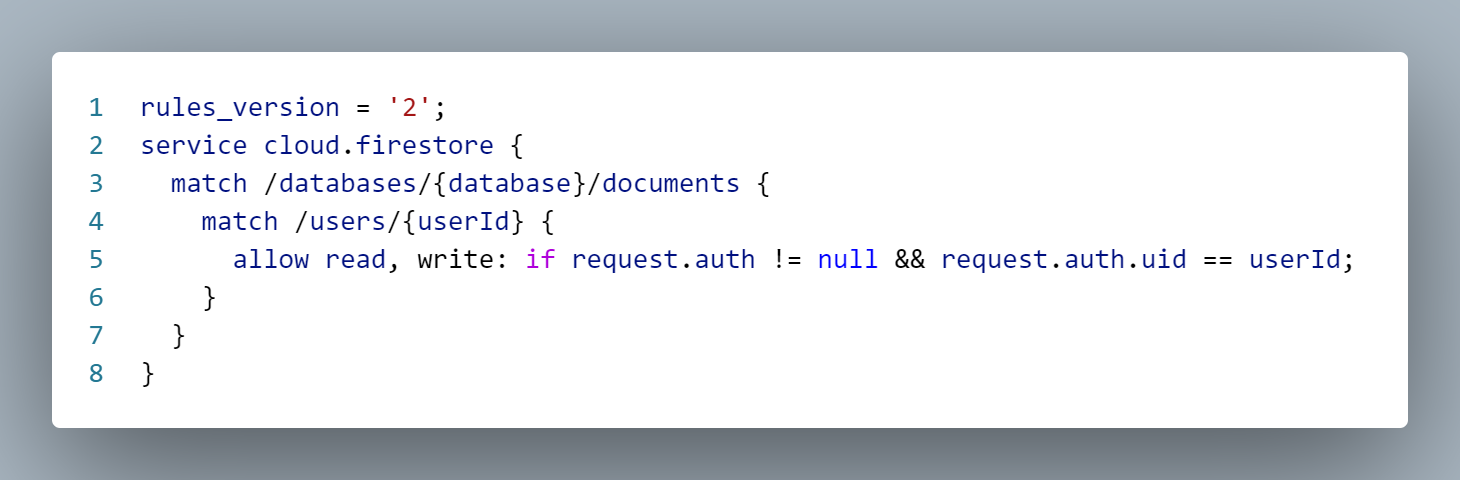
\includegraphics[width=\textwidth]{FireBaseRegla}
	\caption[Regla Firebase]{Regla definida en Firebase para el control de acceso a los datos.}
\end{figure}


\subsection{Blockchain}

Dentro de los contratos inteligentes los datos se estructuran utilizando estructuras y mapeos que facilitan la gestión y el acceso eficiente de la información. 

Los atributos del contrato recogidos en  \texttt{ContractDetails} incluyen:
\begin{itemize}
    \item \textbf{salary} (\texttt{uint256}): Salario acordado para el
 	 contrato, manejado en wei.
    \item \textbf{startDate} (\texttt{uint256}): Fecha de inicio del
     contrato representada en segundos.
    \item \textbf{duration} (\texttt{uint256}): Duración total del contrato
     en segundos.
    \item \textbf{title} (\texttt{string}): Título del contrato.
    \item \textbf{description} (\texttt{string}): Descripción del
     contrato.
    \item \textbf{isSigned} (\texttt{bool}): Estado que indica si el
     contrato ha sido firmado.
    \item \textbf{worker} (\texttt{address}): Dirección Ethereum del
     trabajador asignado al contrato.
    \item \textbf{isFinished} (\texttt{bool}): Estado que indica si el
     contrato ha concluido.
    \item \textbf{isReleased} (\texttt{bool}): Estado que señala si el pago
     ha sido liberado.
    \item \textbf{isPaused} (\texttt{bool}): Indica si el contrato está
     actualmente pausado.
    \item \textbf{pauseTime} (\texttt{uint256}): Tiempo en segundos que
     indica cuando el contrato fue pausado.
    \item \textbf{pauseDuration} (\texttt{uint256}): Acumulación de tiempo
     de pausas durante la ejecución del contrato en segundos.
\end{itemize}

La estructura \texttt{ChangeProposal} se utiliza para gestionar propuestas de cambio en el contrato y contiene los siguientes campos:
\begin{itemize}
    \item \textbf{newTitle} (\texttt{string}): Nuevo título propuesto para
     el contrato.
    \item \textbf{newSalary} (\texttt{uint256}): Nuevo salario propuesto,
     expresado en wei.
    \item \textbf{newDuration} (\texttt{uint256}): Nueva duración propuesta
     para el contrato, expresada en segundos.
    \item \textbf{newDescription} (\texttt{string}): Nueva descripción
     detallada propuesta para el contrato.
    \item \textbf{isPaused} (\texttt{bool}): Indica si la propuesta incluye
     una pausa del contrato.
    \item \textbf{isPending} (\texttt{bool}): Estado que indica si la
     propuesta está pendiente de aprobación.
\end{itemize}

En los contratos inteligentes, se usa mapeos y \textit{arrays} para organizar y relacionar de manera eficiente a los usuarios con los contratos.

\begin{itemize}

\item \textbf{mapping(uint256 => ContractDetails)}: almacena los datos de cada contrato mediante el \texttt{tokenId}, que es un identificador único.

\item \textbf{mapping(uint256 => ChangeProposal)}: almacena las propuestas de cambios en contratos mediante el \texttt{tokenId}, que es un identificador único.

\item \textbf{mapping(address => uint256[]) public contractsOwner}: relaciona cada empleador con una lista de \texttt{tokenIds} que representa los contratos que ha emitido.

\item \textbf{mapping(address => uint256[]) public activeContractsOfWorker}: Mantiene un registro de los contratos activos asignados a cada trabajador.

\item \textbf{mapping(address => uint256[]) public unsignedContractsOfWorker}: Lista los contratos que han sido ofrecidos a un trabajador pero que aún no han sido firmados.

\item \textbf{mapping(uint256 => address[]) public tokenManagersList}: Almacena una lista de direcciones que tienen permisos de gestión para un contrato.

\item \textbf{mapping(uint256 => mapping(address => bool)) public tokenManagers}: Determina qué direcciones tienen permisos de gestión sobre un contrato específico, facilitando la administración.

En la imagen \ref{img:EntidadRelacion} se puede observar el diagrama entidad-relación que muestra como las diferentes entidades se relacionan entre sí. 

\end{itemize}

\begin{figure}[h]
	\label{img:EntidadRelacion}
	\centering
	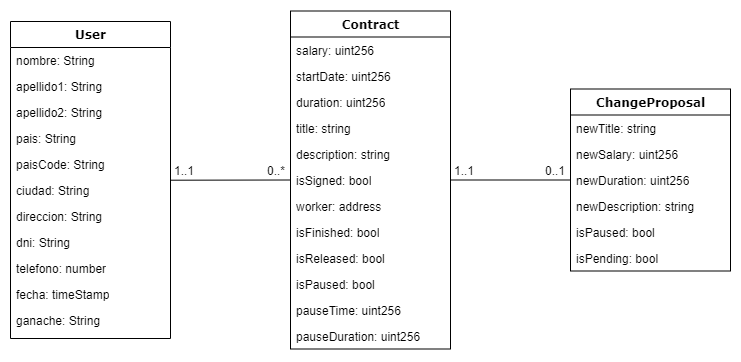
\includegraphics[width=\textwidth]{EntidadRelacion}
	\caption[Diagrama entidad-relación]{Diagrama entidad-relación.}
\end{figure}


\section{Diseño procedimental}

En esta sección se mostrarán los diagramas de secuencia de las dos tareas principales de la aplicación; crear un contrato (ver figura \ref{fig:SecuenciaCrearContrato}) y firmar un contrato (ver figura \ref{fig:SecuenciaFirmarContrato}).

\begin{figure}[h]
	\label{img:SecuenciaCrearContrato}
	\centering
	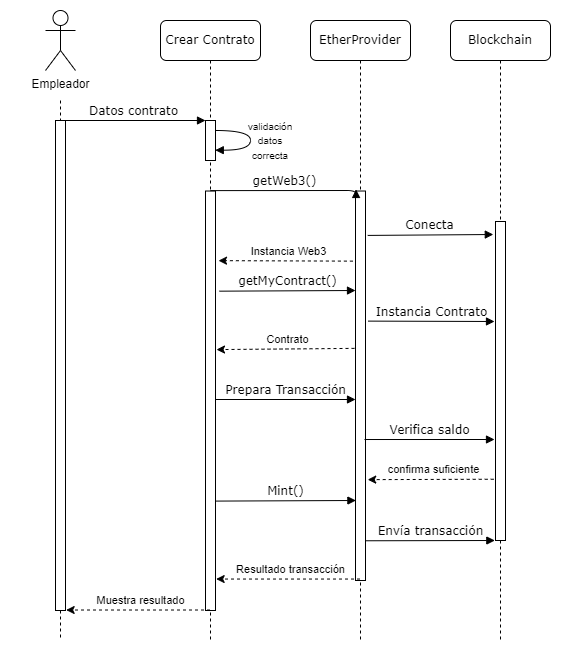
\includegraphics[width=\textwidth]{SecuenciaCrearContrato}
	\caption[Diagrama secuencia creación contrato]{Diagrama de secuencia para crear un contrato.}
\end{figure}

\begin{figure}[h]
	\label{img:SecuenciaFirmarContrato}
	\centering
	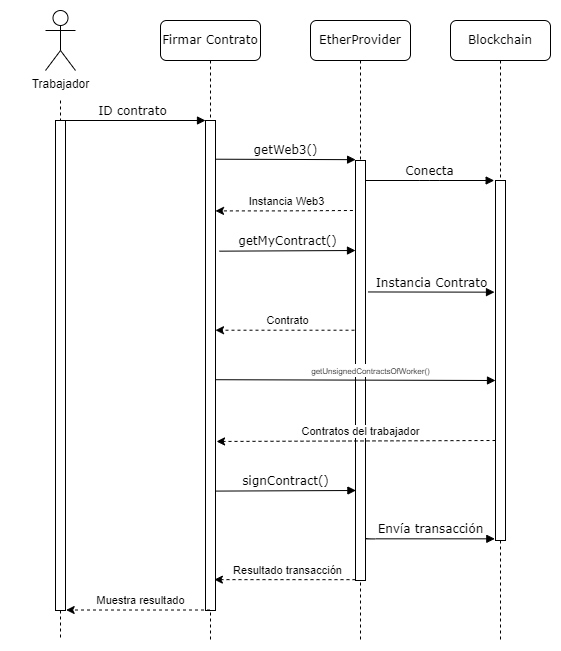
\includegraphics[width=\textwidth]{SecuenciaFirmarContrato}
	\caption[Diagrama secuencia firmar contrato]{Diagrama de secuencia para firmar un contrato.}
\end{figure}

\section{Diseño arquitectónico}

En este apartado se hablará de los patrones y estructuras que se han empleado en el proyecto.

\subsection{Estructura de la aplicación}

Antes de adentrarnos en los patrones de diseño específicos que estructuran el proyecto, es necesario comprender la arquitectura subyacente de la aplicación. 
Esta estructura no solo define la organización lógica y física de los componentes del software, sino que también establece las bases para un sistema robusto y escalable.

La aplicación está dividida en varios módulos principales, cada uno con responsabilidades claras y bien definidas. Esta separación facilita tanto el desarrollo como el mantenimiento. Además, tal estructura modular hace que el sistema sea más manejable y menos propenso a errores.

\subsection{Patrón Singleton}

El patrón Singleton es un diseño software que se utiliza para restringir la instanciación de una clase a un solo objeto. El patrón Singleton se implementa al crear una clase con un método que crea una nueva instancia de la clase si una no existe. En caso de que la instancia ya exista, simplemente devuelve una referencia a ese objeto.

En nuestro proyecto, el patrón Singleton se aplica en la clase \texttt{EtherProvider} (ver imagen \ref{img:singleton}) para manejar tanto la conexión a la \textit{blockchain} mediante Web3 como la instancia del contrato inteligente, garantizando que ambos sean únicos y globalmente accesibles.

\begin{figure}[h]
	\label{img:singleton}
	\centering
	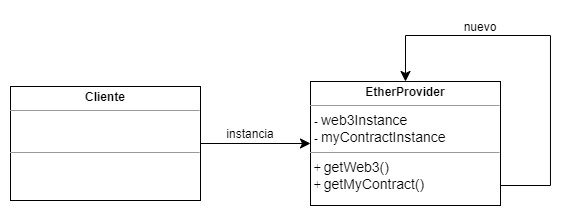
\includegraphics[width=\textwidth]{singleton}
	\caption[Diagrama Singleton]{Diagrama UML de la estructura del Singleton.}
\end{figure}

La implementación de patrón Singleton en el proyecto ofrece ventajas significativas: 

\begin{itemize}
\item \textbf{Eficiencia de recursos}: Solo se crea una instancia, ahorrando recursos y evitando la sobrecarga de establecer múltiples conexiones a la red.

\item \textbf{Consistencia}: Se mantiene una única conexión a lo largo de toda la aplicación, asegurando que todas las operaciones sobre la \textit{blockchain} se manejan de manera consistente.

\item \textbf{Gestión Centralizada}: Facilita la gestión y acceso a la red \textit{blockchain}, ya que los cambios en la conexión se manejan en un único lugar.
\end{itemize}

\subsection{Patrón Módulo}

El Patrón de Módulos es una pieza fundamental en la estructura de diseño y organización del código, permitiendo una clara división y encapsulación de funcionalidades dentro de la aplicación. Este patrón se manifiesta a través de la separación lógica de diferentes áreas de funcionalidad en directorios y archivos específicos, cada uno destinado a manejar distintos aspectos del sistema, facilitando así tanto el desarrollo como el mantenimiento de la aplicación.

Por ejemplo, la aplicación incluye directorios como \texttt{Contracts}, \texttt{components}, \texttt{Screens} o \texttt{AppLogin}, cada uno abordando un conjunto específico de responsabilidades dentro de la aplicación:

\begin{itemize}
\item \textbf{Contracts}: Gestiona toda la lógica relacionada con los contratos inteligentes.

\item \textbf{AppLogin}: Maneja la autenticación de usuarios.

\item \textbf{Components}: Contiene elementos de UI reutilizables como botones.

\item \textbf{Screens}: Encapsula los componentes de UI para cada pantalla de la aplicación.
\end{itemize}

Esta modularización asegura que los cambios dentro de un módulo específico puedan realizarse sin afectar a otras partes del sistema. Al mantener cada módulo independiente, se mejora significativamente la legibilidad y la mantenibilidad del código.

\section{Diseño de interfaces}

Antes del desarrollo de la interfaz de la aplicación, se experimentó y depuró un prototipo de la misma.
Las interfaces fueron diseñadas teniendo en cuenta la usabilidad de la aplicación, priorizando un diseño simple que permitiera que la aplicación fuera intuitiva, con una curva de aprendizaje suave.
También se ha considerado que la aplicación sea adaptable a una amplia variedad de pantallas, ya que puede ser utilizada tanto en dispositivos móviles como en tabletas.

El diseño de los prototipos para la aplicación incluye varias pantallas clave: pantalla de inicio de sesión, permitiendo la autenticación de los usuarios (ver imagen \ref{img:prototipoLogin}); la pantalla principal, que actúa como punto de entrada intuitivo (ver imagen \ref{img:prototipoHome}); la pantalla de creación de contratos, donde los usuarios pueden interactuar de manera clara y directa para establecer acuerdos(ver imagen \ref{img:prototipoCrearContrato}); la pantalla de visualización de contratos , diseñada para proporcionar una experiencia fluida al revisar contratos existentes (ver imagen \ref{img:prototipoVerContratos}); la pantalla de información y utilidades, que ofrece recursos y herramientas fácilmente accesibles (ver imagen \ref{img:prototipoInfo}); y la pantalla de estado de cuenta, que muestra de manera clara y concisa la información financiera relevante del usuario (ver imagen \ref{img:prototipoCartera}). 

\begin{figure}[h]
	\label{img:prototipoLogin}
	\centering
	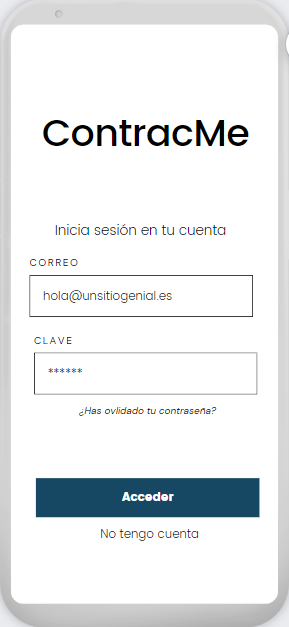
\includegraphics[width=0.40\textwidth]{prototipoLogin}
	\caption[Prototipo pantalla inicio de sesión]{Prototipo pantalla inicio de sesión.}
\end{figure}

\begin{figure}[h]
	\label{img:prototipoHome}
	\centering
	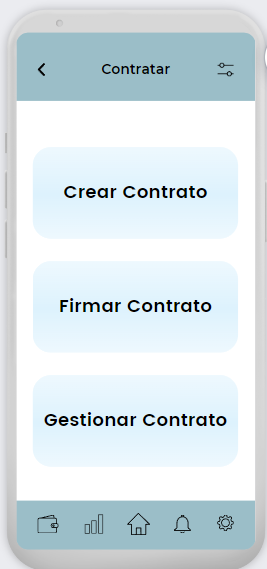
\includegraphics[width=0.40\textwidth]{prototipoHome}
	\caption[Prototipo pantalla principal]{Prototipo pantalla principal.}
\end{figure}

\begin{figure}[h]
	\label{img:prototipoCrearContrato}
	\centering
	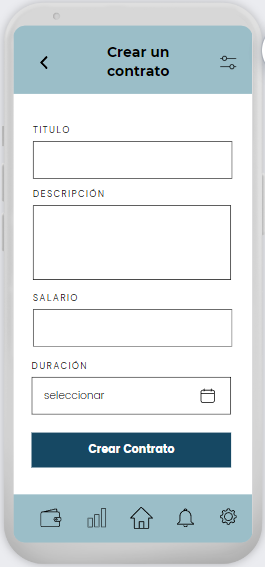
\includegraphics[width=0.40\textwidth]{prototipoCrearContrato}
	\caption[Prototipo pantalla crear contrato]{Prototipo pantalla crear contrato.}
\end{figure}

\begin{figure}[h]
	\label{img:prototipoVerContratos}
	\centering
	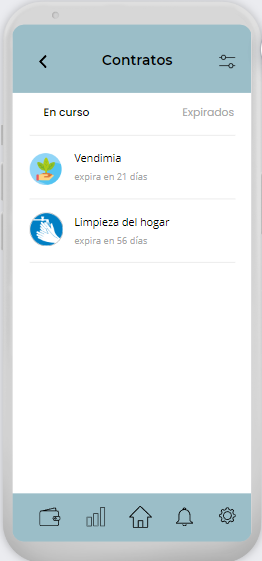
\includegraphics[width=0.40\textwidth]{prototipoVerContratos}
	\caption[Prototipo pantalla ver contratos del usuario]{Prototipo pantalla ver contratos del usuario.}
\end{figure}

\begin{figure}[h]
	\label{img:prototipoInfo}
	\centering
	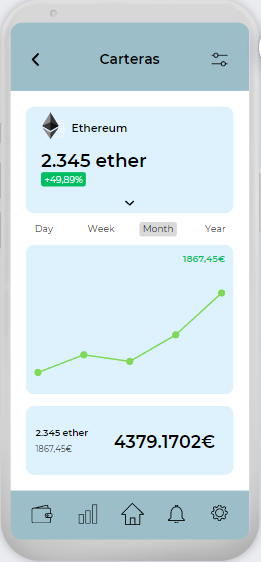
\includegraphics[width=0.40\textwidth]{prototipoInfo}
	\caption[Prototipo pantalla información y utilidades]{Prototipo pantalla información y utilidades.}
\end{figure}

\begin{figure}[h]
	\label{img:prototipoCartera}
	\centering
	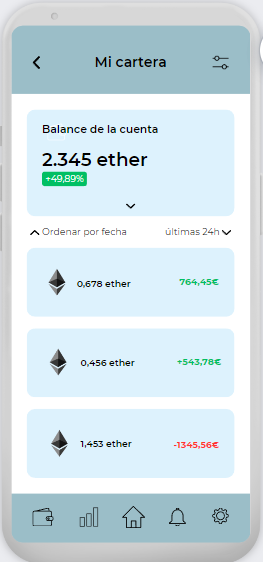
\includegraphics[width=0.40\textwidth]{prototipoCartera}
	\caption[Prototipo pantalla estado cuenta del usuario]{Prototipo pantalla estado cuenta del usuario.}
\end{figure}

\apendice{Documentación técnica de programación}

\section{Introducción}

En esta sección se describe la estructura del proyecto, el proceso de instalación y las herramientas necesarias para desarrollar el trabajo. También se explica cómo realizar la instalación de dependencias, la compilación, la ejecución del proyecto y el despliegue en Expo.

\section{Estructura de directorios}

En el primer nivel, se encuentran dos directorios, \textbf{Documentacion} y \textbf{Code}. El primero de ellos recoge los archivos de documentación sobre el proyecto, como la memoria y sus anexos, por otra parte, el segundo recoge la lógica de la aplicación.

Dentro de Code, el directorio \textbf{AppContractMe} contiene todo el código fuente necesario para la interfaz de usuario de la aplicación. Se divide en varios subdirectorios que organizan los recursos y \textit{scripts} de manera lógica, siendo \textbf{scr} el más importante, incluyendo:

\begin{itemize}

\item \textbf{AppLogin:} Contiene los componentes para la autenticación y gestión de sesiones de usuario.

\item \textbf{ContractConexion:} Incluye las funciones que facilitan la conexión y la interacción con los contratos inteligentes.

\item \textbf{Screens:} Agrupa las diferentes pantallas de la aplicación, permitiendo la navegación al usuario.

\item \textbf{components:} Reúne elementos reutilizables que se emplean en diversas partes de la aplicación, como botones y ciertas funcionalidades.

\end{itemize}

Por otro lado, también existe el directorio \textbf{SmartContract} que recoge toda la lógica del contrato inteligente e incluye:

\begin{itemize}

\item \textbf{build:} Contiene los archivos compilados de los contratos, que son necesarios para su despliegue y ejecución en la \textit{blockchain}.

\item \textbf{constracts:} Alberga los \textit{scripts} de los contratos inteligentes.

\item \textbf{migrations:} Gestiona el \textit{scripts} que ayuda en la migración y despliegue de los contratos en la \textit{blockchain}.

\item \textbf{node\_modules:} Directorio que incluye las dependencias de \texttt{Node.js} utilizadas en el proyecto.

\item \textbf{test:} Contiene los \textit{test} escritos en java para asegurar el correcto funcionamiento de los contratos inteligentes.

\end{itemize}

Finalmente hay otro directorio llamada \textbf{ganache\_db} el cual se utiliza para almacenar la configuración y los datos de la base de datos de Ganache.

Toda la jerarquía de la aplicación se puede observar en la imagen \ref{img:FolderTree}.

\begin{figure}[h]
	\label{img:FolderTree}
	\centering
	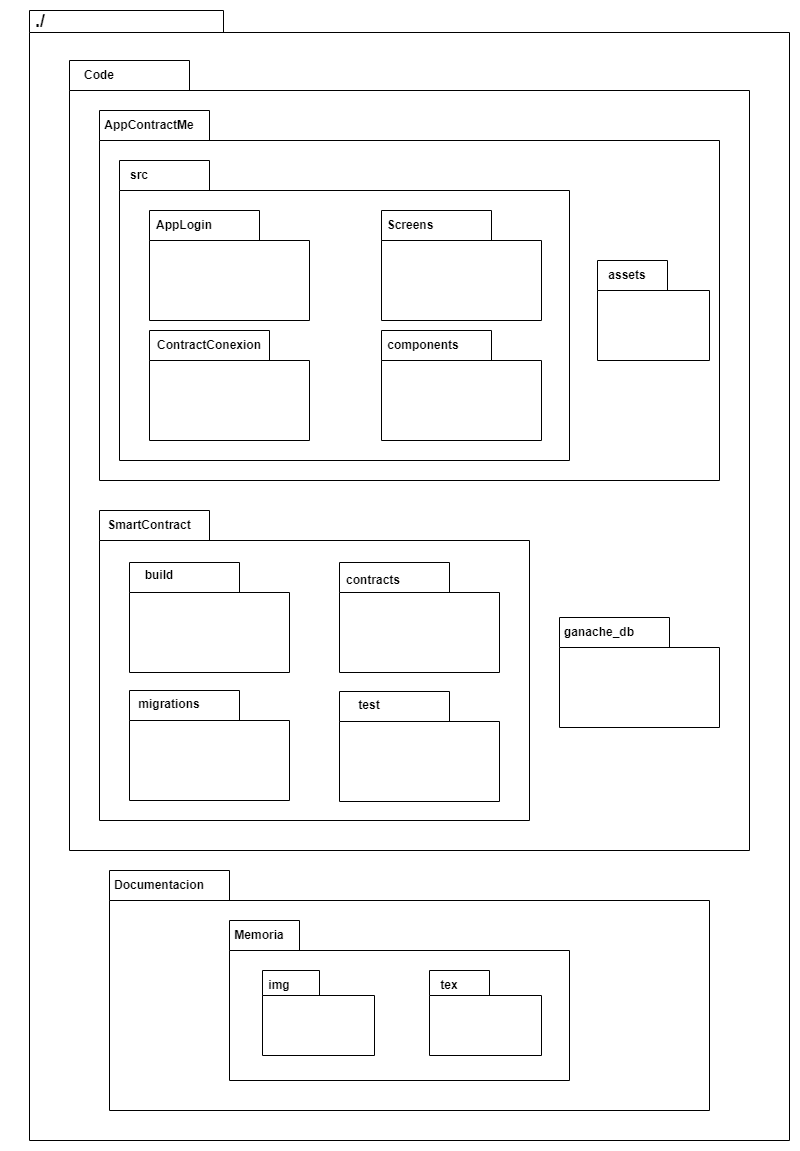
\includegraphics[width=\textwidth]{FolderTree}
	\caption[Directorios del proyecto]{Directorios del proyecto.}
\end{figure}


\section{Manual del programador}

Este apartado servirá de ayuda y referencia a futuros desarrolladores que quieran replicar el proyecto. 
Por ello se detallará los requisitos necesarios y el proceso de instalación para el desarrollo de la aplicación. 

\subsection{Entorno desarrollo}

Antes de explicar la instalación de los programas y herramientas para el desarrollo de la aplicación es necesario detallar unas especificaciones mínimas en cuanto al equipo de desarrollo para poder trabajar con el proyecto.

\begin{enumerate}

\item\textbf{Procesador (CPU):}
	\begin{itemize}
	\item\textbf{Mínimo:} Procesador con arquitectura x86\_64, 2º generación de Intel o procesador AMD que
	 soporte `Hypervisor FrameWork', Permitiendo una compilación rápida de código y emular un dispositivo 	
	 móvil para pruebas.
	\item\textbf{Recomendado:} Intel Core i7 o AMD ryzen 7, con 6-8 núcleos.
	\end{itemize}
	
\item\textbf{Memoria RAM:}
	\begin{itemize}
	\item\textbf{Mínimo:} 8 GB de RAM como mínimo, para manejar diversas tareas y la ejecución de
	simuladores.
	\item\textbf{Recomendado:} 16 GB de RAM o más, pudiendo mantener múltiples dispositivos emulados
	simultáneamente.
	\end{itemize}
	
\item\textbf{Sistema operativo:}
	\begin{itemize}
	\item\textbf{Mínimo:} Windows 10 64-bit.
	\item\textbf{Recomendado:} Windows 11.
	\end{itemize}

\end{enumerate}

Por otro lado, aunque no es un requisito obligatorio, se recomienda contar con un dispositivo Android físico para ejecutar la aplicación y hacer uso de funcionalidades nativas como el reconocimiento de huella, siendo necesario las siguientes especificaciones.

\begin{enumerate}

\item\textbf{Versión Android:}
	\begin{itemize}
	\item\textbf{Mínimo:}  Android 6.0 (Marshmallow)
	\item\textbf{Recomendado:} Android 9.0 (Pie) o superior.
	\end{itemize}
	
\item\textbf{Procesador (CPU):}
	\begin{itemize}
	\item\textbf{Mínimo:} Quad-core 1.2 GHz.
	\item\textbf{Recomendado:} Octa-core 2.0 GHz o superior.
	\end{itemize}
	
\item\textbf{RAM:}
	\begin{itemize}
	\item\textbf{Mínimo:} 2 GB de RAM.
	\item\textbf{Recomendado:} 4-8 GB de RAM.
	\end{itemize}
	
\item\textbf{Compatibilidad con características nativas:}
	\begin{itemize}
	\item\textbf{Huella digital:} El dispositivo debe contar con un sensor de huellas dactilares compatible con
	las API de Android para autenticación biométrica.
	\item\textbf{Reconocimiento facial:} cámara interior con capacidad de reconocimiento facial.
	\item\textbf{Cámara trasera:} Cámara de al menos 8 MP para la lectura de códigos QR.
	\end{itemize}

\end{enumerate}


\section{Compilación, instalación y ejecución del proyecto}
\label{instalacionProyecto}

\subsection{Instalación}

Seguidamente se detallará como configurar un entorno de desarrollo para poder trabajar en la aplicación ContractMe.

\begin{enumerate}

\item \textbf{Node.js:} Node.js es una plataforma de ejecución para JavaScript del lado del servidor y es esencial para la gestión de paquetes y la ejecución de varias herramientas de desarrollo. 
Para instalar Node.js es necesario dirigirse a la \href{https://nodejs.org/en}{pagina oficial de Node.js} y seleccionar el instalador para Windows. Ver imagen \ref{fig:InstalarNodejs}.

Al ejecutar el instalador que se ha descargado, es necesario seleccionar la opción que permite instalar npm y añadir Node.js a tu \textit{path}. Ver imagen \ref{fig:NodejsSetUp}.  
En concreto la versión utilizada de Node.js para el desarrollo del proyecto ha sido la v18.18.2 y la versión utilizada de npm ha sido la 10.2.2.

\begin{figure}[h]
	\label{img:InstalarNodejs}
	\centering
	\includegraphics[width=\textwidth]{InstalarNodejs}
	\caption[Descarga de Node.js]{Descarga de Node.js.}
\end{figure}

\begin{figure}[h]
	\label{img:NodejsSetUp}
	\centering
	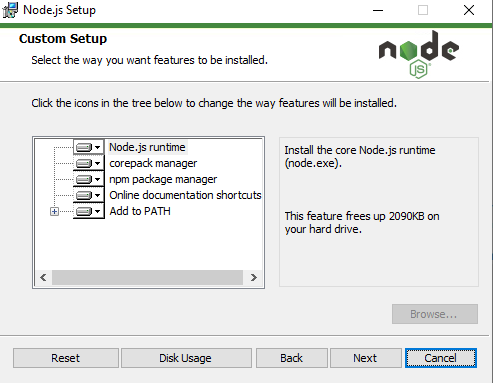
\includegraphics[width=\textwidth]{NodejsSetUp}
	\caption[Instalar Node.js y npm]{Instalar Node.js y npm.}
\end{figure}

\item \textbf{Truffle Suite}: Teniendo Node.js y npm instalados, procederemos a instalar Truffle globalmente, para ello desde la terminal ejecutaremos el siguiente comando: \texttt{npm install -g truffle} lo cual nos permitirá usar el comando \texttt{truffle} desde cualquier lugar en la terminal.

Una vez instalado Truffle, el siguiente paso es configurar el proyecto, para ello dentro del directorio \textit{Smart Contract}, se encuentra la estructura de carpetas generadas por Truffle, incluyendo \textit{contracts} para almacenar la lógica de los contratos, \textit{migrations} para almacenar el \textit{migrations} de migración y \textit{test} para las pruebas.

Truffle también crea un archivo de configuración llamado \texttt{truffle-config.js}, el cual se usa para configurar las redes sobre las cuales se desplegarán los contratos inteligentes.
En este caso se usa la red de Ganache, que normalmente se ejecuta en \texttt{localhost} en el ordenador. Debido a que la aplicación se ejecutará en un dispositivo móvil independiente del ordenador, la configuración \textit{localhost} no será suficiente. 
En su lugar, se usará la dirección IP del ordenador la cual actuará como servidor para Ganache. Esto permitirá que otros dispositivos de nuestra misma red local se conecten a la \textit{blockchain} simulada por Ganache.
Ganache por defecto usa el puerto 8545, aunque este podría ser reemplazado por cualquier puerto que se encontrase vacío.
Siguiendo los pasos previamente mencionados, el archivo \texttt{truffle-config.js} debería verse como en la imagen \ref{fig:TruffleGanache}.

\begin{figure}[h]
	\label{img:TruffleGanache}
	\centering
	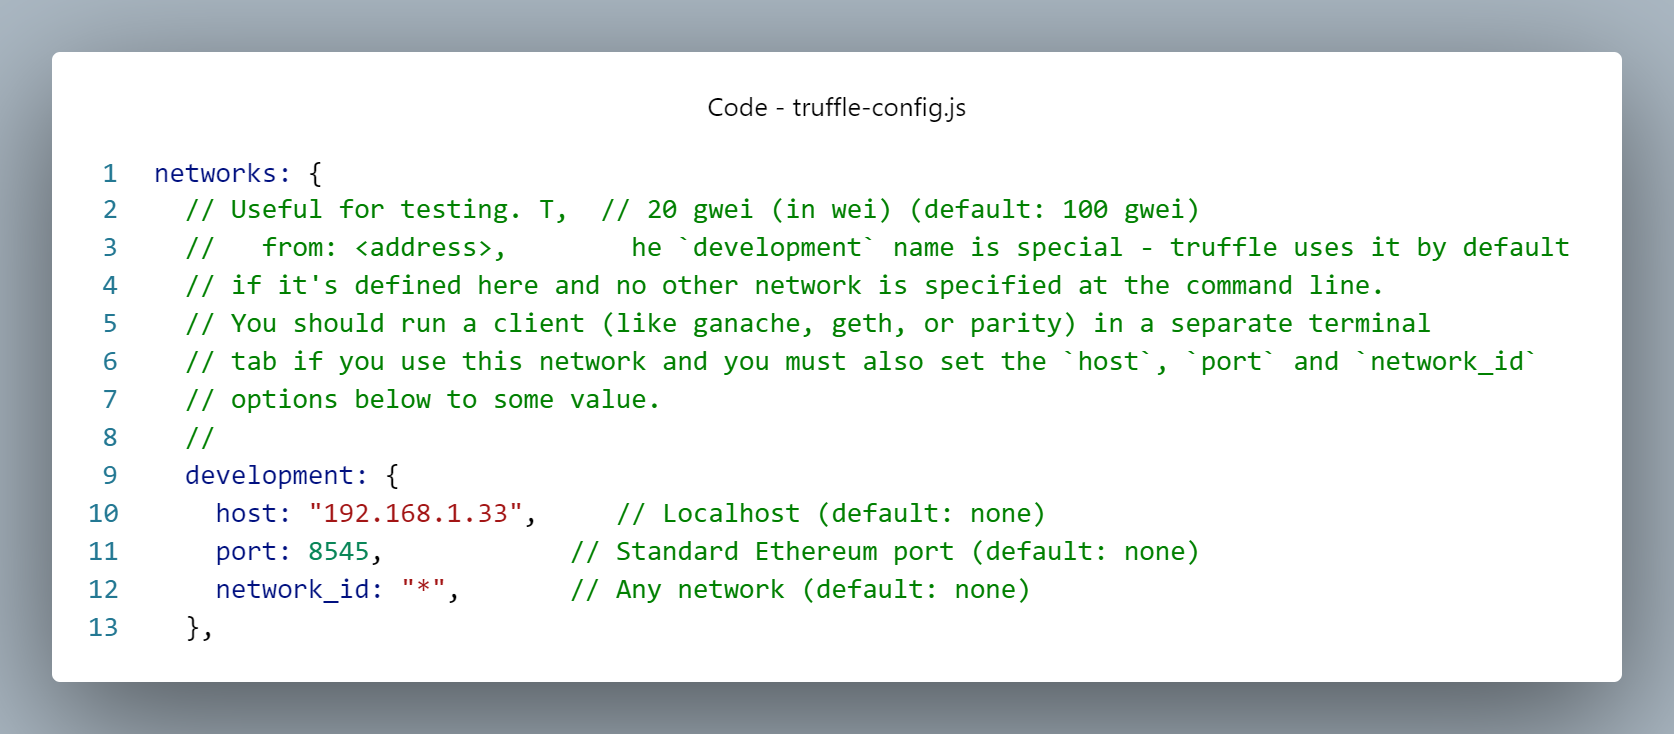
\includegraphics[width=\textwidth]{TruffleGanache}
	\caption[Configuración Ganache Truffle]{Configuración red Ganache en truffle-config.js.}
\end{figure}

Dentro del archivo \texttt{truffle-config.js} también será necesario realizar la configuración de compiladores para especificar como los contratos inteligentes deben de ser compilados, optimizados y ejecutados en la máquina virtual de Ethereum.
Se deberá especificar la versión \textbf{0.8.20}, la cual usará Truffle para compilar los contratos, esta versión coincide con la versión que se ha usado de Solidity para desarrollar los contratos inteligentes.
Dentro de \textit{Settings} se ha de especificar algunas opciones que afectan a la compilación de los contratos. La opción \textit{optimizer} debe marcarse como \textit{true}, ayudándonos a reducir el código \textit{byte} de los contratos y hacerlos más eficientes en términos de gas.
Por otro lado, las \textit{runs} se deben de establecer en 200, un número más alto puede resultar en un código más optimizado en términos de gas, pero con un proceso de compilación más lento. ver imagen \ref{fig:TruffleCompiler}.

\begin{figure}[h]
	\label{img:TruffleCompiler}
	\centering
	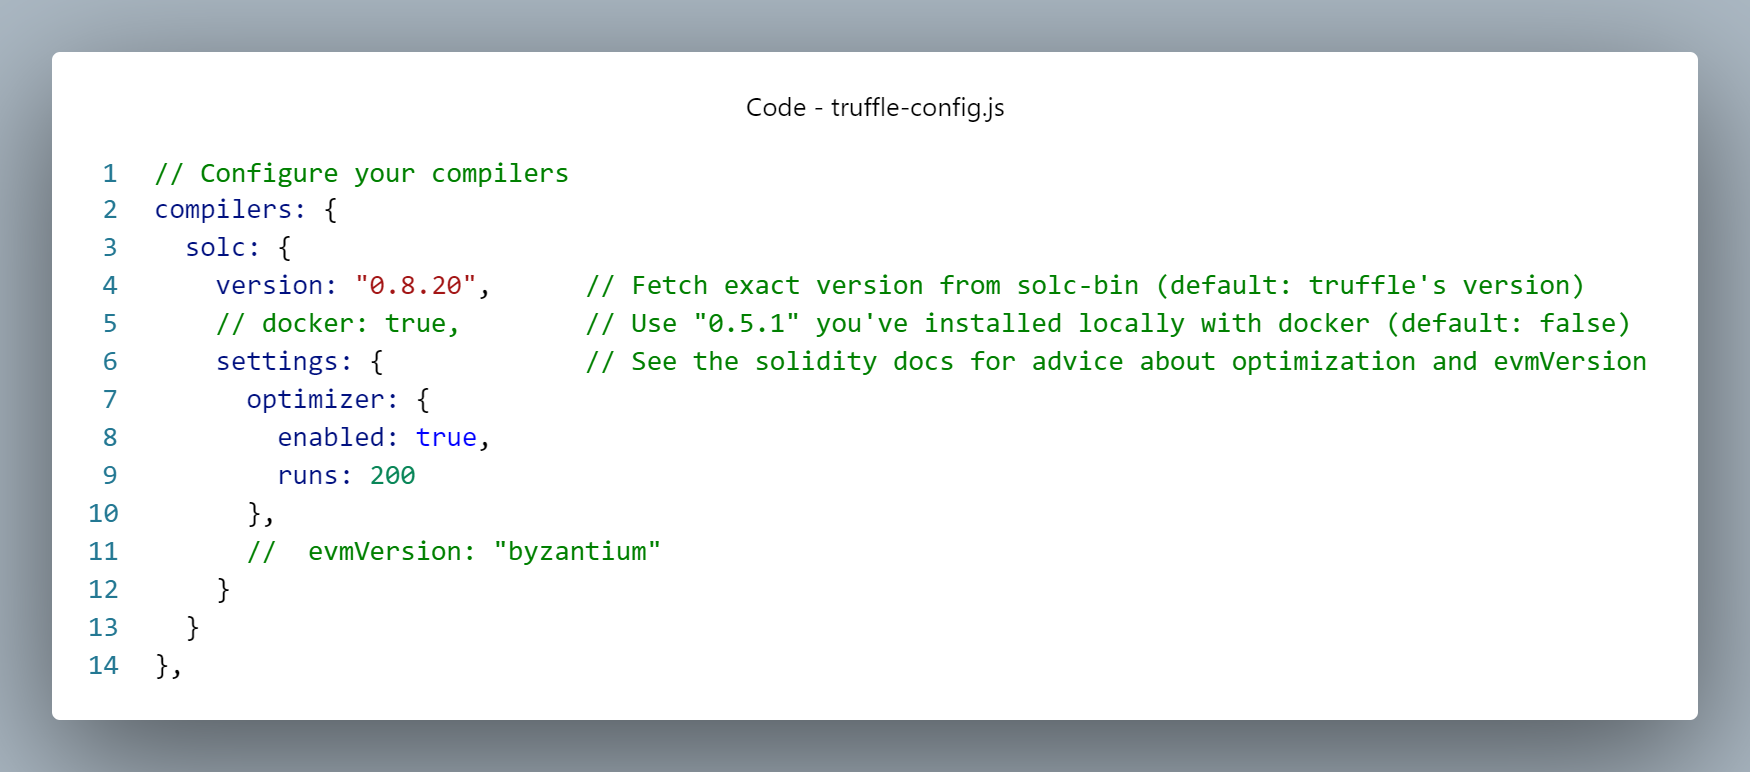
\includegraphics[width=\textwidth]{TruffleCompiler}
	\caption[Configuración compilador Truffle]{Configuración del compilador en truffle-config.js.}
\end{figure}

\item \textbf{Ganache}: Como hemos comentado, en el proyecto se usa la red de Ganache. Por simplicidad hemos usado la versión de consola, por tanto para instalarla de forma global en nuestro ordenador será necesario ejecutar el siguiente comando: \texttt{npm install -g ganache-cli}.

\item \textbf{Expo CLI}: Del mismo modo que hemos realizado con Ganache, previamente es necesario descargar Expo CLI, el cual es necesario para iniciar, desarrollar y probar el proyecto.
Utilizando el comando \texttt{npm install -g expo-cli} lo descargamos globalmente.

\item \textbf{Expo Go}: Para visualizar la aplicación se usará Expo Go permitiéndonos ejecutar la aplicación directamente en nuestra dispositivo móvil.
Para ello, desde el un dispositivo móvil Android utilizando Google Play Store, se buscará en la barra de búsqueda `Expo Go'.  Seguidamente se procederá a descargar dicha aplicación.

\item \textbf{Descarga del repositorio}: Para adquirir el código fuente del proyecto \href{https://gitlab.com/HP-SCDS/Observatorio/2023-2024/contractme/ubu-contractme.git}{`ContracMe'}, se puede descargar de utilizando la interfaz gráfica de GitLab descargando el fichero ZIP o usando \texttt{git clone} desde la terminal.

\end{enumerate}


\subsection{Ejecución del proyecto}

En este apartado se detallará como ejecutar el proyecto. Es muy importante que durante la ejecución tanto el ordenador como el dispositivo móvil se encuentren en la misma red.

\begin{enumerate}

\item \textbf{Levantar Ganache}: Antes de proceder a ejecutar la aplicación es necesario que la red Ganache se encuentre previamente en funcionamiento.
Como hemos comentado anteriormente, la red debe de ser levantada sobre la dirección IP local de nuestro ordenador. Por ejemplo, suponiendo que la IP local de mi ordenador es 192.168.1.33, deberemos de ejecutar desde cualquier parte de la terminal, el siguiente comando: 
\begin{verbatim}
ganache-cli --host 192.168.1.33 -d --db ganache_db
\end{verbatim}

\texttt{-d} es una abreviatura de deterministic, lo que hace que Ganache genere las mismas cuentas y claves privadas cada vez que se ejecuta.
\texttt{--db ganache\_db} es una opción que permite que Ganache guarde el estado de la red en un directorio específico, en este caso el directorio será llamado `ganache\_db' y se creará en la rama actual donde se encuentre el usuario en la terminal.
Esto permite que la \textit{blockchain} simulada mantenga su estado entre reinicios de Ganache.

En la imagen \ref{img:ganache-cli} se muestra el resultado de levantar exitosamente una red Ganache desde la terminal.

\begin{figure}[h]
	\label{img:ganache-cli}
	\centering
	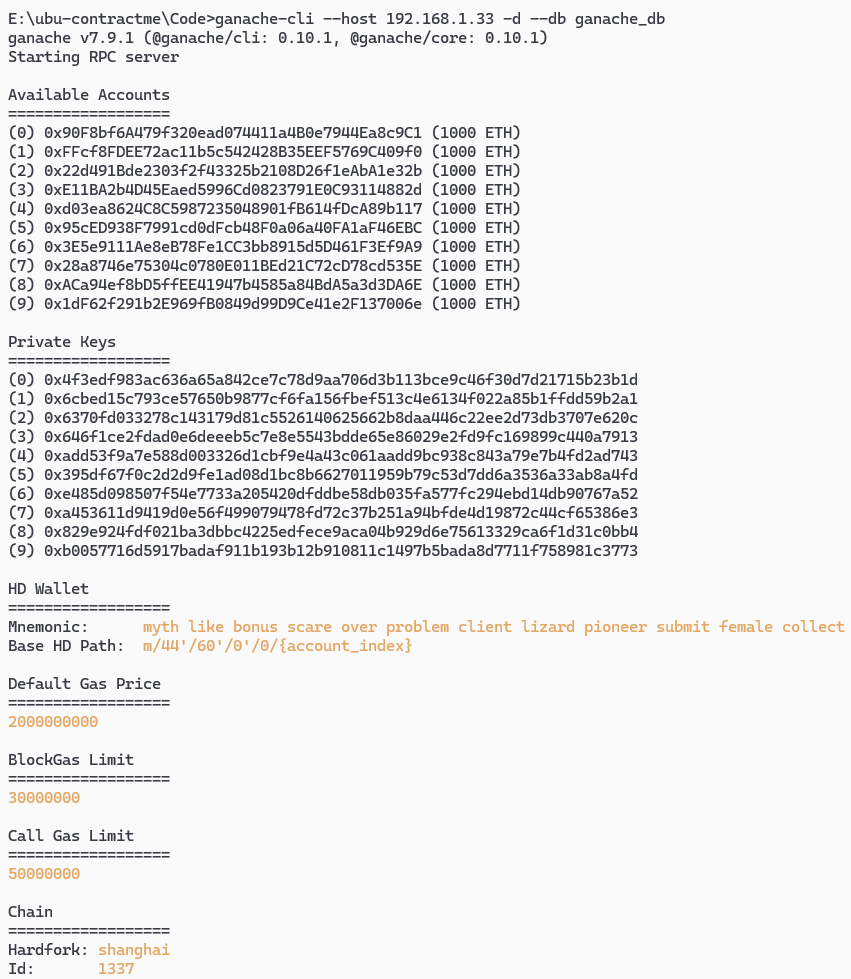
\includegraphics[width=\textwidth]{ganache-cli}
	\caption[Levantar red Ganache]{Levantar red local usando Ganache.}
\end{figure}

\item \textbf{Compilar y migrar contrato}: el contrato debe de ser compilado, probado y migrado antes de poder utilizarlo, para ello se utiliza Truffle.

	\begin{itemize}
	\item \textbf{Compilar}: Es necesario convertir el código
	Solidity de los contratos en \textit{bytecode} que pueda
	ser ejecutado por la Máquina Virtual de Ethereum (EVM).
	Para ello desde el directorio \textit{SmartContract} donde se
	almacena toda la lógica de los contratos
	inteligentes, se debe ejecutar el comando \texttt{truffle
	compile}.
	Ver imagen \ref{img:TruffleCompiler}.
	\end{itemize}
	
\begin{figure}[h]
	\label{img:TruffleCompile}
	\centering
	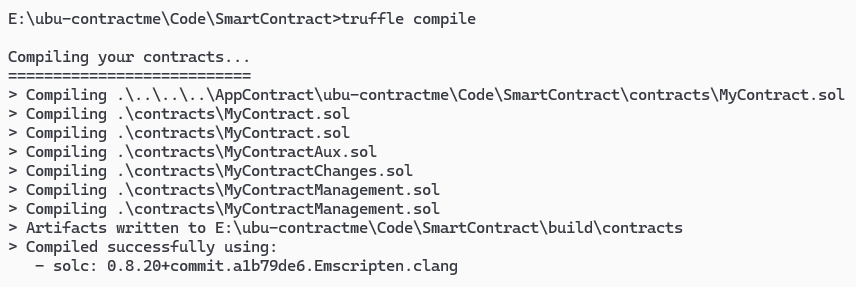
\includegraphics[width=\textwidth]{TruffleCompile}
	\caption[Compilar smart contract]{Compilar \textit{cmart contract} usando Truffle.}
\end{figure}	
	
	\begin{itemize}
	\item \textbf{Migrar}: Finalmente, el último paso es desplegar el contrato en la \textit{blockchain}.
	Esto se realiza desde el directorio \texttt{SmartContract} usando el comando \texttt{truffle migrate}.
	Este comando desplegará los contratos inteligentes en la red configurada, en este caso Ganache y generará
	los archivos necesarios en el directorio \texttt{build/contracts}.
	Tras una correcta migración, se mostrará la dirección del contrato, la cuenta del creador, el costo total
	del despliegue, etcétera. 	
Ver imagen \ref{img:TruffleMigrate}.
	\end{itemize}
	
\begin{figure}[h]
	\label{img:TruffleMigrate}
	\centering
	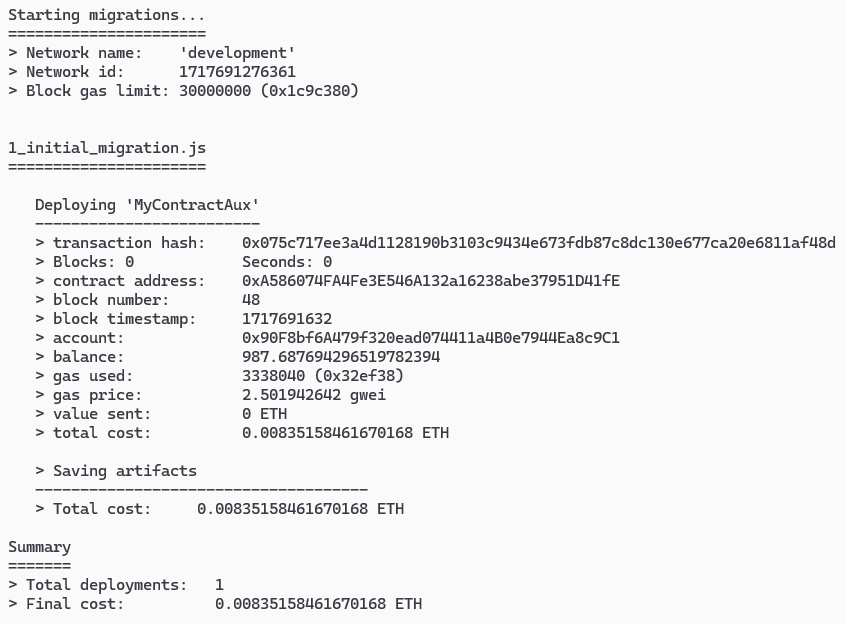
\includegraphics[width=\textwidth]{TruffleMigrate}
	\caption[Despliegue smart contract]{Despliegue del contrato en la red de Ganache usando Truffle.}
\end{figure}	
	
	
\item \textbf{Configuración conexión contrato}: Una vez hayamos desplegado un nuevo contrato en la \textit{blockchain}, debemos actualizar la información de la aplicación para que esta pueda interactuar con él.
Para ello, necesitamos dos cosas: la dirección del contrato, que se nos ha proporcionado en la terminal al migrarlo, y el archivo JSON del contrato que se encuentra en \texttt{SmartContract/build}.
	
Con el archivo JSON del contrato, es necesario copiarlo y pegarlo en la carpeta \texttt{AppContract/src/ContractConexion}. 
Por otro lado con la dirección del contrato, también es necesario copiarla, y actualizar la referencia \texttt{contractAddress} que se encuentra en el archivo \texttt{EtherProvider.js}.
Ver imagen \ref{img:ContractConexion}.

\begin{figure}[h]
	\label{img:ContractConexion}
	\centering
	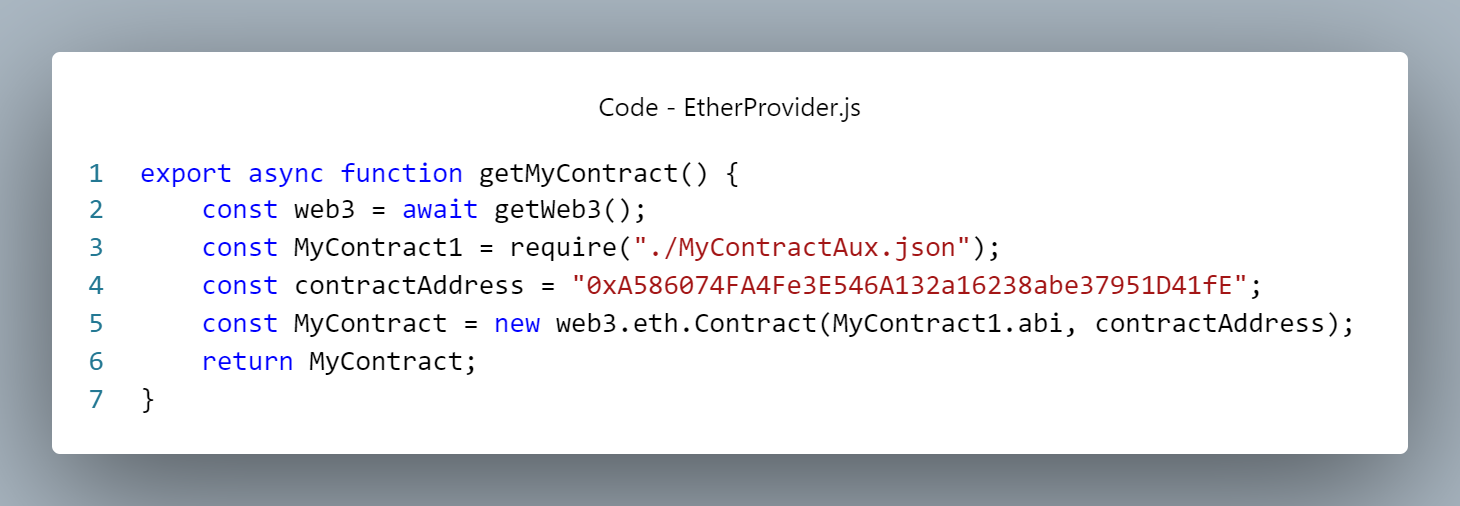
\includegraphics[width=\textwidth]{ContractConexion}
	\caption[Conexión con el contrato]{Configuración de conexión con el contrato.}
\end{figure}	

\item \textbf{Iniciar aplicación}: Desde el directorio raíz de la aplicación, \texttt{/Code/AppContract}, en la terminal ejecutamos el comando \texttt{npx expo start} para iniciar el servidor. Esto mostrará un código QR en la terminal. Será necesario comprobar que la opción Expo Go se encuentre activa.
Seguidamente desde la aplicación Expo Go en el dispositivo móvil, se procederá a escanear el código QR que aparece en la terminal.
La aplicación Expo Go cargará y mostrará la aplicación en el dispositivo móvil.

\end{enumerate}

\section{Pruebas del sistema}

\begin{itemize}

\item \textbf{Probar}: Como paso opcional, pero altamente recomendado, para comprobar el correcto funcionamiento del contrato, se puede ejecutar una batería de \textit{test}. Estos \textit{tests} están diseñados para asegurar que todas las funciones del contrato inteligente operen conforme a las especificaciones establecidas y para identificar cualquier posible falla antes de la implementación en un entorno de producción.
	
\item \textbf{Proceso de ejecución de pruebas}: Para llevar a cabo estas pruebas unitarias, es necesario utilizar el comando \texttt{truffle test} en la terminal. Este comando debe ejecutarse desde el directorio \textit{Smart Contract}, donde se encuentran almacenados todos los \textit{scripts} de prueba necesarios para la evaluación del contrato.

\item \textbf{Descripción de los \textit{tesst}}: 
Los \textit{tests} verifican cada función y transacción que el
contrato inteligente puede realizar, incluyendo la creación,
transferencia y administración de los contratos.
Cada \textit{test} está diseñado para garantizar que el contrato responda adecuadamente en cualquier situación.

\item \textbf{Interpretación de resultados}: Al finalizar la ejecución de los \textit{test}, \texttt{truffle} proporcionará un reporte detallado que incluirá el resultado de cada prueba individual.
Un \textit{test} exitoso indica que la función correspondiente del contrato cumple con los requisitos y funciona como se espera. 
Para ver un ejemplo de cómo se presentan estos resultados, ver la imagen \ref{fig:TruffleTest}.

\end{itemize}

\begin{figure}[h]
	\label{img:TruffleTest}
	\centering
	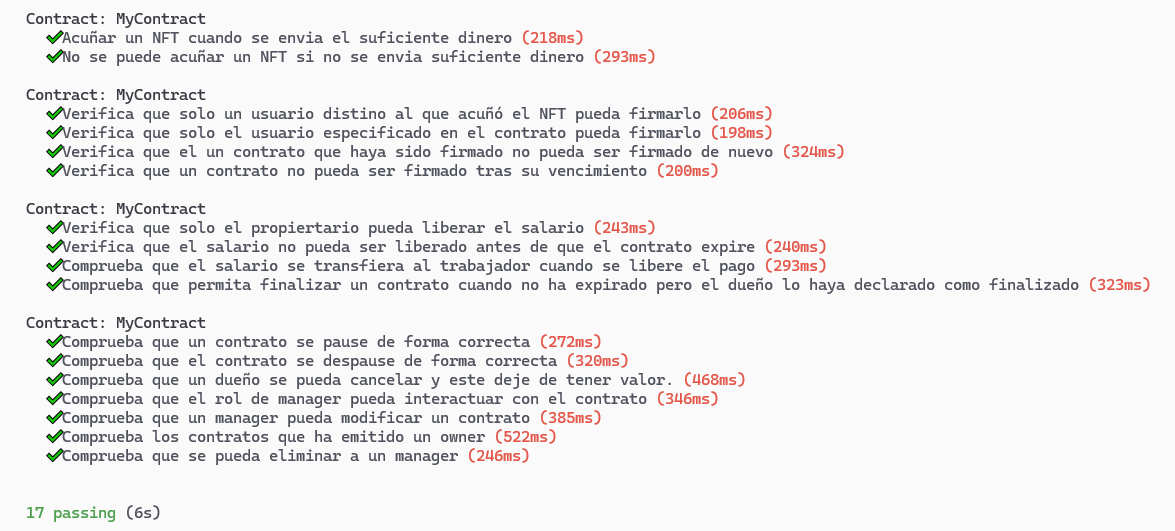
\includegraphics[width=\textwidth]{TruffleTest}
	\caption[Pruebas sobre el contrato]{Pruebas unitarias sobre el Smart Contract usando Truffle.}
\end{figure}	


\apendice{Documentación de usuario}

\section{Introducción}

En este apartado se describirán los requisitos y directrices para que los nuevos usuarios sean capaces de entrar en la aplicación y usarla efectivamente.

\section{Requisitos de usuarios}

Para utilizar la aplicación, es esencial que el usuario tenga instalados en su ordenador Ganache y Expo. 
Por otro lado, el usuario debe de tener instalada la aplicación Expo Go en su teléfono móvil y es recomendable que el dispositivo esté equipado con cámara, así como con sistemas de autenticación biométrica, como huella digital o reconocimiento facial. 
Además, es necesario que el teléfono móvil esté conectado a la misma red que el ordenador donde se ejecutan Ganache y Expo.

\section{Instalación}

El proceso de instalación del proyecto se describe más detalladamente en la sección `Manual del programador'.
Se puede resumir en:

\begin{enumerate}

\item Clonar el repositorio.

\item Ir a \textbf{Code/AppContractMe/src/ContractConexion/EtherProvider.js} y sustituir la variable `Url' por la IP de tu ordenador.

\item Desde el directorio \textbf{Code/AppContractMe} ejecutar \textbf{npx expo install} para descargar todas las dependencias.

\item ejecutar el comando \textbf{ganache --host \textit{tu\_ip} } desde cualquier lado en la terminal.

\item Desde el directorio \textbf{Code/AppContractMe} ejecutar \texttt{npx expo start}

\item Asegurándose de que nos encontremos en la opción `Expo Go', desde la aplicación Expo en tu teléfono móvil escanear el código QR.

\end{enumerate}

\section{Manual del usuario}

A continuación se procede a ilustrar las funcionalidades básicas de la aplicación. Es destacable comentar que para poder interactuar con todas la funcionalidades de la aplicación serán necesarias dos cuentas, una que ejerza como empleador y otra que ejerza como trabajador. Por lo que será necesario cerrar sesión y volver a abrirla con una cuenta diferente o usar dos dispositivos móviles simultáneamente.

\subsection{Identificación del usuario}

El primer paso para utilizar \textit{ContractMe}, es iniciar sesión para acceder a todas las funcionalidades de la misma. Es obligatorio rellenar tanto el campo de usuario (email) como el de la contraseña.
Ver imagen \ref{fig:inicioSesion}.

\begin{figure}[h]
	\centering
	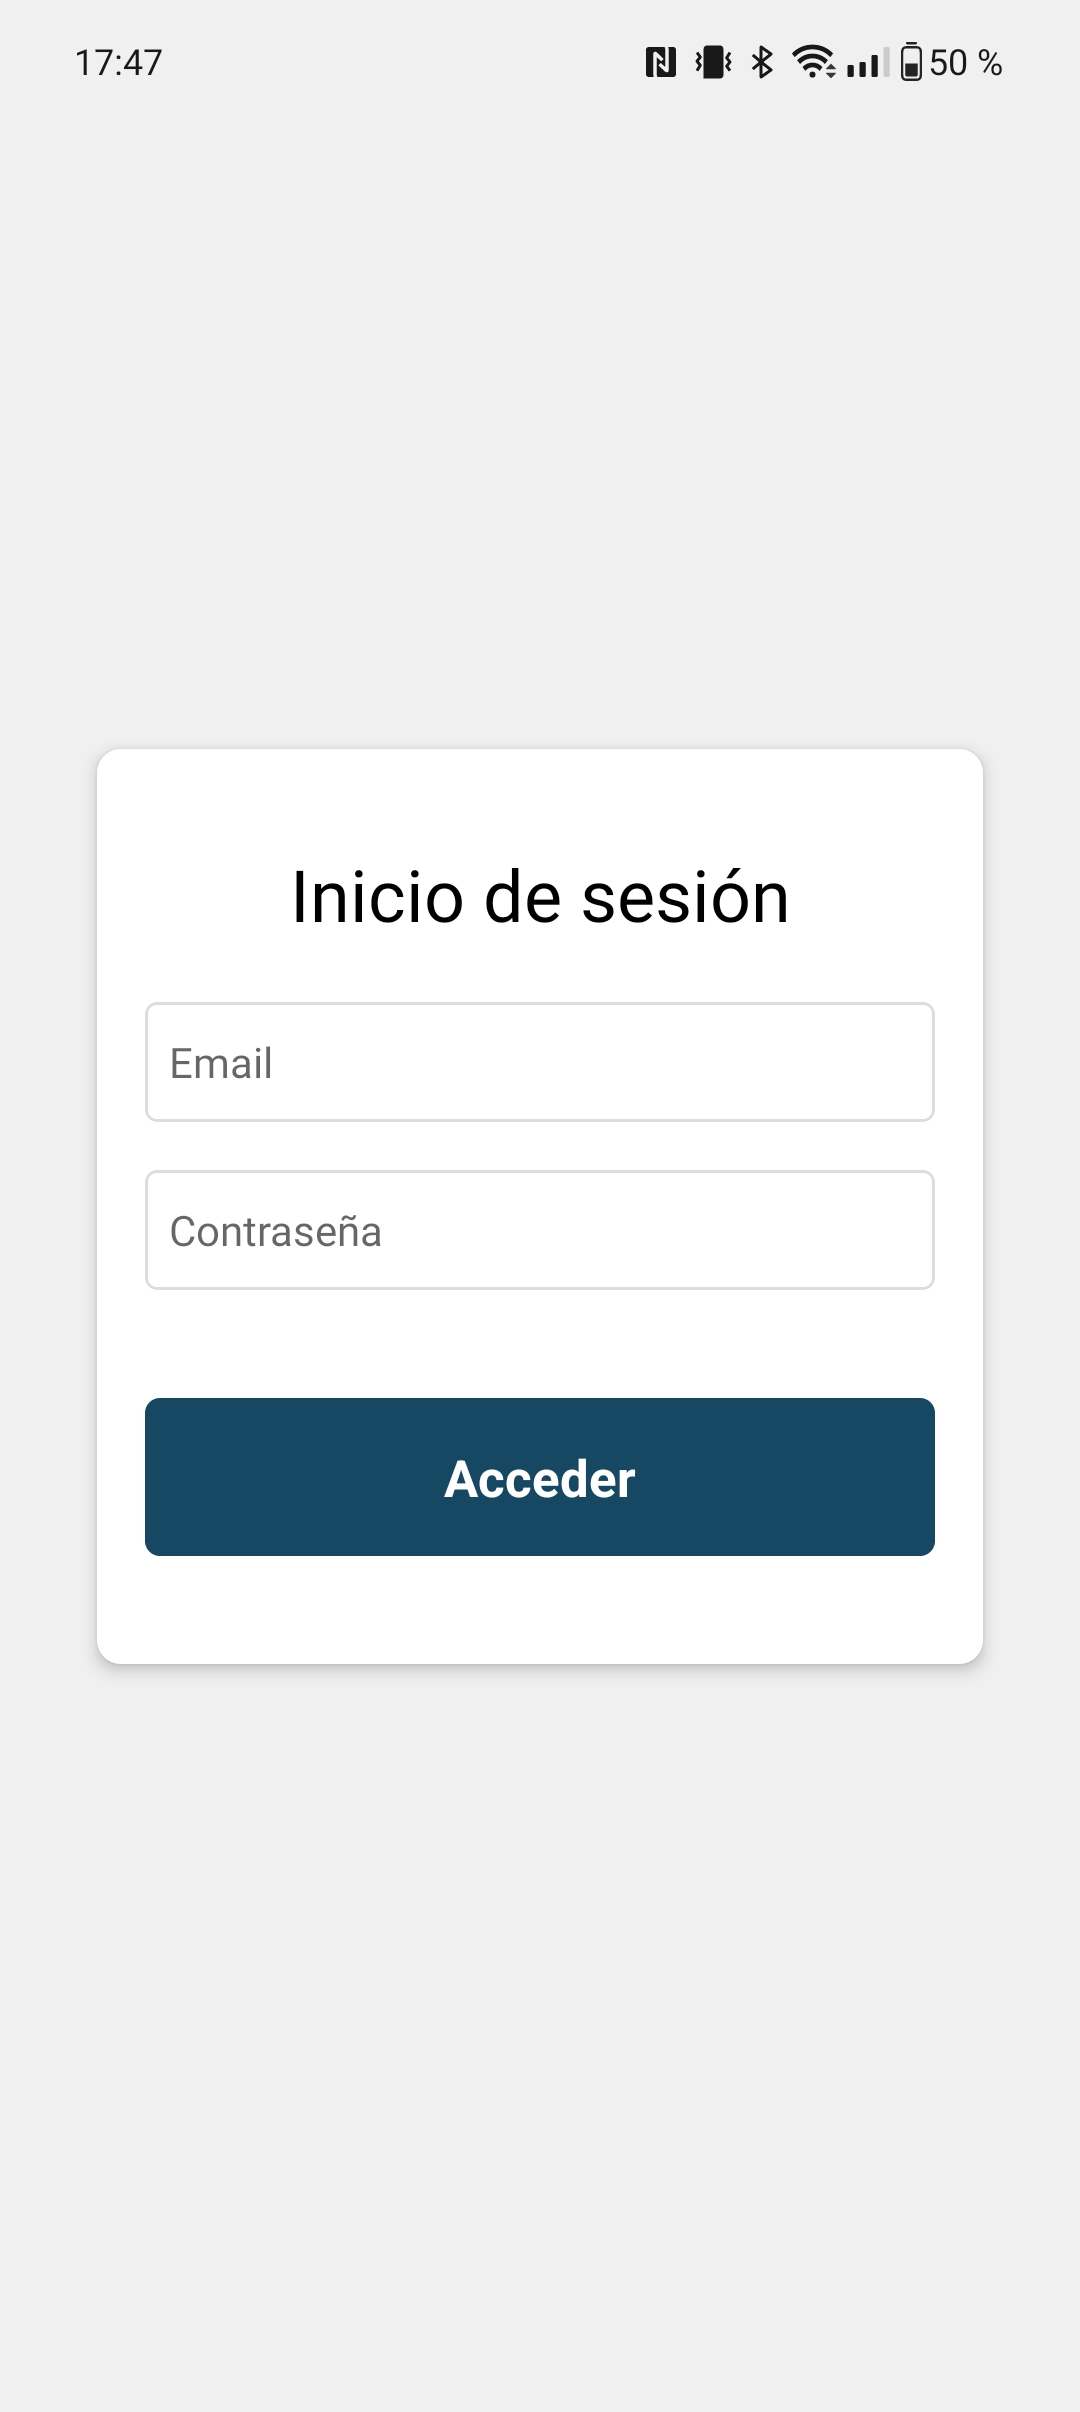
\includegraphics[width=0.40\textwidth]{inicioSesion}
	\caption[Pantalla inicio sesión]{Pantalla de inicio de sesión.}
	\label{fig:inicioSesion}
\end{figure}

\subsection{Pantalla inicio}

Tras una identificación exitosa, todos los usuarios serán redirigidos a la pantalla inicial (imagen \ref{fig:pantallaInicio}). Esta pantalla tiene los siguientes elementos:

\begin{itemize}

\item \textbf{Botón \textit{Crear Contrato}}: Al pulsar este botón se redigirá al usuario a una pantalla en la que mediante un formulario se podrá crear un contrato.

\item \textbf{Botón \textit{Firmar Contrato}}: Pulsando este botón se redirige al usuario a una pantalla donde aparecerán listados todos los contratos pendientes de firma que involucren al usuario.

\item \textbf{Botón \textit{Buscar Contratos}}: Este botón lleva al usuario a una pantalla donde puede buscar contratos que el empleador oferta dentro de la aplicación. 

\item \textbf{Botón \textit{Mis Contratos}}: Al pulsar este botón, el usuario es dirigido a una pantalla que lista todos los contratos en los que está involucrado, ya sea como dueño o como trabajador.
Los contratos pueden estar en distintos estados, bien activos o concluidos.

\end{itemize}

\begin{figure}[h]
	\centering
	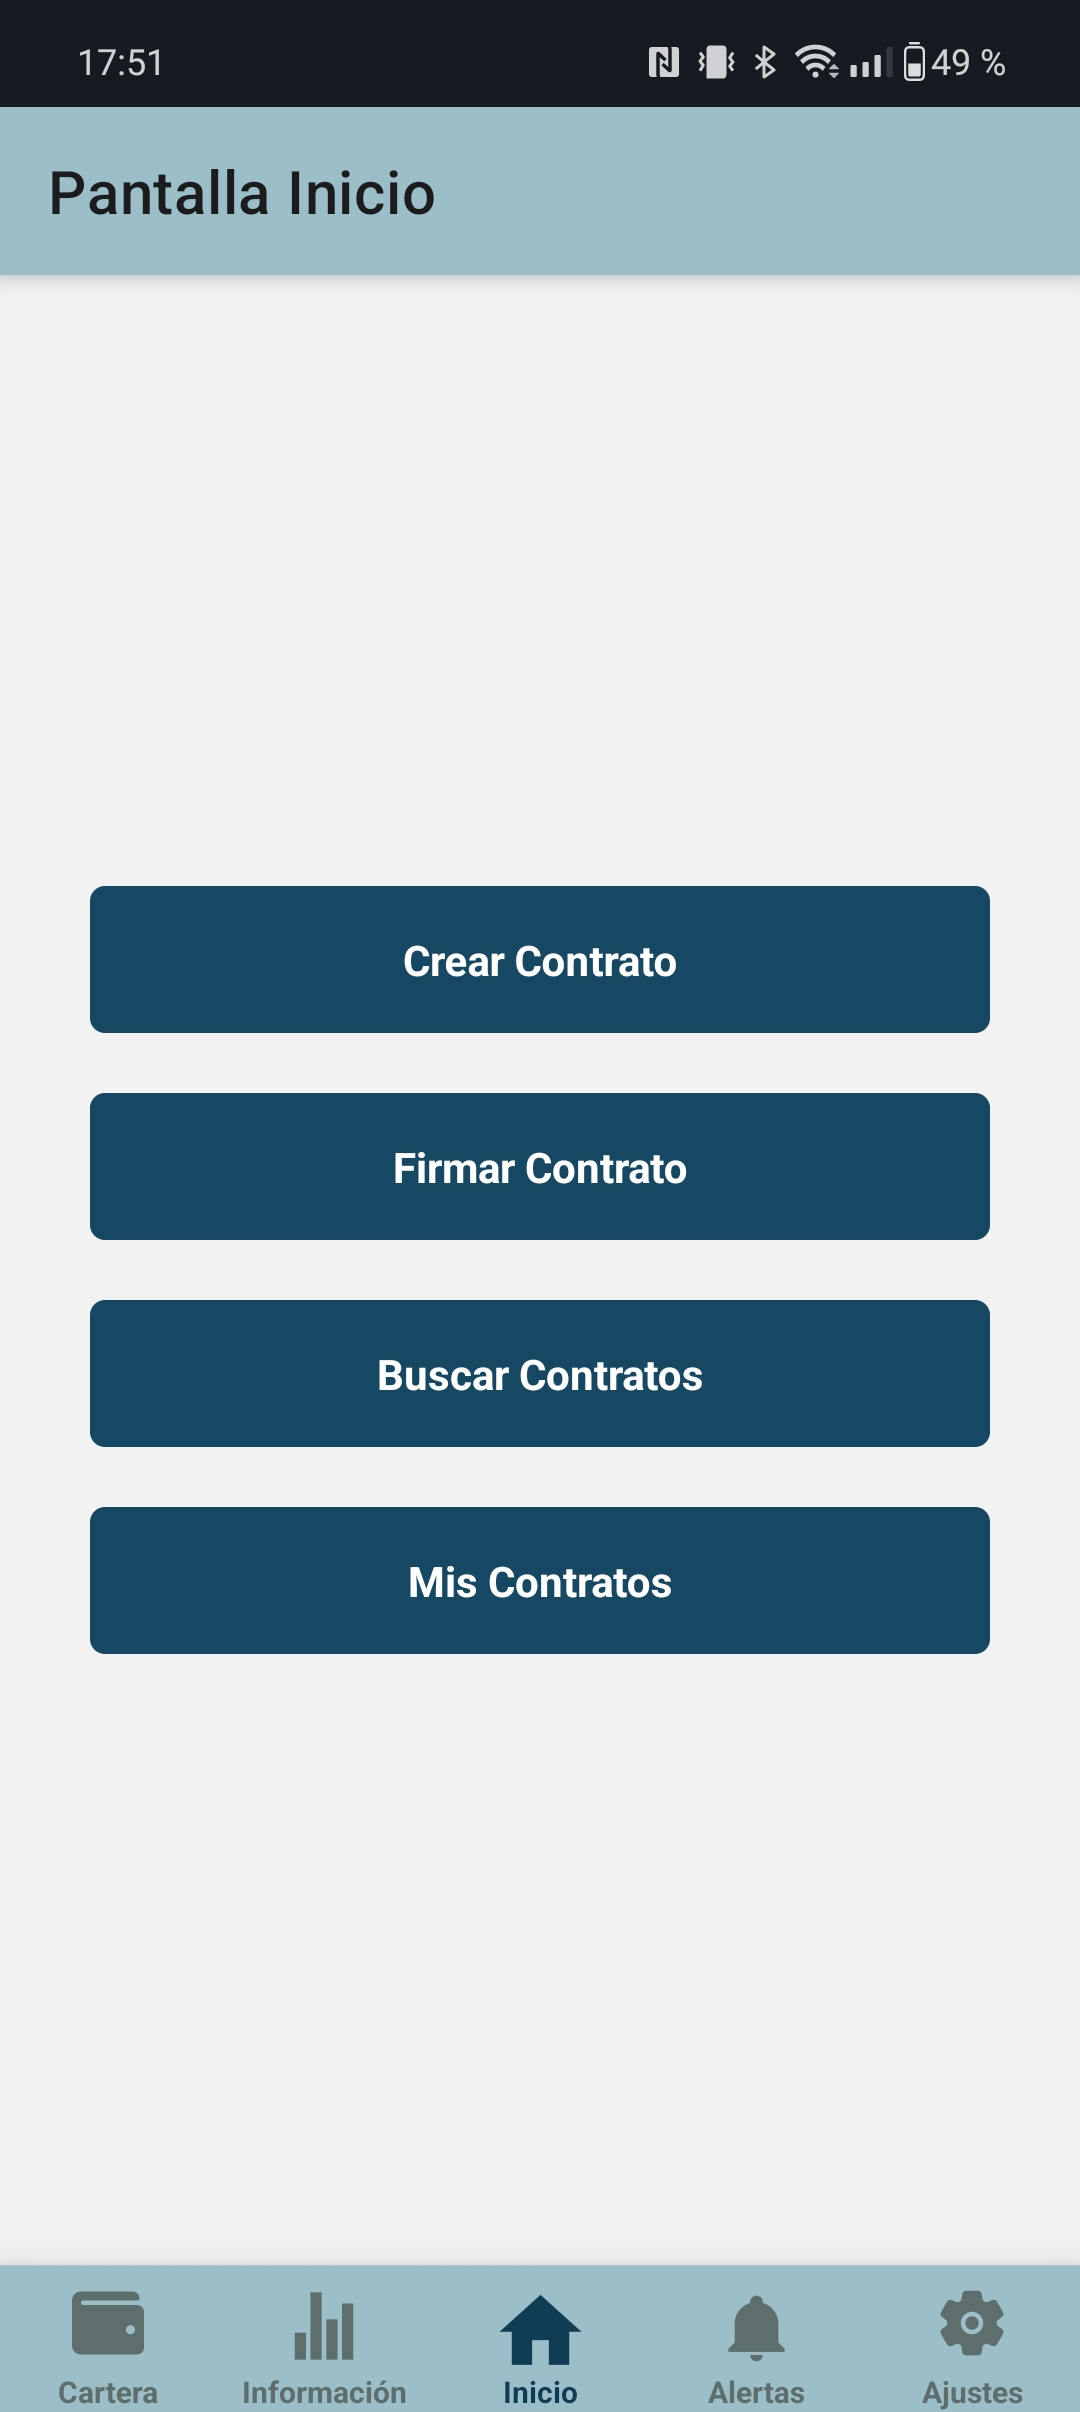
\includegraphics[width=0.40\textwidth]{pantallaInicio}
	\caption[Pantalla inicio]{Pantalla de inicio.}
	\label{fig:pantallaInicio}
\end{figure}


\subsection{Crear contrato}
\label{sec:CrearContrato}

Esta pantalla (ver imagen \ref{fig:crearContrato}) muestra una interfaz destinada a la creación de un contrato laboral, cuenta con los siguientes campos:

\begin{itemize}

\item \textbf{Título del contrato}: En este campo se debe ingresar el título del contrato.

\item \textbf{Descripción del contrato}: Aquí se especifican los detalles del contrato. Este campo es importante para definir claramente las tareas y expectativas de la posición.

\item \textbf{Dirección del destinatario}: Este campo está destinado para ingresar la dirección de la billetera del trabajador, la cual se usará tanto para identificar al trabajador como para ingresar el salario.
Cabe remarcar que este campo es opcional, y en el caso de no ser rellenado se considerará que se está ofertando el trabajo y se mostrará a todos los usuarios de la aplicación para su firma.

\item \textbf{Salario del trabajador}: En este campo se debe introducir el salario del trabajador, especificado en Ethereum.

\item \textbf{Fecha inicio y fin}: Estos campos se utilizan para definir la duración del contrato, indicando cuándo comenzará y terminará. Al introducir los datos aparecerá un calendario y un reloj permitiendo seleccionar la hora exacta de inicio y fin del contrato.

\end{itemize}

Finalmente, usando el botón `crear contrato', si todos los datos han sido introducidos correctamente, aparecerá una ventana emergente que confirmará que el contrato ha sido creado.
En caso de querer retroceder, el usuario puede usar el botón de retroceso del móvil o cualquiera de los botones del menú de la aplicación.

\begin{figure}[h]
	\centering
	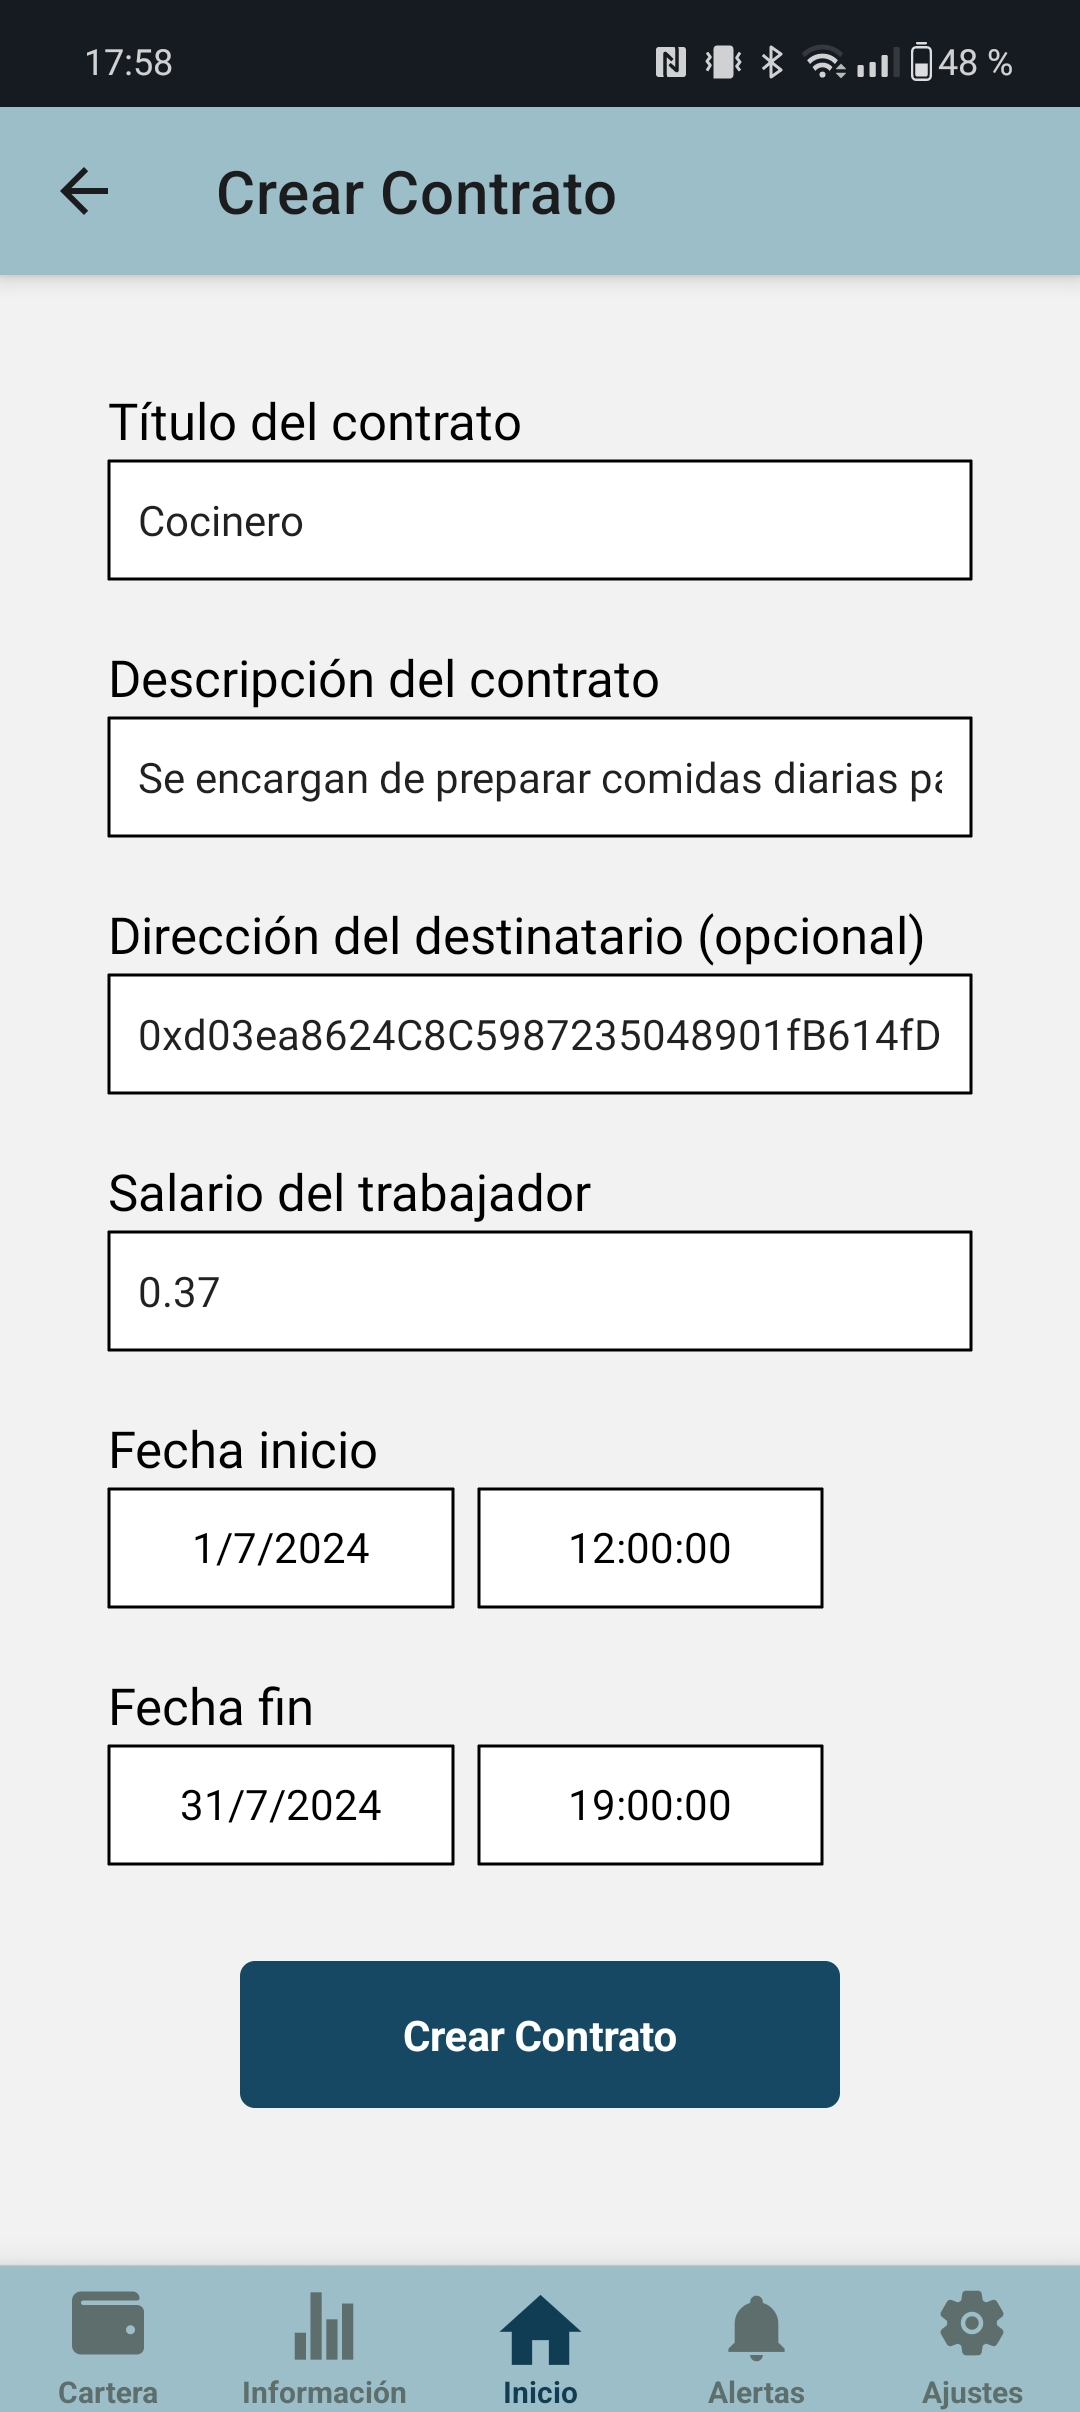
\includegraphics[width=0.40\textwidth]{crearContrato}
	\caption[Pantalla crear contrato]{Pantalla crear contrato.}
	\label{fig:crearContrato}
\end{figure}


\subsection{Firmar contrato}

La pantalla `Firmar contrato' (imagen \ref{fig:firmarContrato}) está diseñada para gestionar la firma de contratos pendientes.
En esta pantalla aparece una lista con los contratos que involucren a un trabajador y todavía no hayan sido firmados.
Al tocar sobre el contrato listado, se redirige al usuario a una nueva pantalla donde se presentan los detalles completos del contrato y finalmente un botón que permite firmar un contrato usando la huella digital o reconocimiento facial.
Por otro lado, también se posibilita al usuario a firmar un contrato mediante un código QR asociado a un contrato específico. Para ello en la parte superior derecha existe un enlace que abre la cámara del dispositivo.
Este método agiliza el proceso de firma asegurando la identificación del usuario.

\begin{figure}[h]
	\centering
	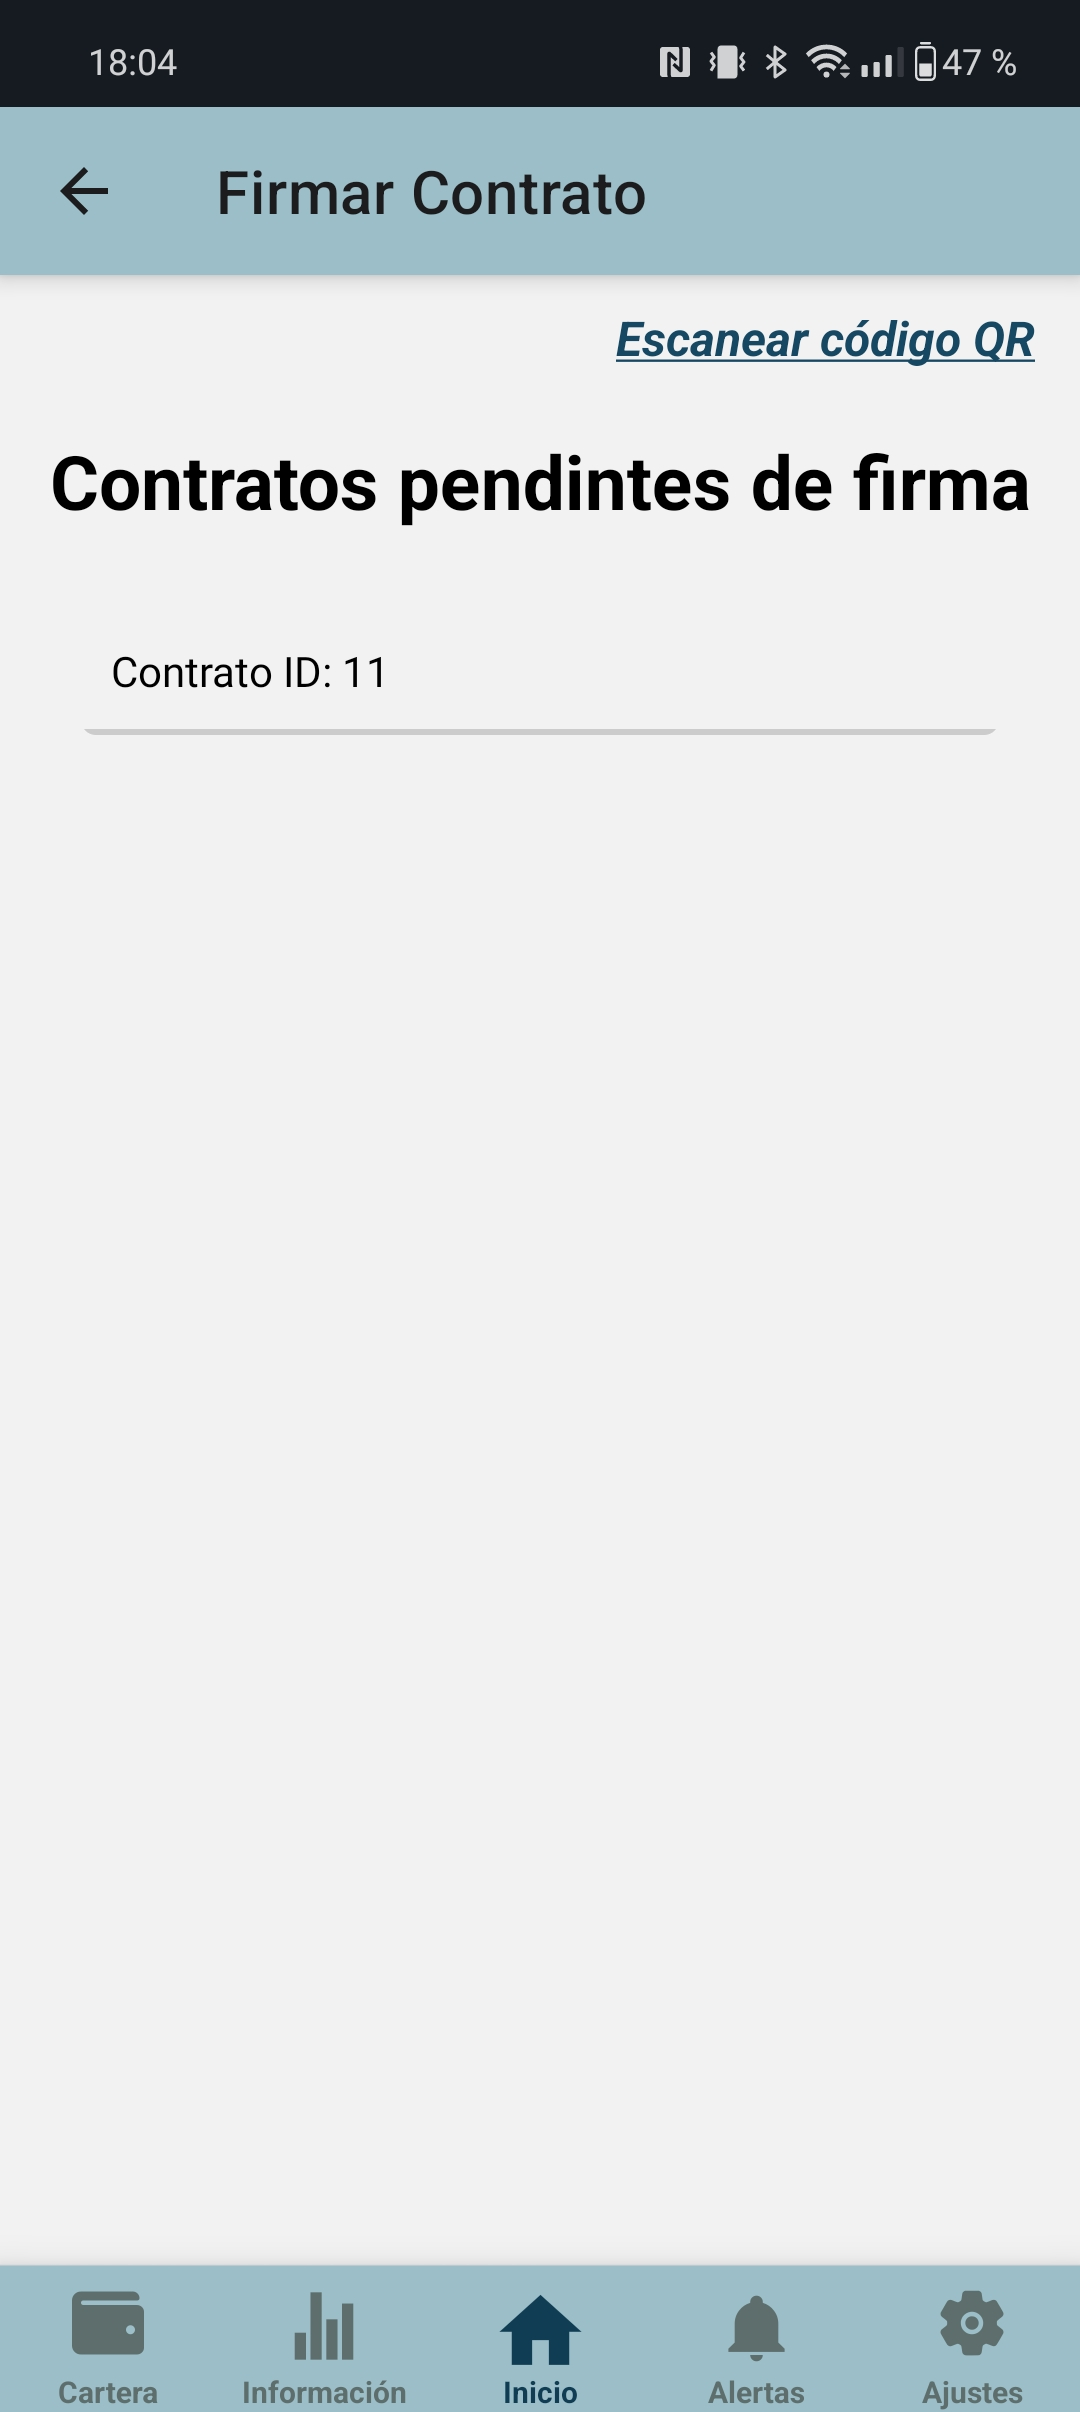
\includegraphics[width=0.40\textwidth]{firmarContrato}
	\caption[Pantalla firmar contrato]{Pantalla firmar contrato.}
	\label{fig:firmarContrato}
\end{figure}


\subsection{Buscar contratos}

Esta pantalla actúa como un tablón de ofertas de trabajo, donde los contratos que aún no tienen asignado un trabajador están listados para que los usuarios puedan explorar y seleccionar oportunidades de empleo según sus intereses y habilidades. 
Este diseño permite a los usuarios tener una visión rápida de las condiciones laborales y la duración de cada contrato. Ver imagen \ref{fig:buscarContratos}

En el caso de estar interesado, al seleccionar un contrato específico de la lista, el usuario será dirigido a otra pantalla donde puede ver detalles más extensos del contrato. Desde esta pantalla de información, el usuario tiene la opción de firmar el contrato, facilitando así la conexión entre empleadores y potenciales trabajadores.

\begin{figure}[h]
	\centering
	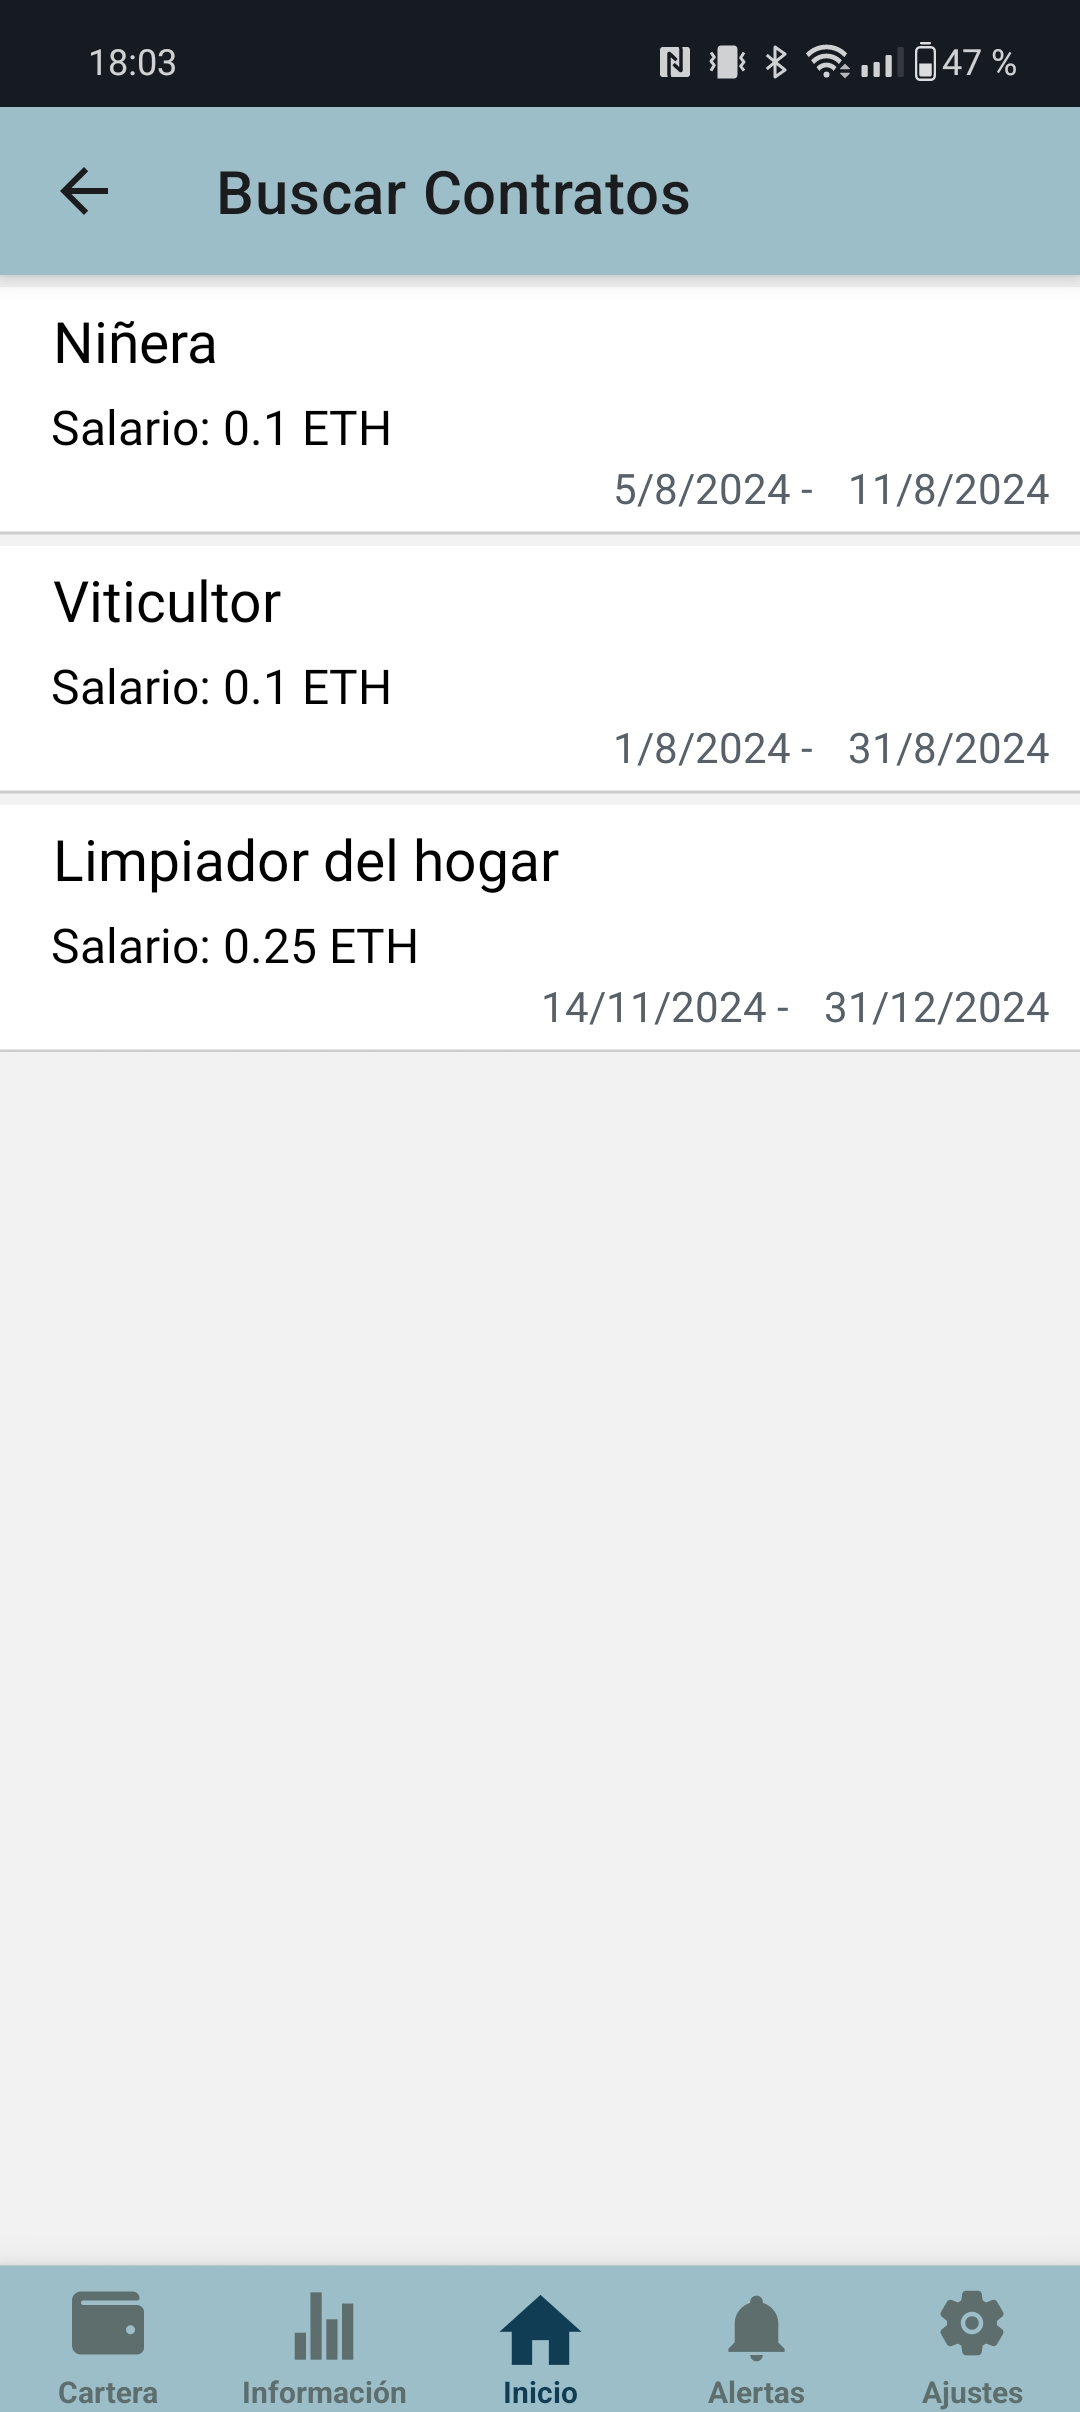
\includegraphics[width=0.40\textwidth]{buscarContratos}
	\caption[Pantalla buscar contratos]{Pantalla buscar contratos.}
	\label{fig:buscarContratos}
\end{figure}



\subsection{Mis contratos}

Esta pantalla (ver imagen \ref{fig:misContratos}) esta diseñada para permitir a los usuarios gestionar y revisar los contratos en los que están involucrados, ya sea como empleador o como trabajador.
La pantalla incluye dos secciones principales, las cuales han sido etiquetadas como `contratos como empleador' y `contratos como trabajador'. Los usuarios pueden pinchar las etiquetas ubicadas en la parte superior para alternar de una sección a otra, o simplemente deslizar el dedo hacía la derecha o la izquierda.

En la primera sección se muestran todos los contratos iniciados en los que el usuario figura como empleador. En la parte superior aparecerán los contratos que se encuentren activos, mientras que pulsando el botón inferior `Mostrar Contratos Finalizados' se abrirá un desplegable el cual nos permitirá consultar todos los contratos que han expirado.

Por otro lado, en la segunda sección, se muestran los contratos iniciados en los que el usuario figura como trabajador. Del mismo modo que en el caso anterior, en la parte superior aparecerán los contratos que todavía no han finalizado, mientras que en el desplegable inferior se podrán consultar los contratos finalizados.

Al seleccionar cualquier contrato de la lista, el usuario pude acceder a los detalles del mismo y dependiendo del rol que tenga el usuario, tendrá la opción de finalizar el contrato, liberar el salario, realizar una modificación o simplemente consular el contrato.

Esta pantalla está diseñada para ser sencilla y funcional, pudiendo mostrar una gran cantidad de información lo más ordenada y visual posible.

\begin{figure}[h]
	\label{fig:misContratos}
	\centering
	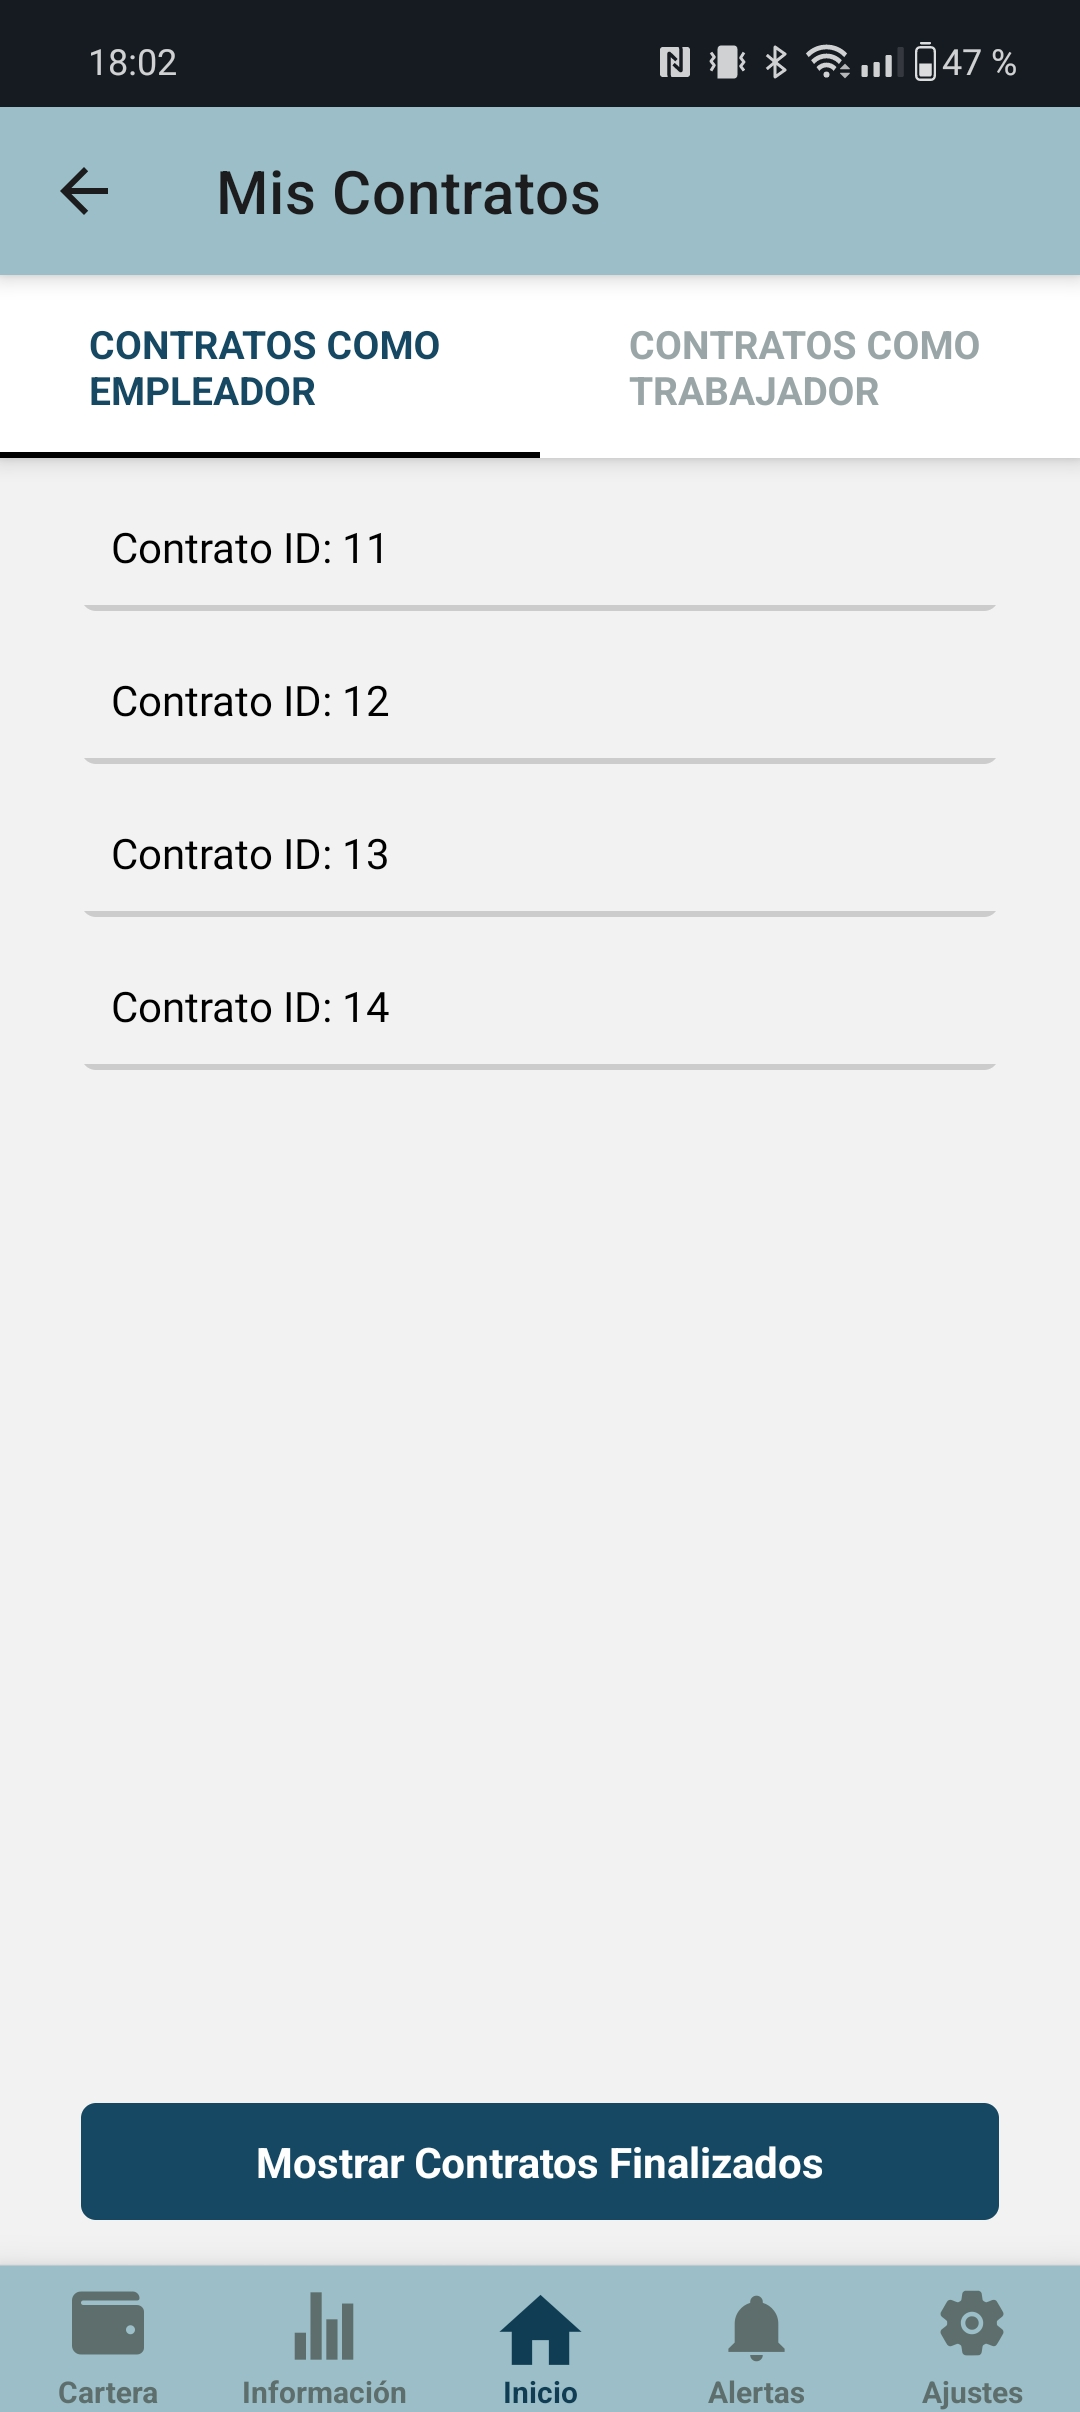
\includegraphics[width=0.40\textwidth]{misContratos}
	\caption[Pantalla contratos del usuario]{Pantalla que muestra los contratos del usuario.}
	\label{fig:misContratos}
\end{figure}


\subsection{Detalles contrato}

La pantalla `Consultar Contratos' esta diseñada para permitir a los usuarios consultar todos los detalles de un contrato específico.

Como se puede ver en la imagen \ref{fig:infoContrato}, esta pantalla muestra todos los campos explicados previamente en la sección de creación de un contrato. Sin embargo, incluye dos campos adicionales: uno que muestra la billetera del empleador, identificándolo en el proceso, y otro que muestra el estado del contrato. El estado puede ser `pendiente' si el contrato todavía no se ha firmado, `activo' si el contrato se encuentra dentro de las fechas acordadas, `finalizado' si ha superado la fecha de expiración, o `pausado' si se ha decidido pausar el contrato tras una modificación.

Es importante destacar que la imagen presentada en este apartado se ha tomado desde una \textit{tablet} en lugar de un teléfono móvil. Esto se hace con el propósito de demostrar cómo la aplicación se adapta a dispositivos de diferentes tamaños. En el caso de la \textit{tablet}, toda la información se muestra en una sola pantalla sin necesidad de desplazarse. En cambio, en un dispositivo móvil, sería necesario deslizar hacia arriba o hacia abajo para visualizar toda la información.

\begin{figure}[h]
	\centering
	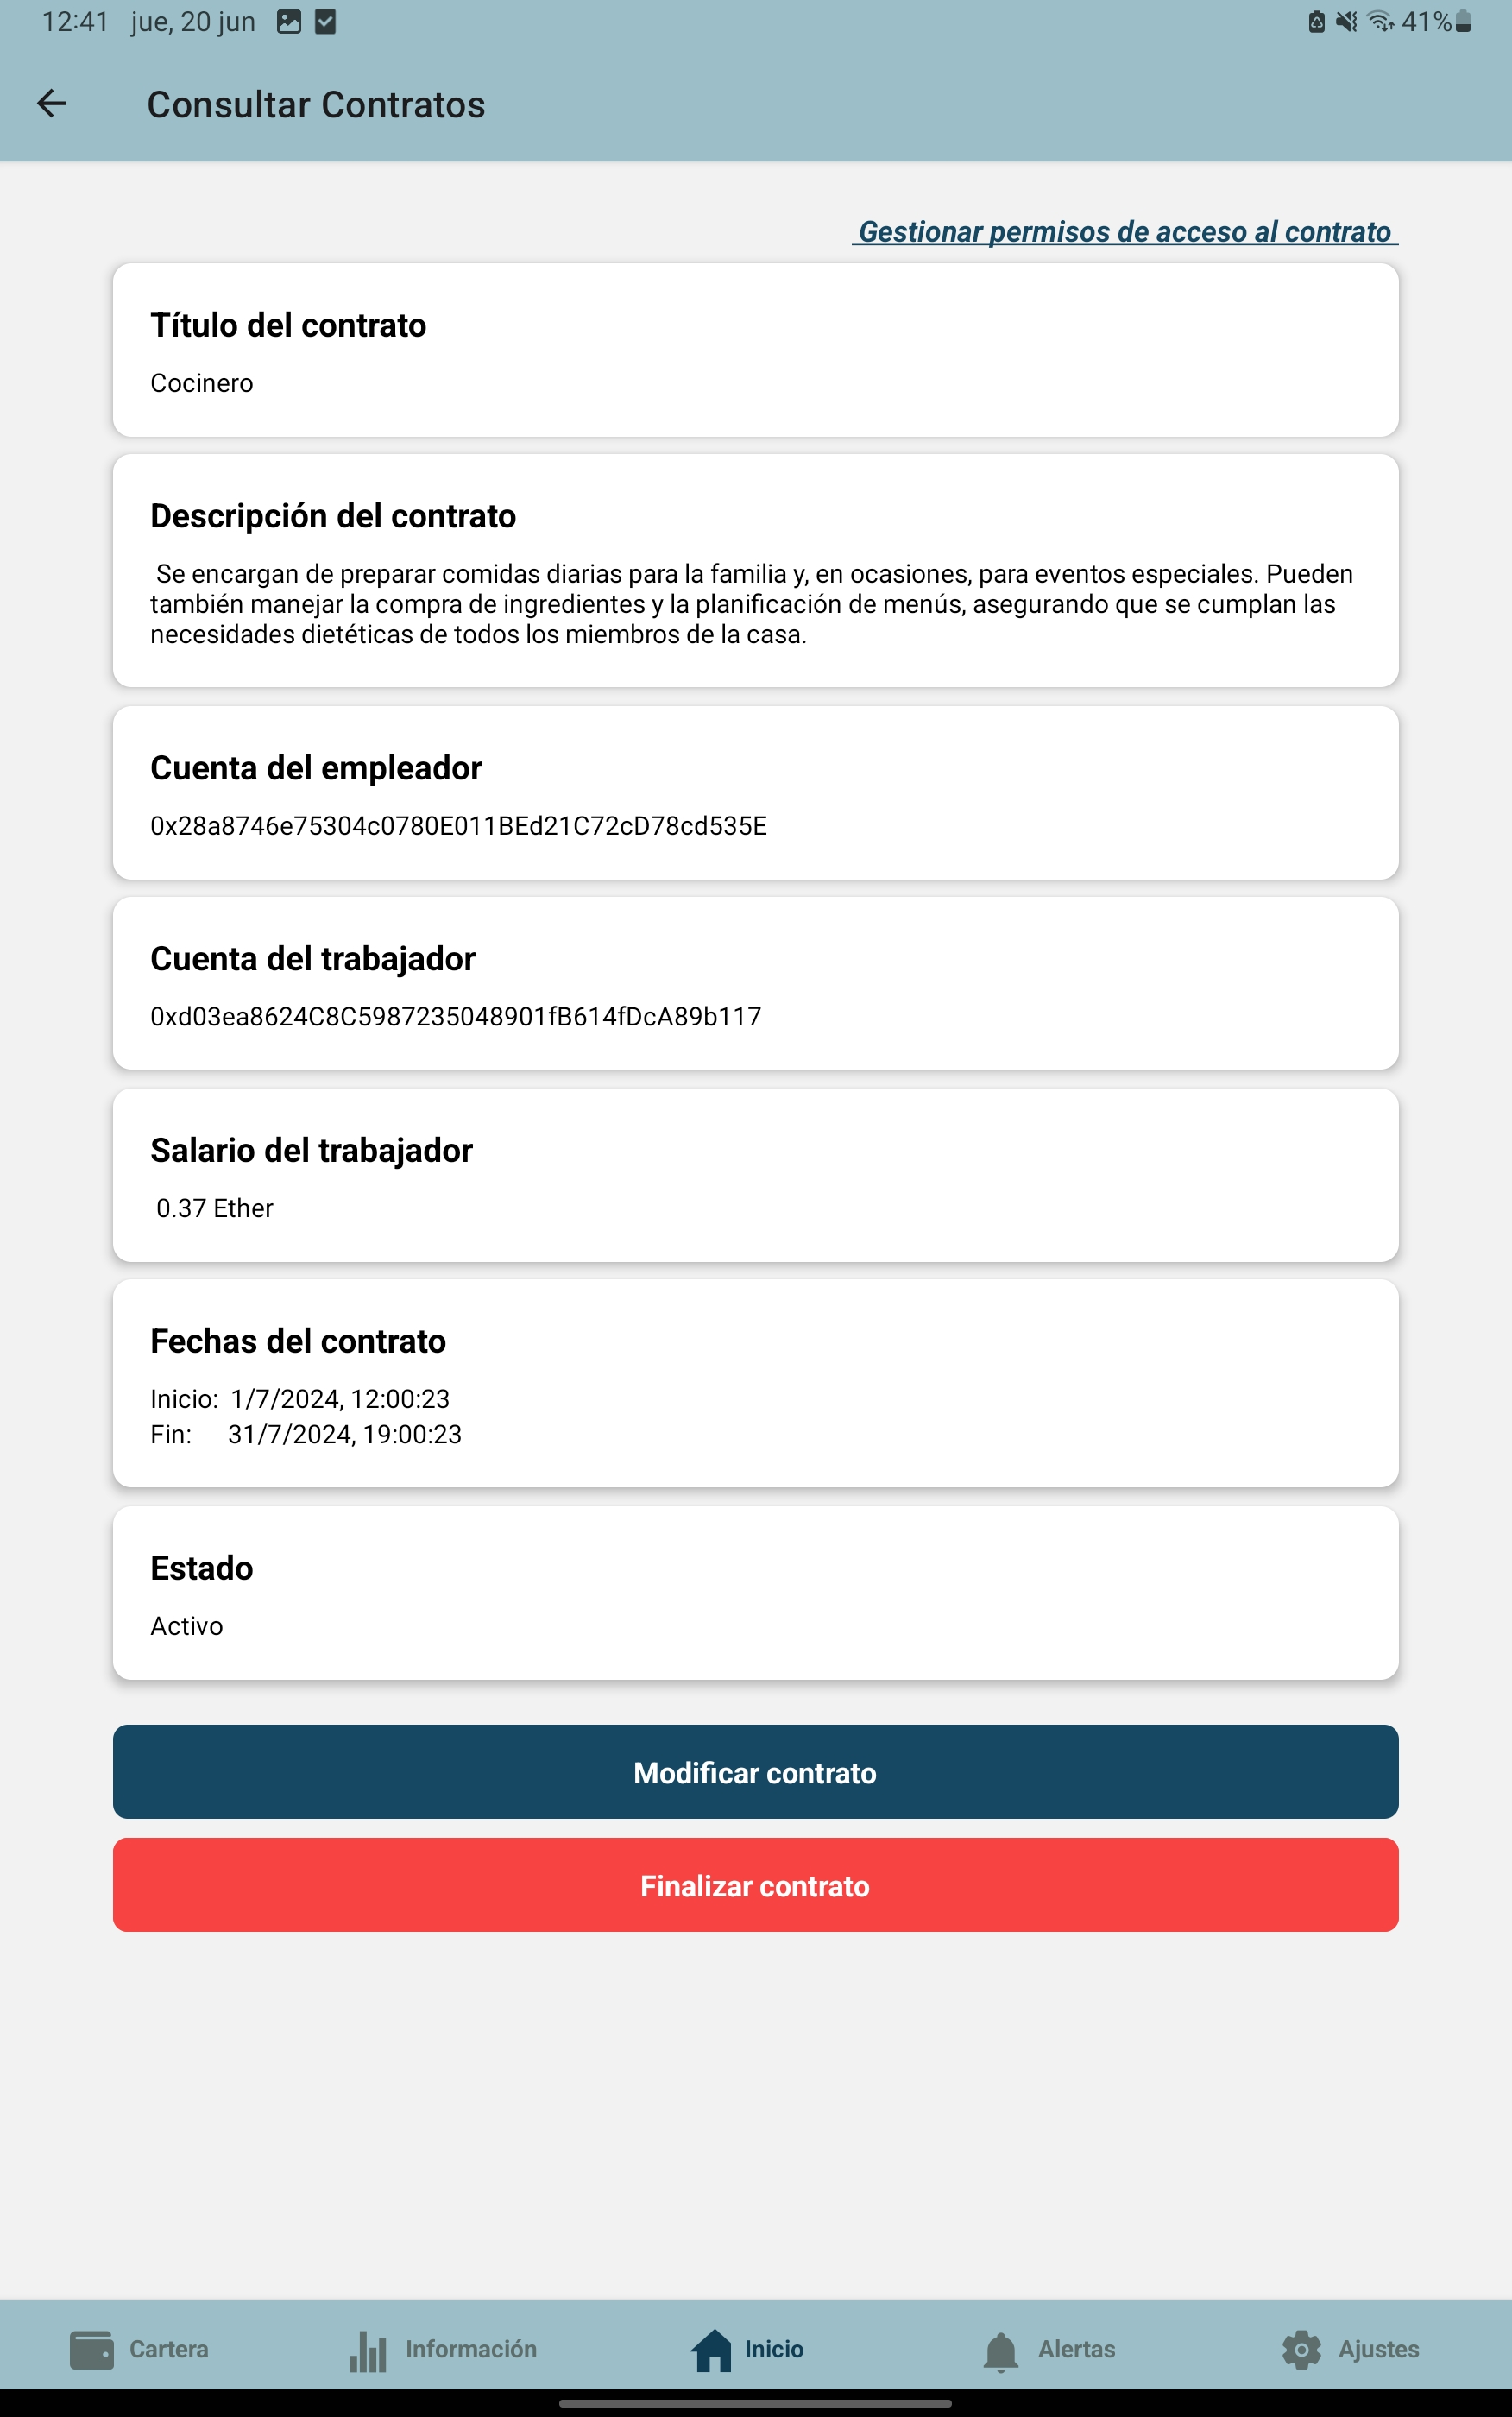
\includegraphics[width=0.50\textwidth]{infoContrato}
	\caption[Pantalla detalles del contrato]{Pantalla que muestra los detalles del contrato.}
	\label{fig:infoContrato}
\end{figure}

Esta pantalla recoge una gran variedad de funcionalidades, que se mostrarán al usuario dependiendo de su rol en el contrato y del estado actual del mismo.
Para los usuarios que desempeñan el papel de empleadores dentro del contrato, se ofrecen las siguientes opciones:

\begin{itemize}
\item \textbf{Gestión de permisos}: Permite al empleador gestionar y controlar quién puede ver y modificar detalles del contrato.

\item \textbf{Cancelar contrato}: Esta opción solo se encuentra disponible cuando el contrato no ha sido firmado, dando la posibilidad al usuario de cancelar el contrato y recuperar el dinero depositado en el mismo.

\item \textbf{Modificar contrato}: Facilita la actualización de los términos del contrato cuando este se encuentre activo. Se enviará una propuesta con los cambios sugeridos que tendrá que ser aprobada por el trabajador.

\item \textbf{Finalizar contrato}: Permite al empleador cerrar formalmente el contrato antes de su fecha de expiración si se considera que todas las obligaciones han sido cumplidas, marcando el final del compromiso laboral.

\item \textbf{Liberar pago}: Cuando el contrato se encuentre finalizado, se habilita esta opción para que el empleador pueda liberar el pago del salario al trabajador.
\end{itemize}

Por otro lado, desde la perspectiva del trabajador, además de poder consultar los detalles completos del contrato, dispondrá de la funcionalidad exclusiva de revisar cualquier propuesta de modificación del contrato. Esta opción se activa solo cuando existen cambios pendientes de revisión, permitiendo al usuario acceder a una pantalla donde evaluar los cambios y responder a la modificación sugerida.


\subsection{Modificar Contrato y aprobar cambios}

En este apartado se presentan dos funciones interrelacionadas. La primera es la modificación de un contrato, como se ilustra en la primera pantalla de la imagen \ref{fig:modificarCambios}. 
Una vez el contrato se encuentre firmado, el empleador tiene la posibilidad de proponer modificación a los términos del contrato existente. 

Los aspectos a modificar recogen:
\begin{itemize}

\item \textbf{Título}: Actualización del título del contrato.

\item \textbf{Descripción}: Ajuste de los detalles del contrato.

\item \textbf{Salario}: modificación de la cantidad del salario: si se incrementa, será necesario depositar la nueva cantidad al contrato, mientras que si se decrementa, la diferencia será devuelta al empleador. 

\item \textbf{Duración}: Permite modificar la fecha de finalización del contrato.

\item \textbf{Pausa del contrato}: Posibilidad de pausar temporalmente el contrato. Al reactivarse, se añadirá al contrato el tiempo que estuvo pausado.

\end{itemize}

Tras enviar la propuesta de modificación, el trabajador recibirá una alerta que le notificará que hay cambios propuestos. Al acceder a la segunda pantalla de la imagen \ref{fig:modificarCambios}, se puede observar en verde los detalles modificados respecto a los términos originales. Después de revisar estos cambios, el trabajador tendrá la opción de aceptar o rechazar los cambios propuestos, asegurando así su acuerdo antes de que los cambios se efectúen.

\begin{figure}[h]
	\centering
	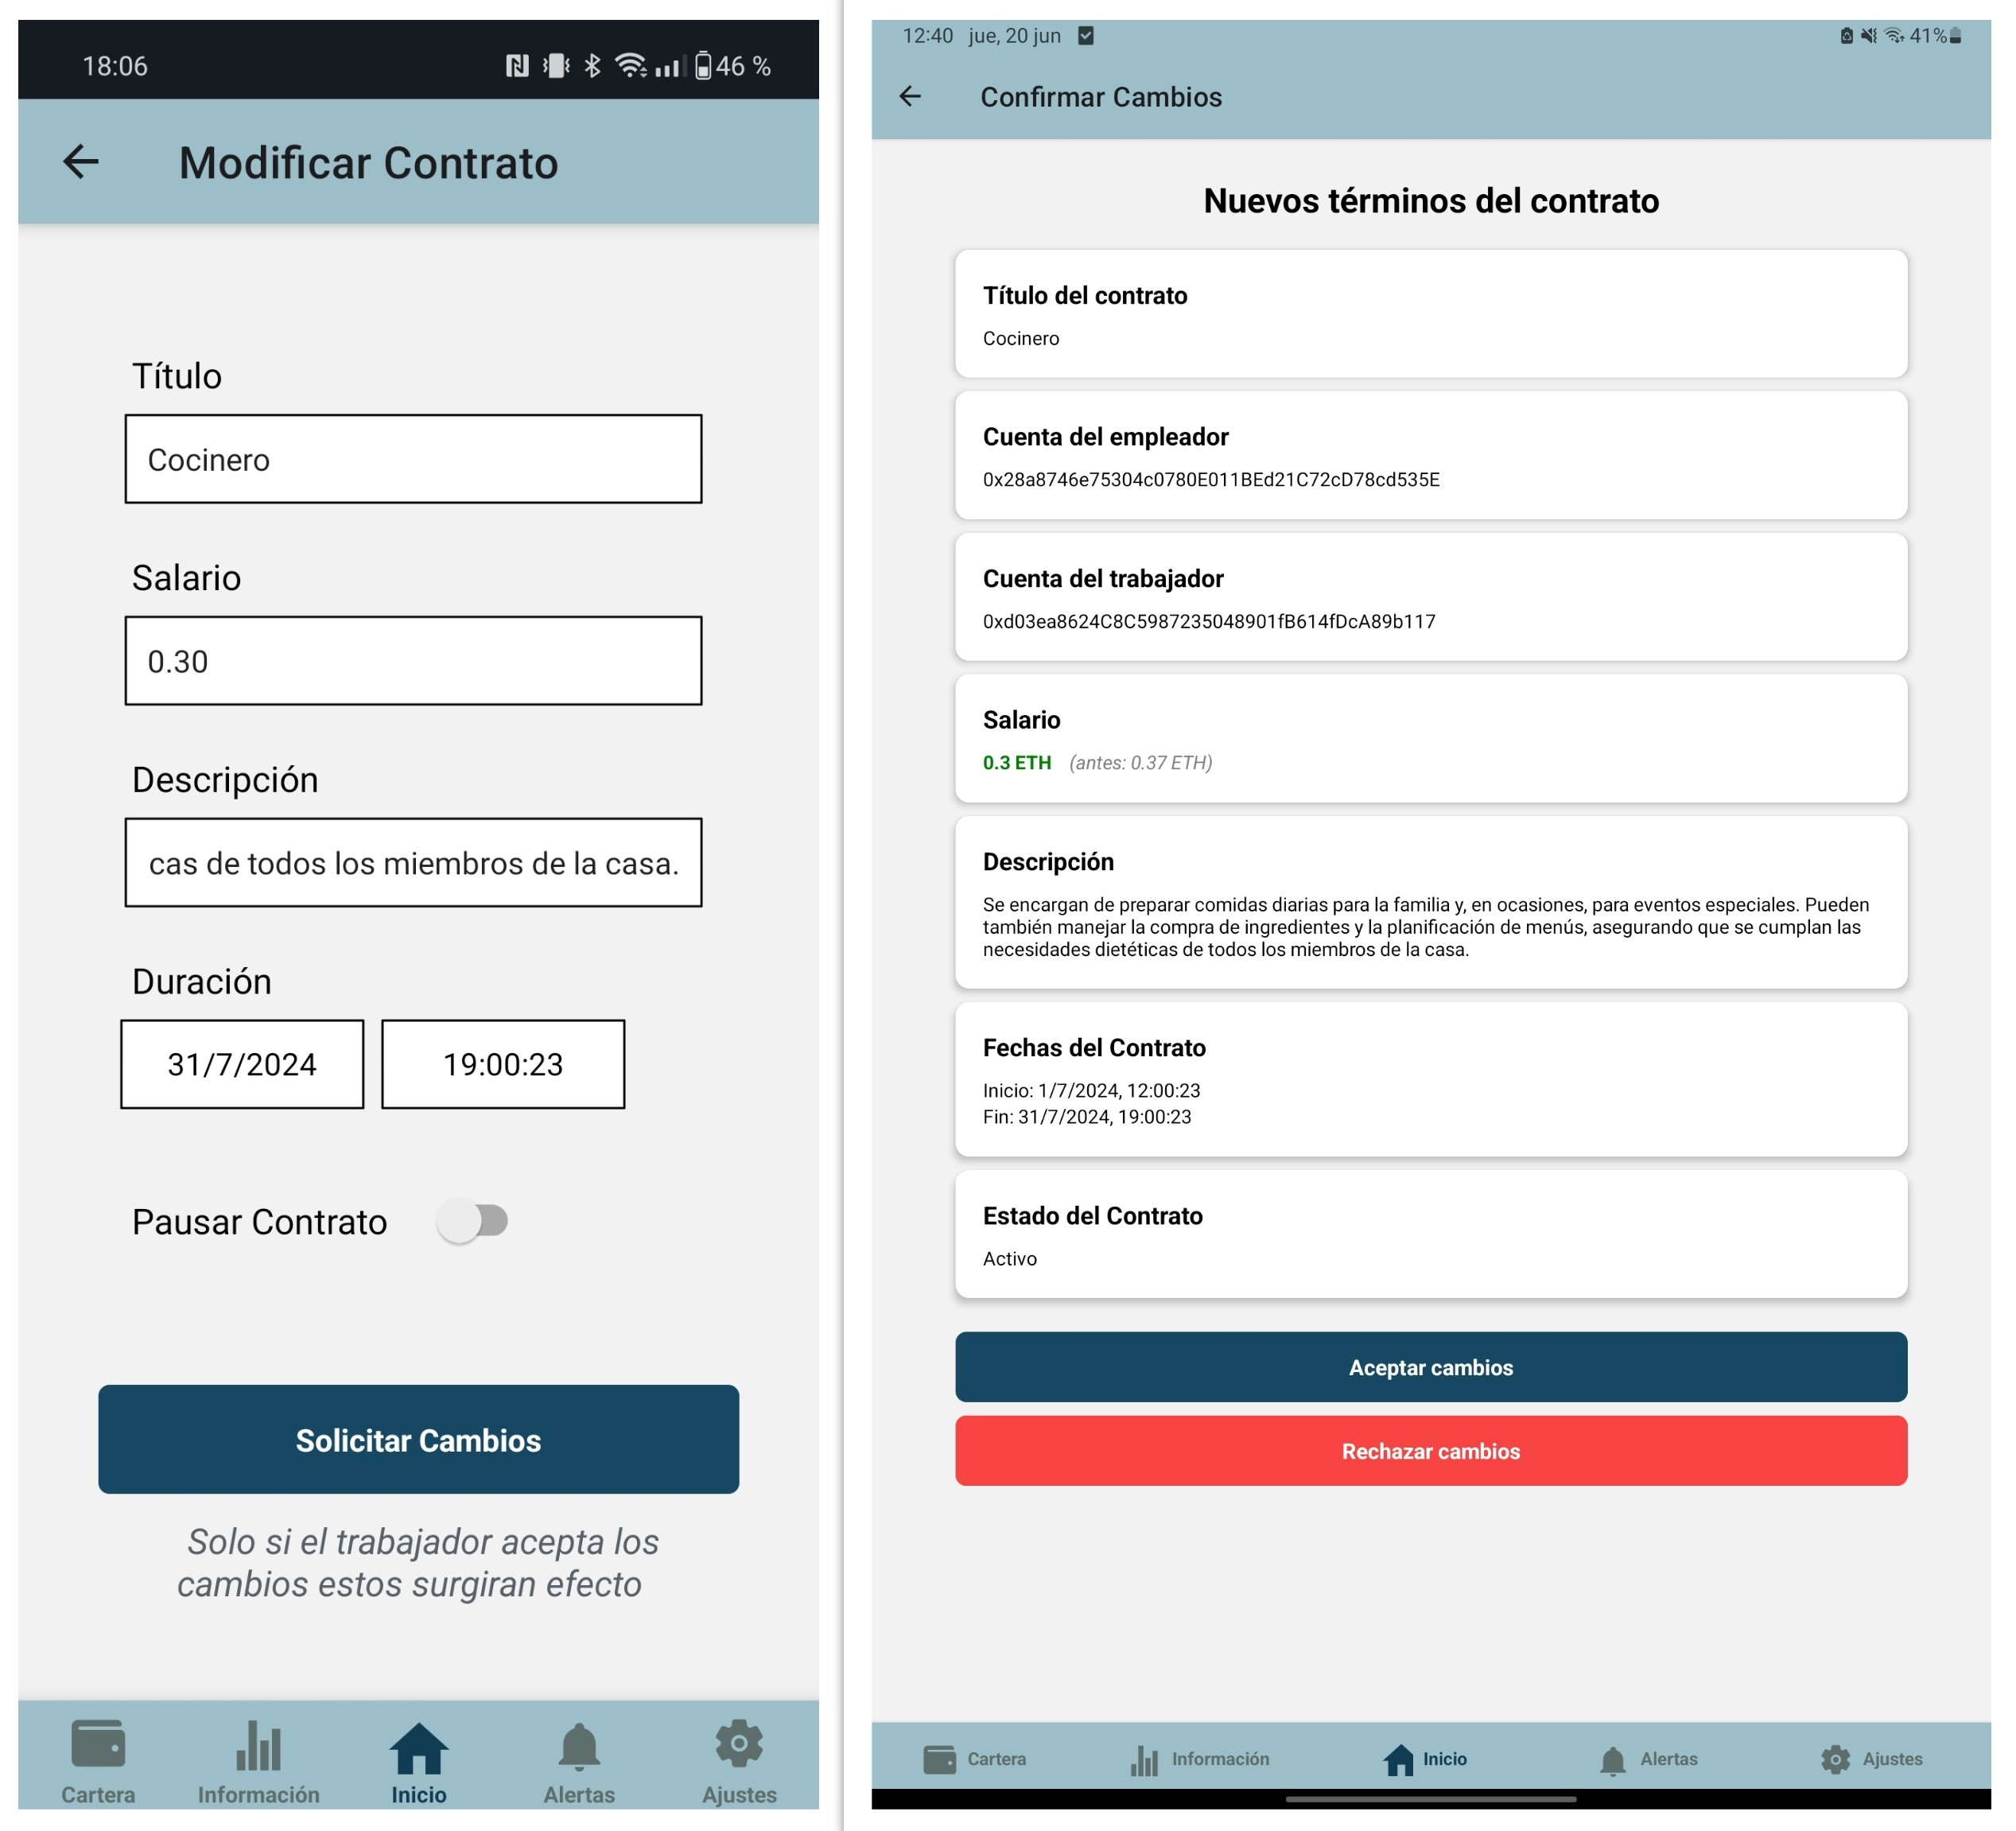
\includegraphics[width=0.90\textwidth]{modificarCambios}
	\caption[Pantalla modificar contrato]{Pantallas de propuesta de modificación y aprobación de cambios.}
	\label{fig:modificarCambios}
\end{figure}


\subsection{Añadir mánager y código QR}

Como mencionó en apartados anteriores, dos de las funcionalidades destacadas en la pantalla de detalles del contrato incluyen la adición de un tercero para su gestión y la visualización del código QR para la firma del contrato.

La primera pantalla, ver imagen \ref{fig:managerQR}, está diseñada para otorgar permisos de visualización y gestión sobre un contrato a un usuario designado.
Para ello, el empleador introduce la dirección de la billetera del usuario deseado, y luego lo asigna pulsando el botón `Asignar Manager'.
Una vez asignado, el nuevo mánager se añade a una lista de \textit{managers} actualmente asignados. Desde esta lista, del mismo modo se pude borrar un mánager pulsando un emoticono que representa una papelera.

La segunda pantalla de la imagen \ref{fig:managerQR}, se visualiza al presionar el botón `Mostrar Código QR' desde la pantalla \ref{fig:infoContrato}.
Esta opción está disponible únicamente cuando el contrato aún no ha sido firmado. Al activar esta función, se genera un código QR, como se observa en la pantalla. La descripción bajo el código explica que, al escanear este código QR, el contrato será automáticamente firmado por el usuario que realiza el escaneo.

\begin{figure}[h]
	\centering
	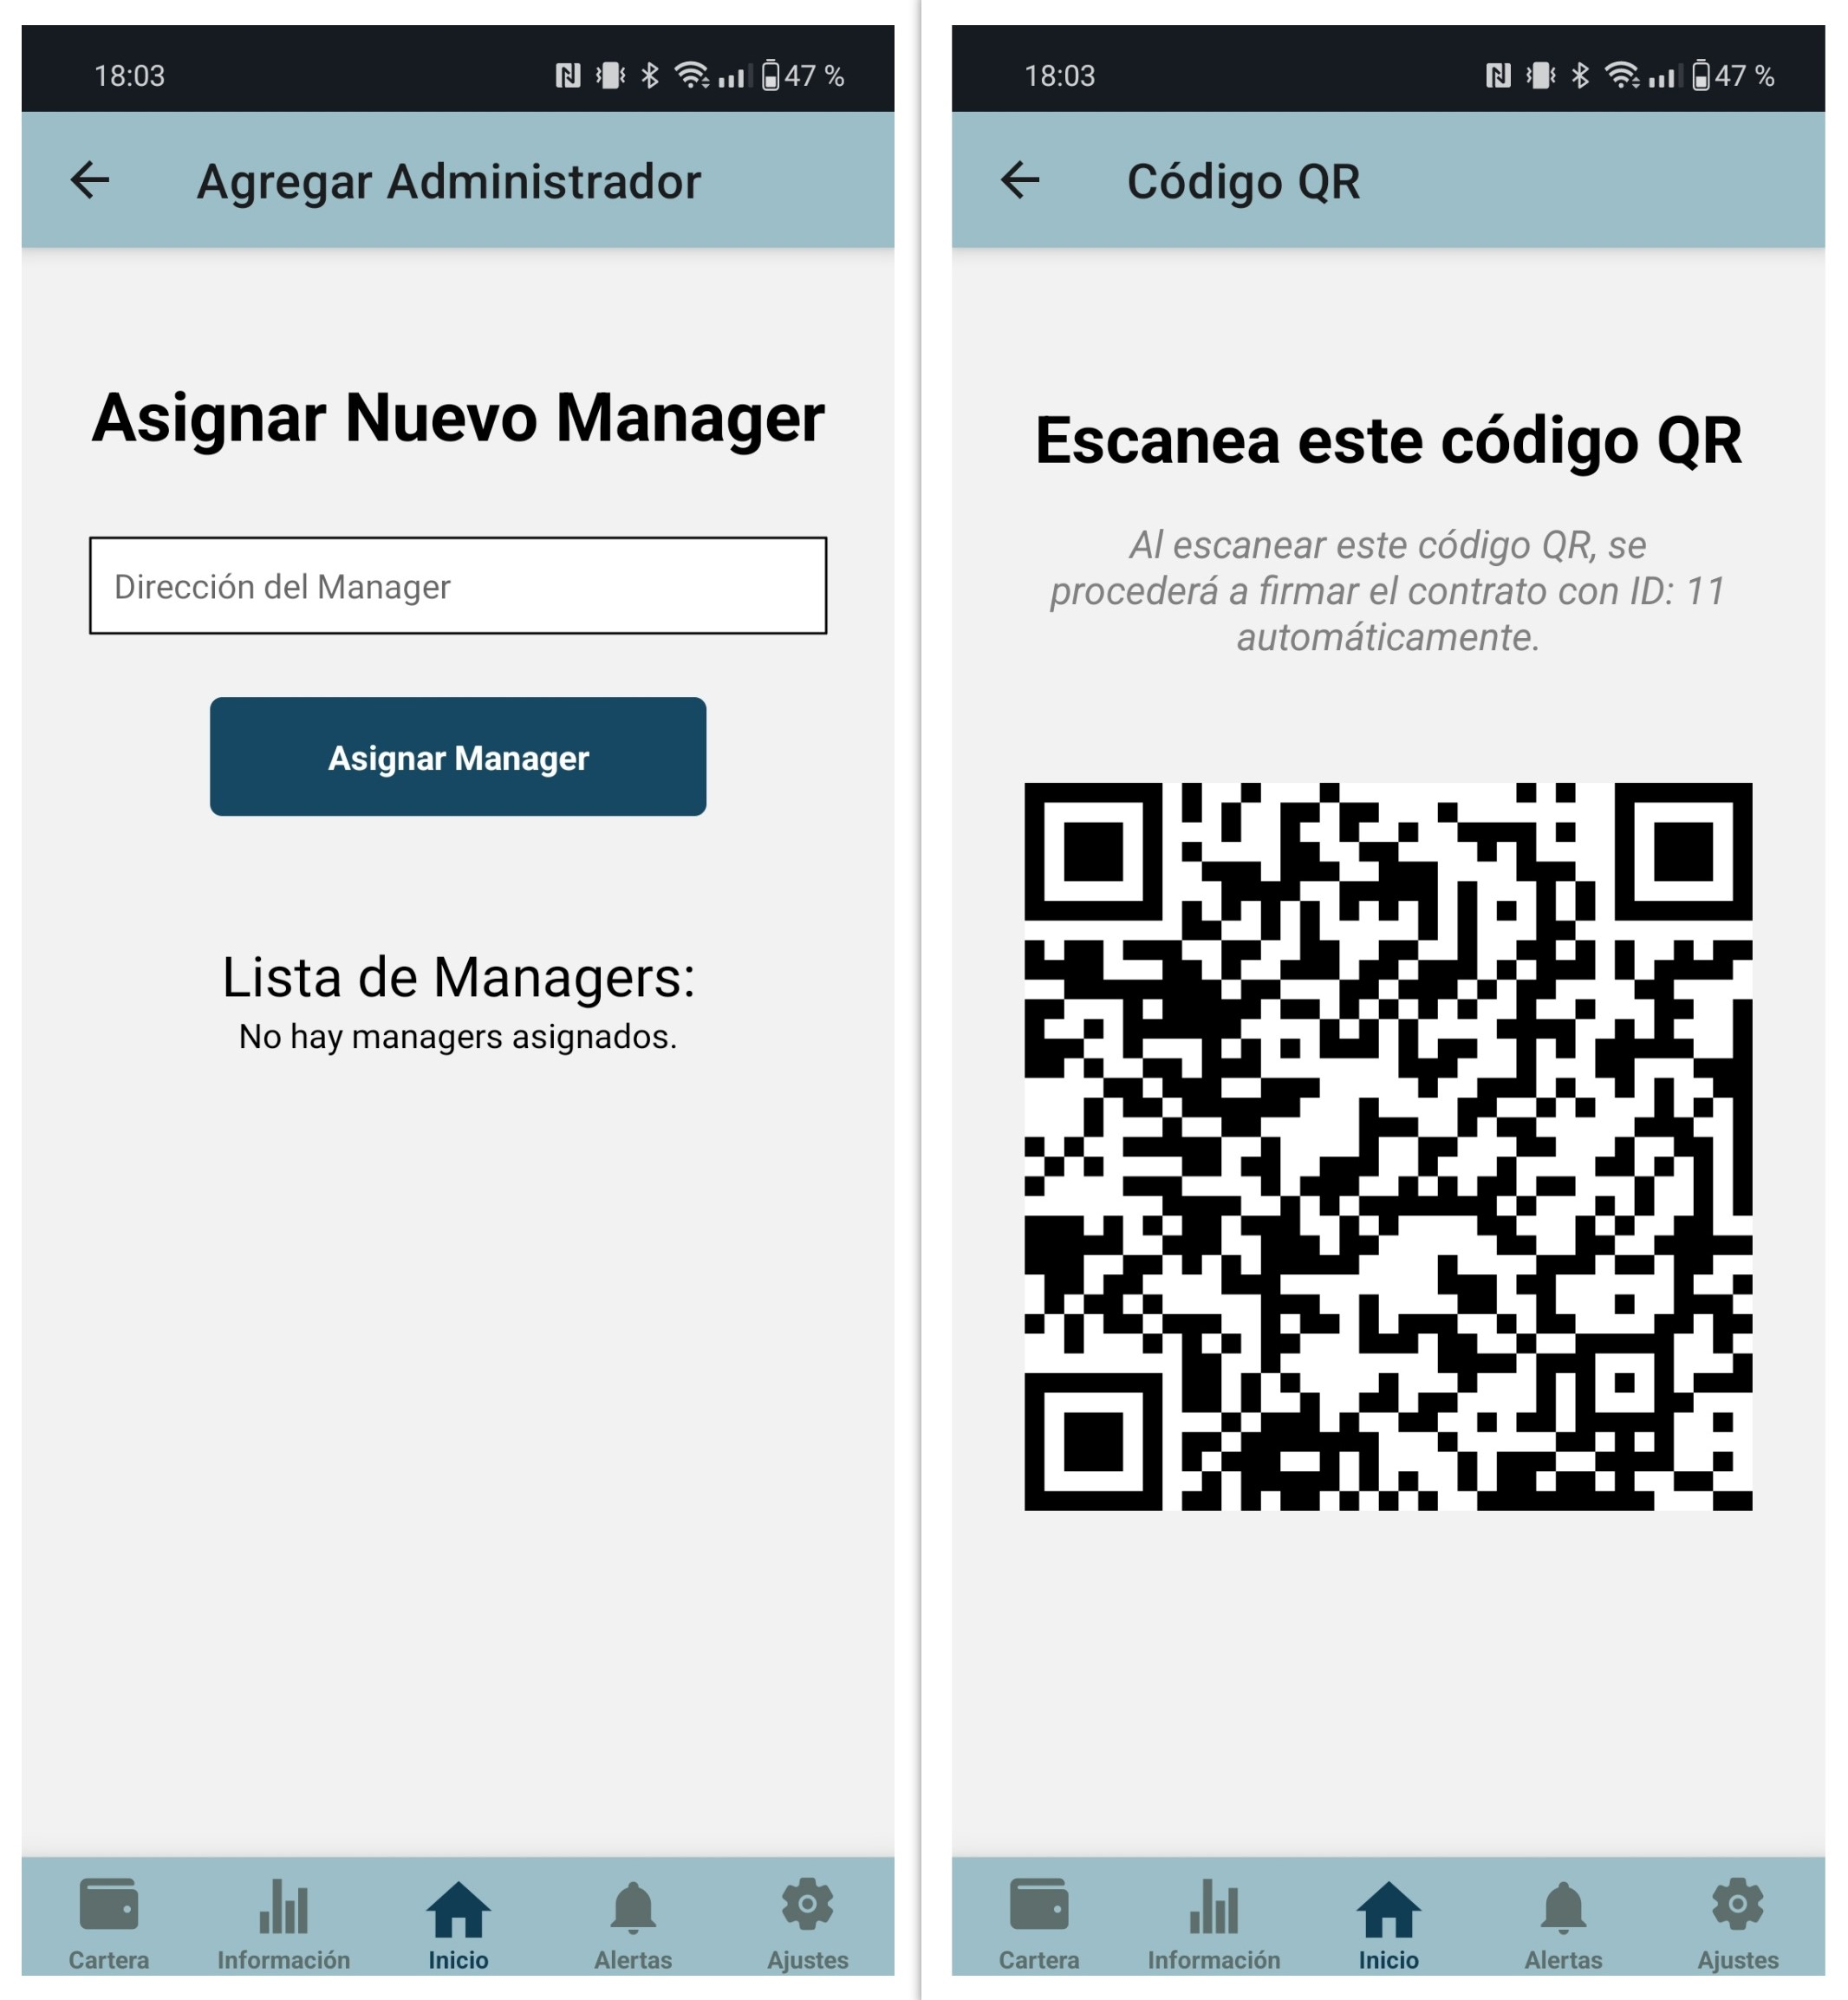
\includegraphics[width=0.90\textwidth]{managerQR}
	\caption[Pantalla añadir mánager y código QR]{Pantallas de gestión de acceso y código QR de un contrato.}
	\label{fig:managerQR}
\end{figure}


\subsection{Alertas}

La pantalla \ref{fig:alertas}, sirve como centro de notificaciones para el usuario, mostrando todos los eventos relacionados con sus contratos.
Cada alerta muestra el ID del contrato al que pertenece, lo que permite una rápida identificación y seguimiento. Además, al seleccionar cualquiera de las alertas, el usuario puede acceder directamente al contrato en cuestión para ver detalles adicionales.

Las alertas que puede recibir un usuario son las siguientes:
\begin{itemize}
\item \textbf{Creación de contrato}: Notifica al usuario cuando es agregado como trabajador a un nuevo contrato.

\item \textbf{Firma de contrato}: informa al empleador cuando el contrato ha sido firmado.

\item \textbf{Liberación de salario}: Avisa cuando el empleador ha liberado el salario correspondiente al contrato.

\item \textbf{Cancelación de contrato}: Alerta cuando un contrato ha sido cancelado por el empleador.

\item \textbf{Finalización de contrato}: Notifica cuando un contrato ha sido concluido por el empleador.

\item \textbf{Propuesta de modificación}: Se informa al usuario cuando el empleador sugiere una modificación al contrato.

\item \textbf{Aceptación o rechazo de modificación}: informa al empleador si su propuesta de modificación ha sido aceptada o rechazada.
\end{itemize}

\begin{figure}[h]
	\centering
	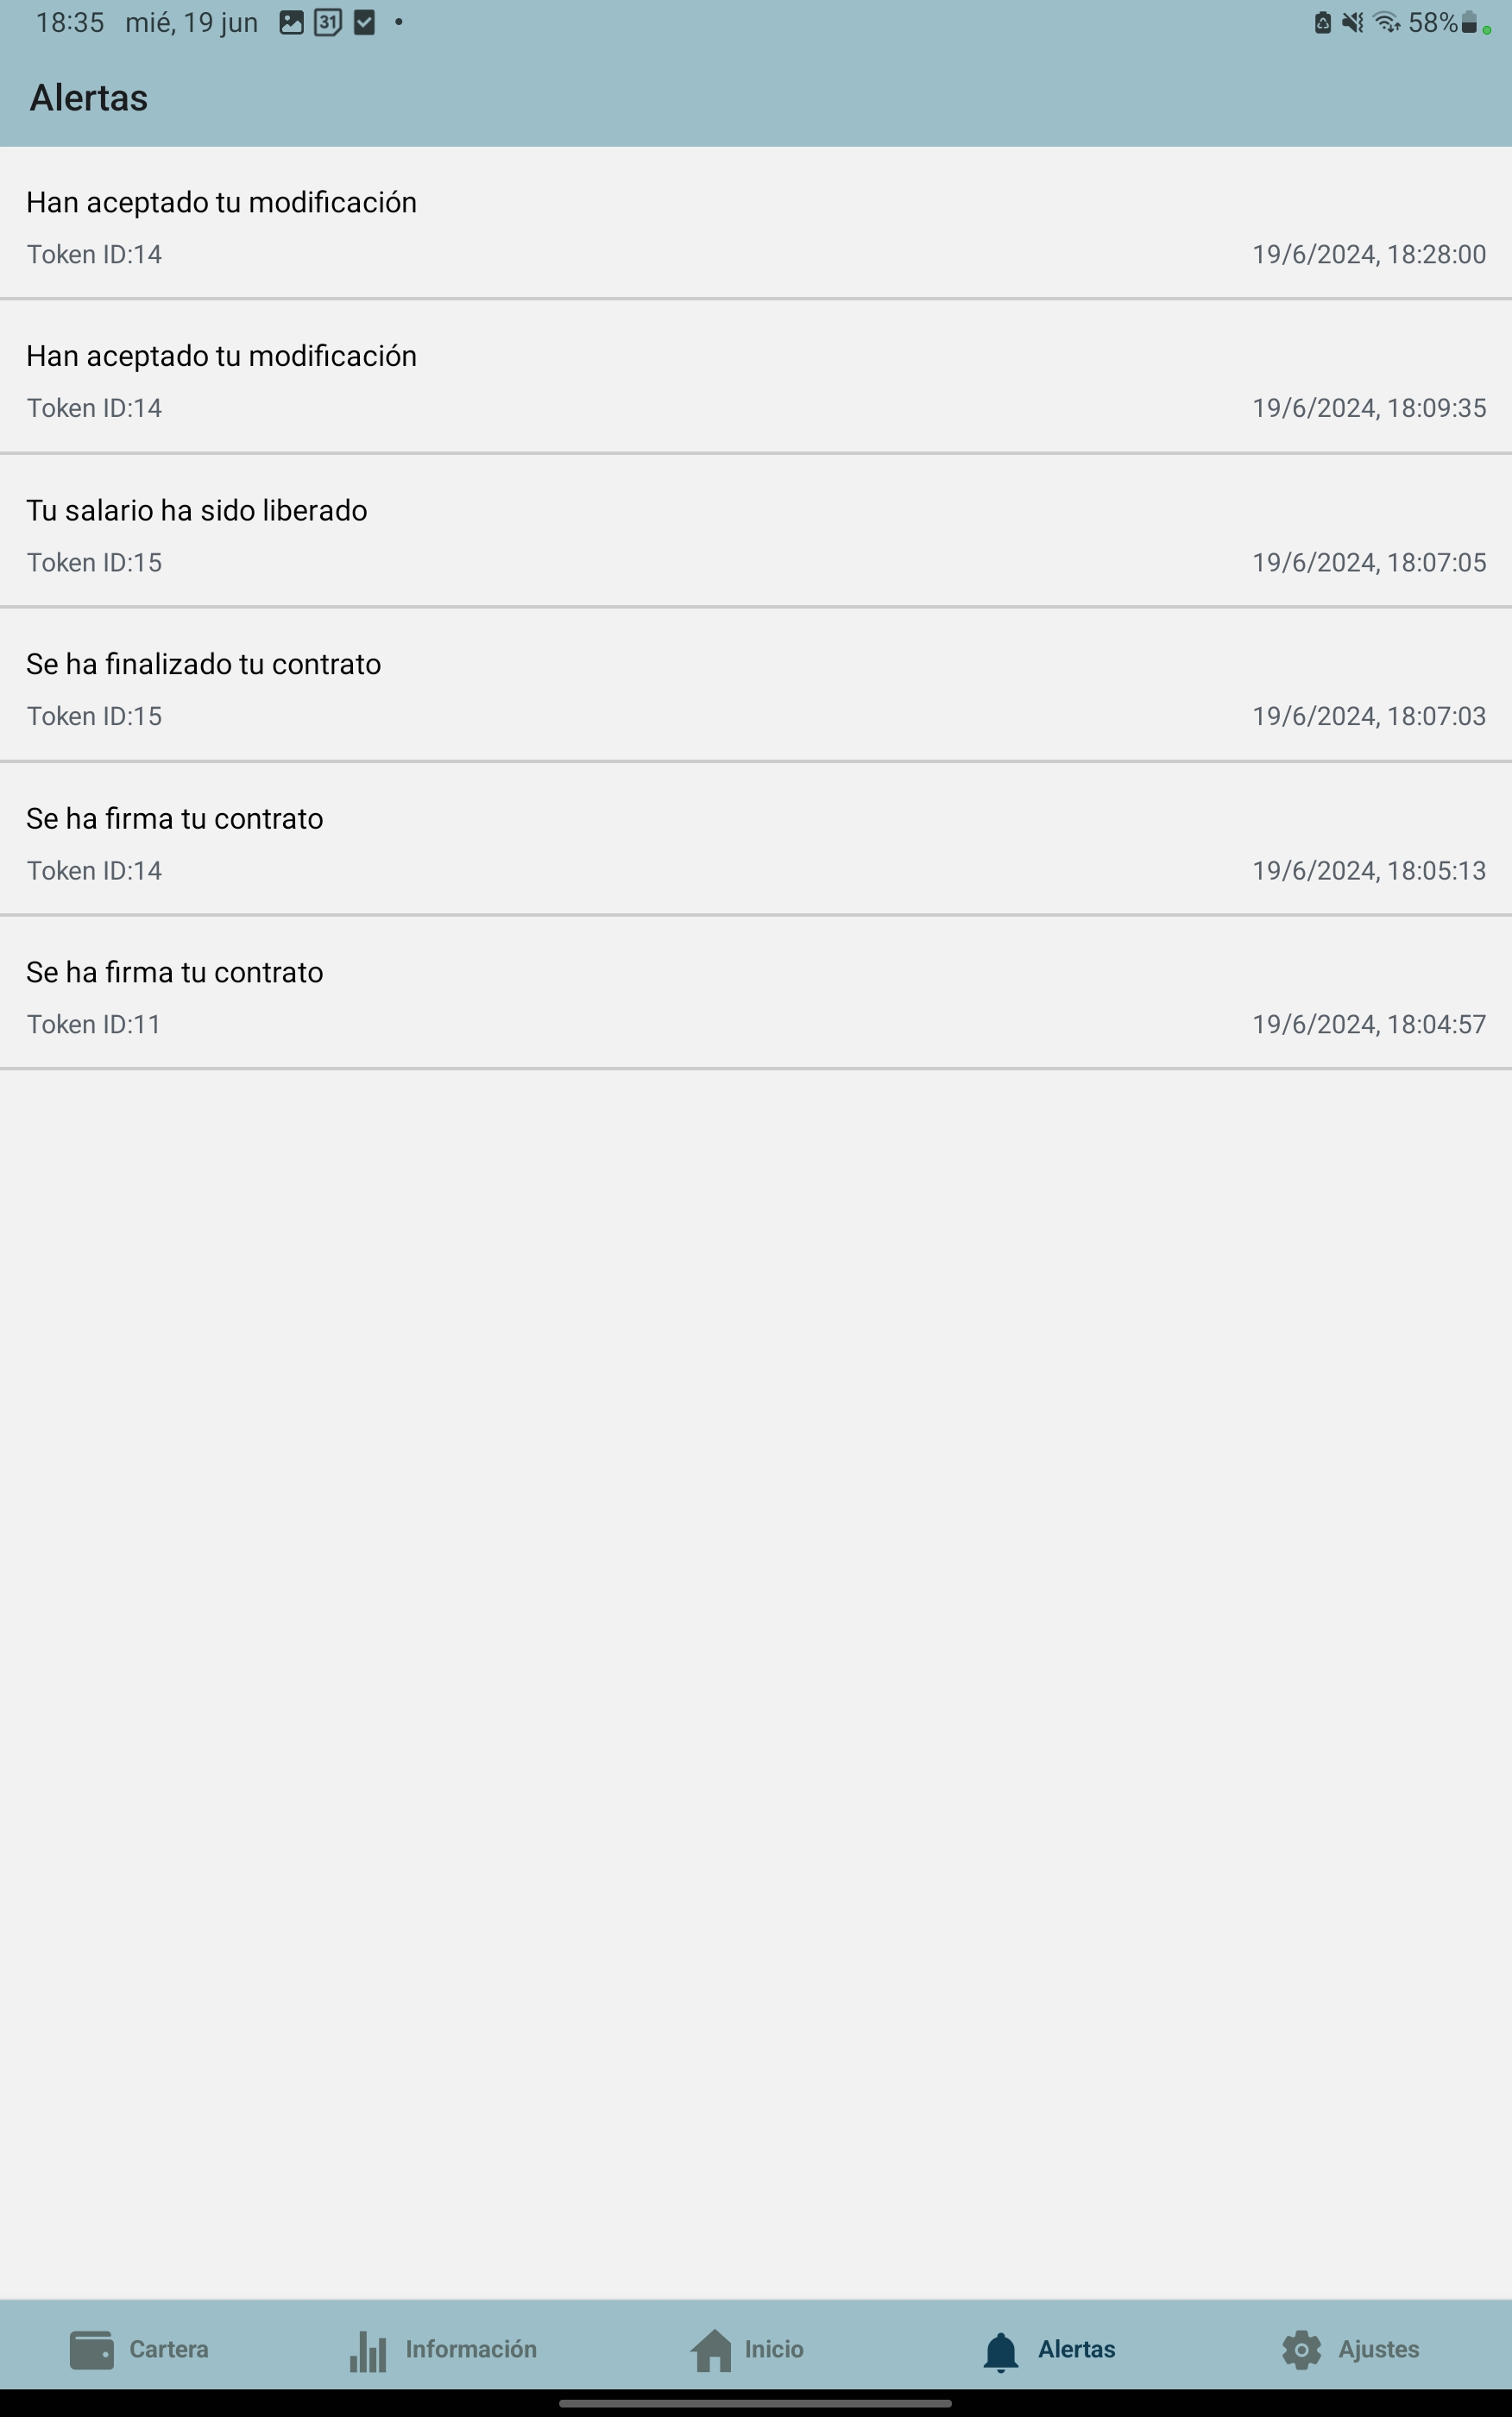
\includegraphics[width=0.50\textwidth]{alertas}
	\caption[Pantalla alertas]{Pantalla de notificación de alertas.}
	\label{fig:alertas}
\end{figure}



\subsection{Cartera}

La siguiente pantalla (ver imagen \ref{fig:cartera}) ofrece un seguimiento detallado de las transacciones financieras dentro de la aplicación.
Lo primero que se muestra en esta pantalla es la dirección de la billetera del usuario actual, seguido del saldo actual en Ether (ETH) de la cuenta.
Seguidamente, se registra cada transacción financiera en la que el usuario ha estado involucrado, detallando a qué contrato pertenece cada una, así como la fecha y hora exactas en que se realizó.

Por un lado, las transacciones que representan un gasto se deben principalmente a dos escenarios: primero, cada vez que se crea un nuevo contrato, se efectúa un depósito inicial; segundo, si se incrementa el salario de un trabajador durante una modificación contractual, esto también resulta en una deducción adicional para cubrir dicho aumento.

Por otro lado, los ingresos pueden surgir de varias maneras: los usuarios reciben dinero cuando se libera el salario, ya sea por la finalización por parte del empleador o porque haya expirado. Además, si un contrato se cancela o el salario se reduce, esto también resulta en la devolución de los fondos sobrantes.

\begin{figure}[h]
	\centering
	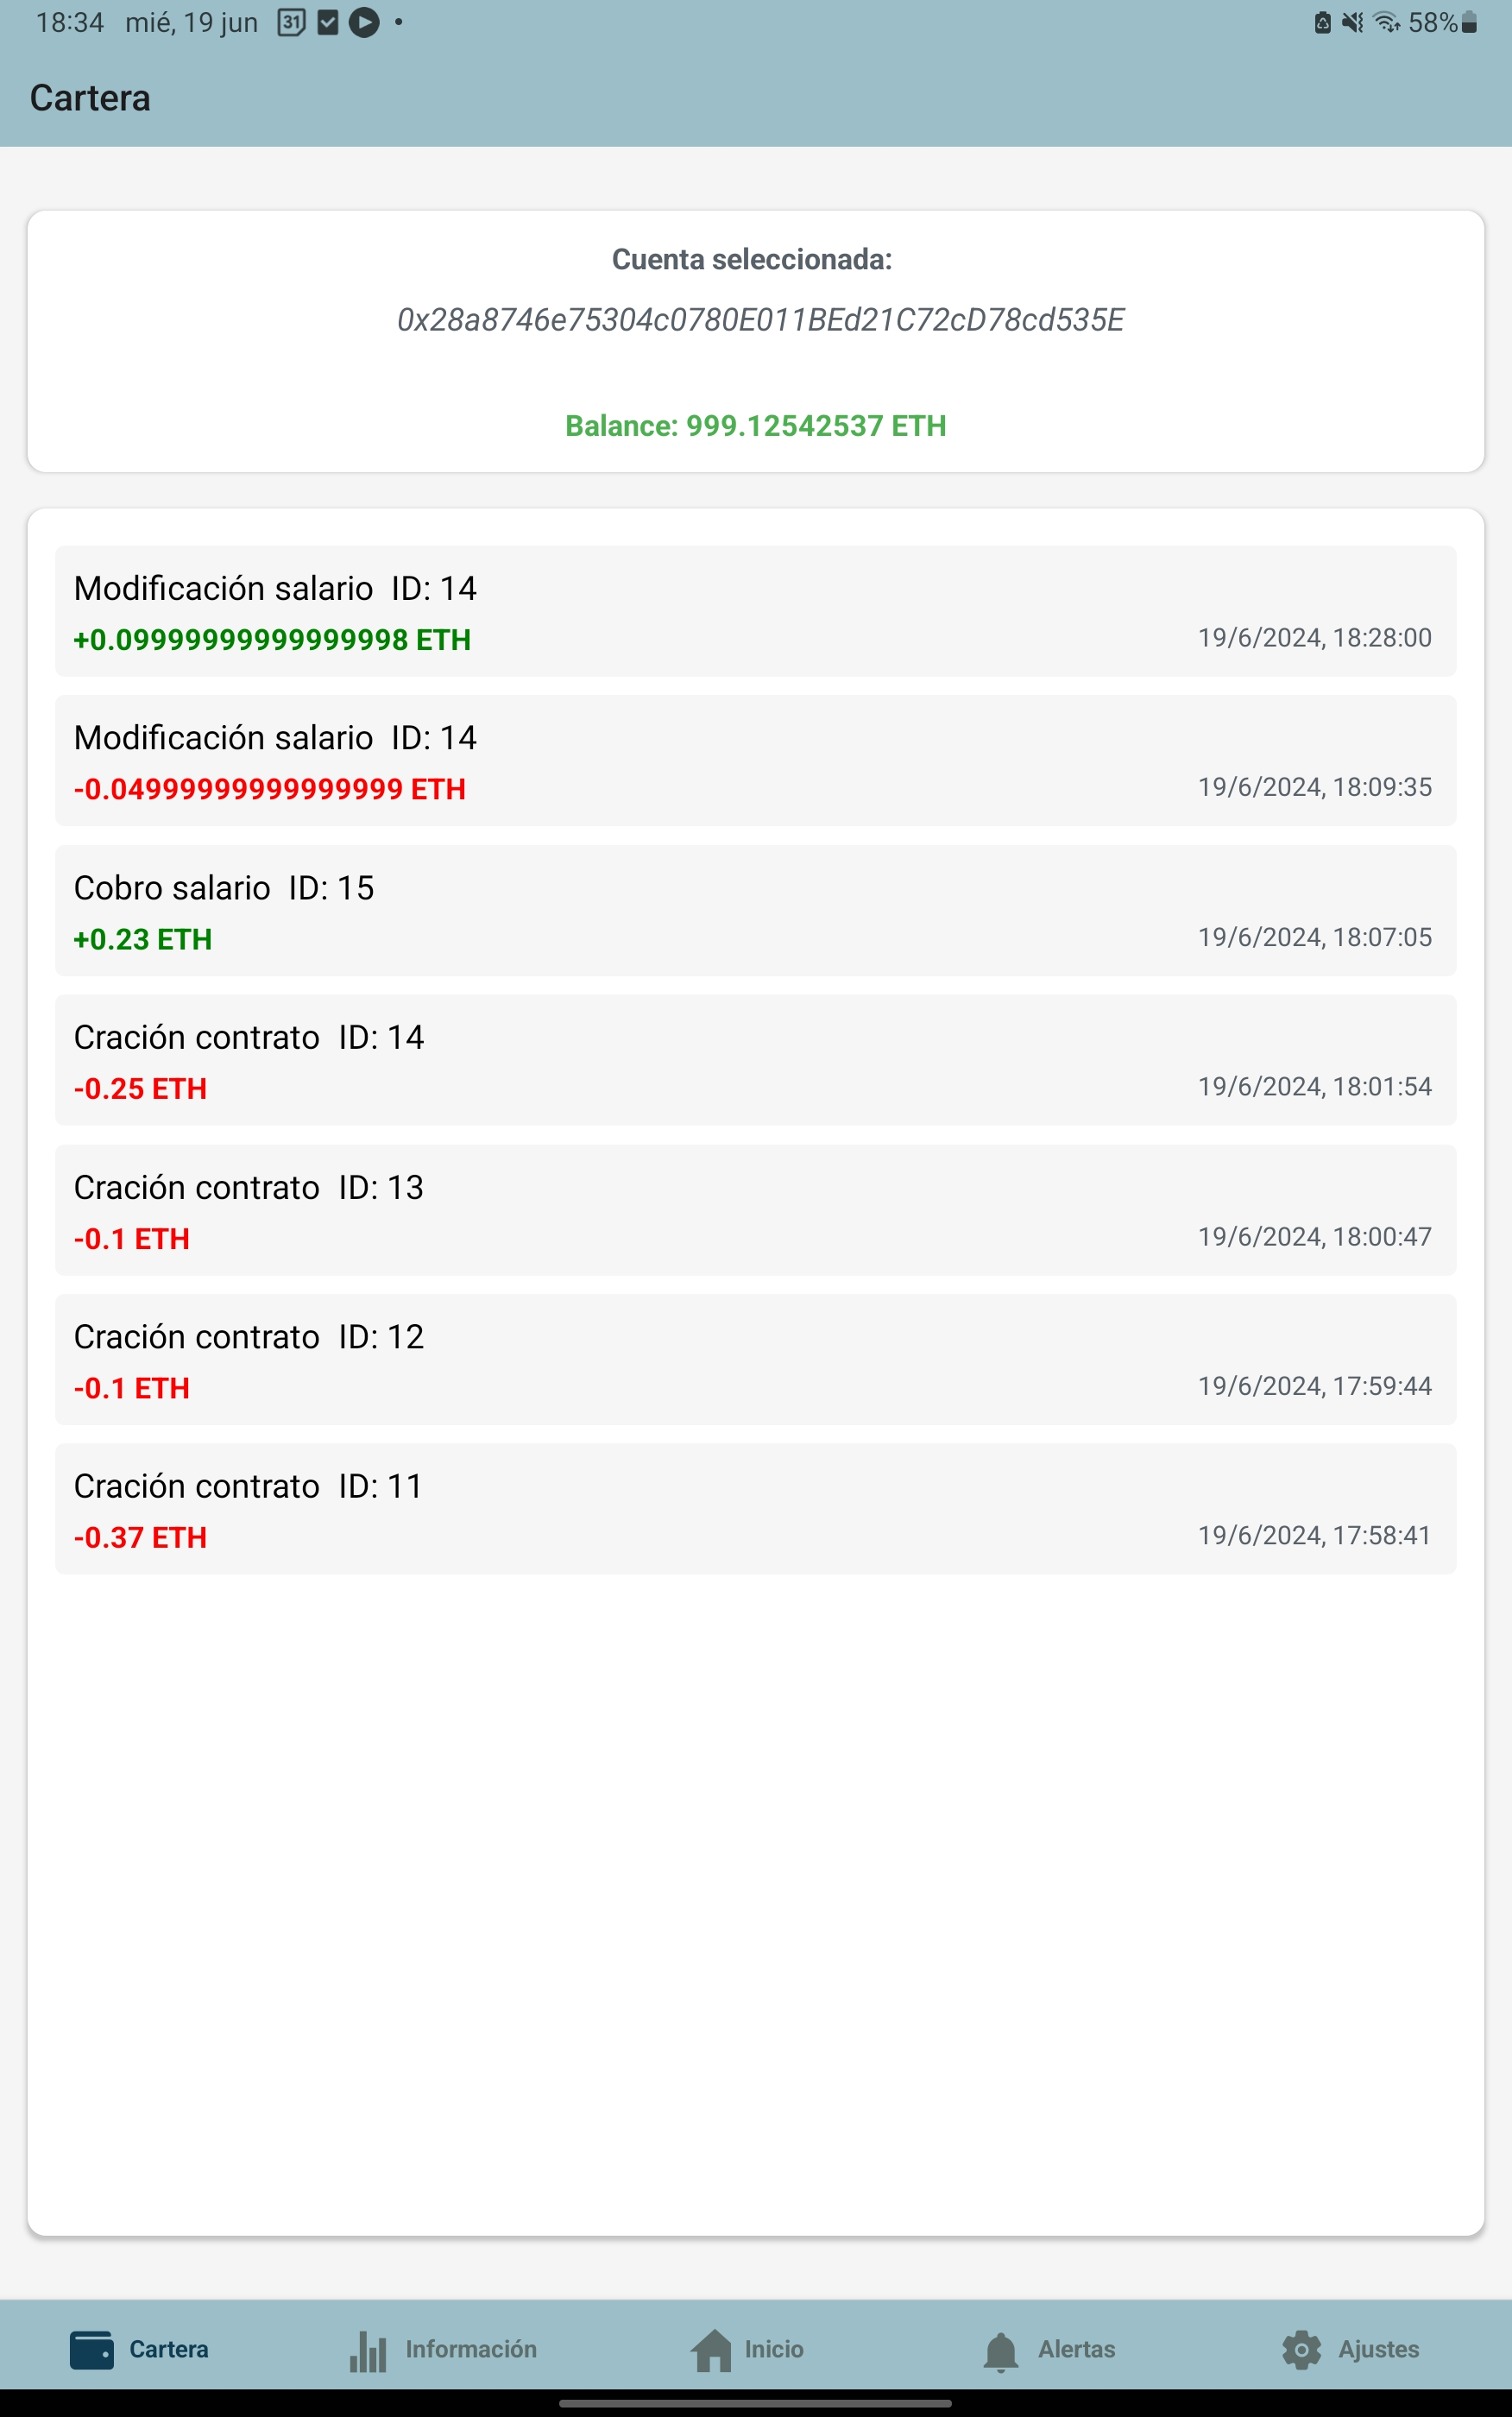
\includegraphics[width=0.50\textwidth]{cartera}
	\caption[Pantalla cartera]{Pantalla que muestra activos y últimos movimientos de la cuenta.}
	\label{fig:cartera}
\end{figure}



\subsection{Pantalla utilidades}

La pantalla \ref{fig:infoHerramientas} está diseñada específicamente para facilitar a los usuarios la gestión y operación con Ethereum.
Esta pantalla proporciona una herramienta que incluye tanto información actualizada sobre el precio del Ethereum en euros como un análisis histórico del mismo a través de un gráfico que rastrea el precio a lo largo del último año.

En la parte inferior de la pantalla, se encuentra un conversor de divisas que permite a los usuarios calcular rápidamente el equivalente de una cantidad dada de euros en Ethereum, y viceversa. Para alternar entre la conversión de euros a Ethereum y de Ethereum a euros, los usuarios simplemente deben pulsar el icono de cambio situado junto a los campos de entrada.
La funcionalidad del conversor es intuitiva, al introducir una cifra en el campo, la conversión se realiza automáticamente, utilizando la tasa de cambio más reciente reflejada en el indicador del precio actual. 

\begin{figure}[h]
	\centering
	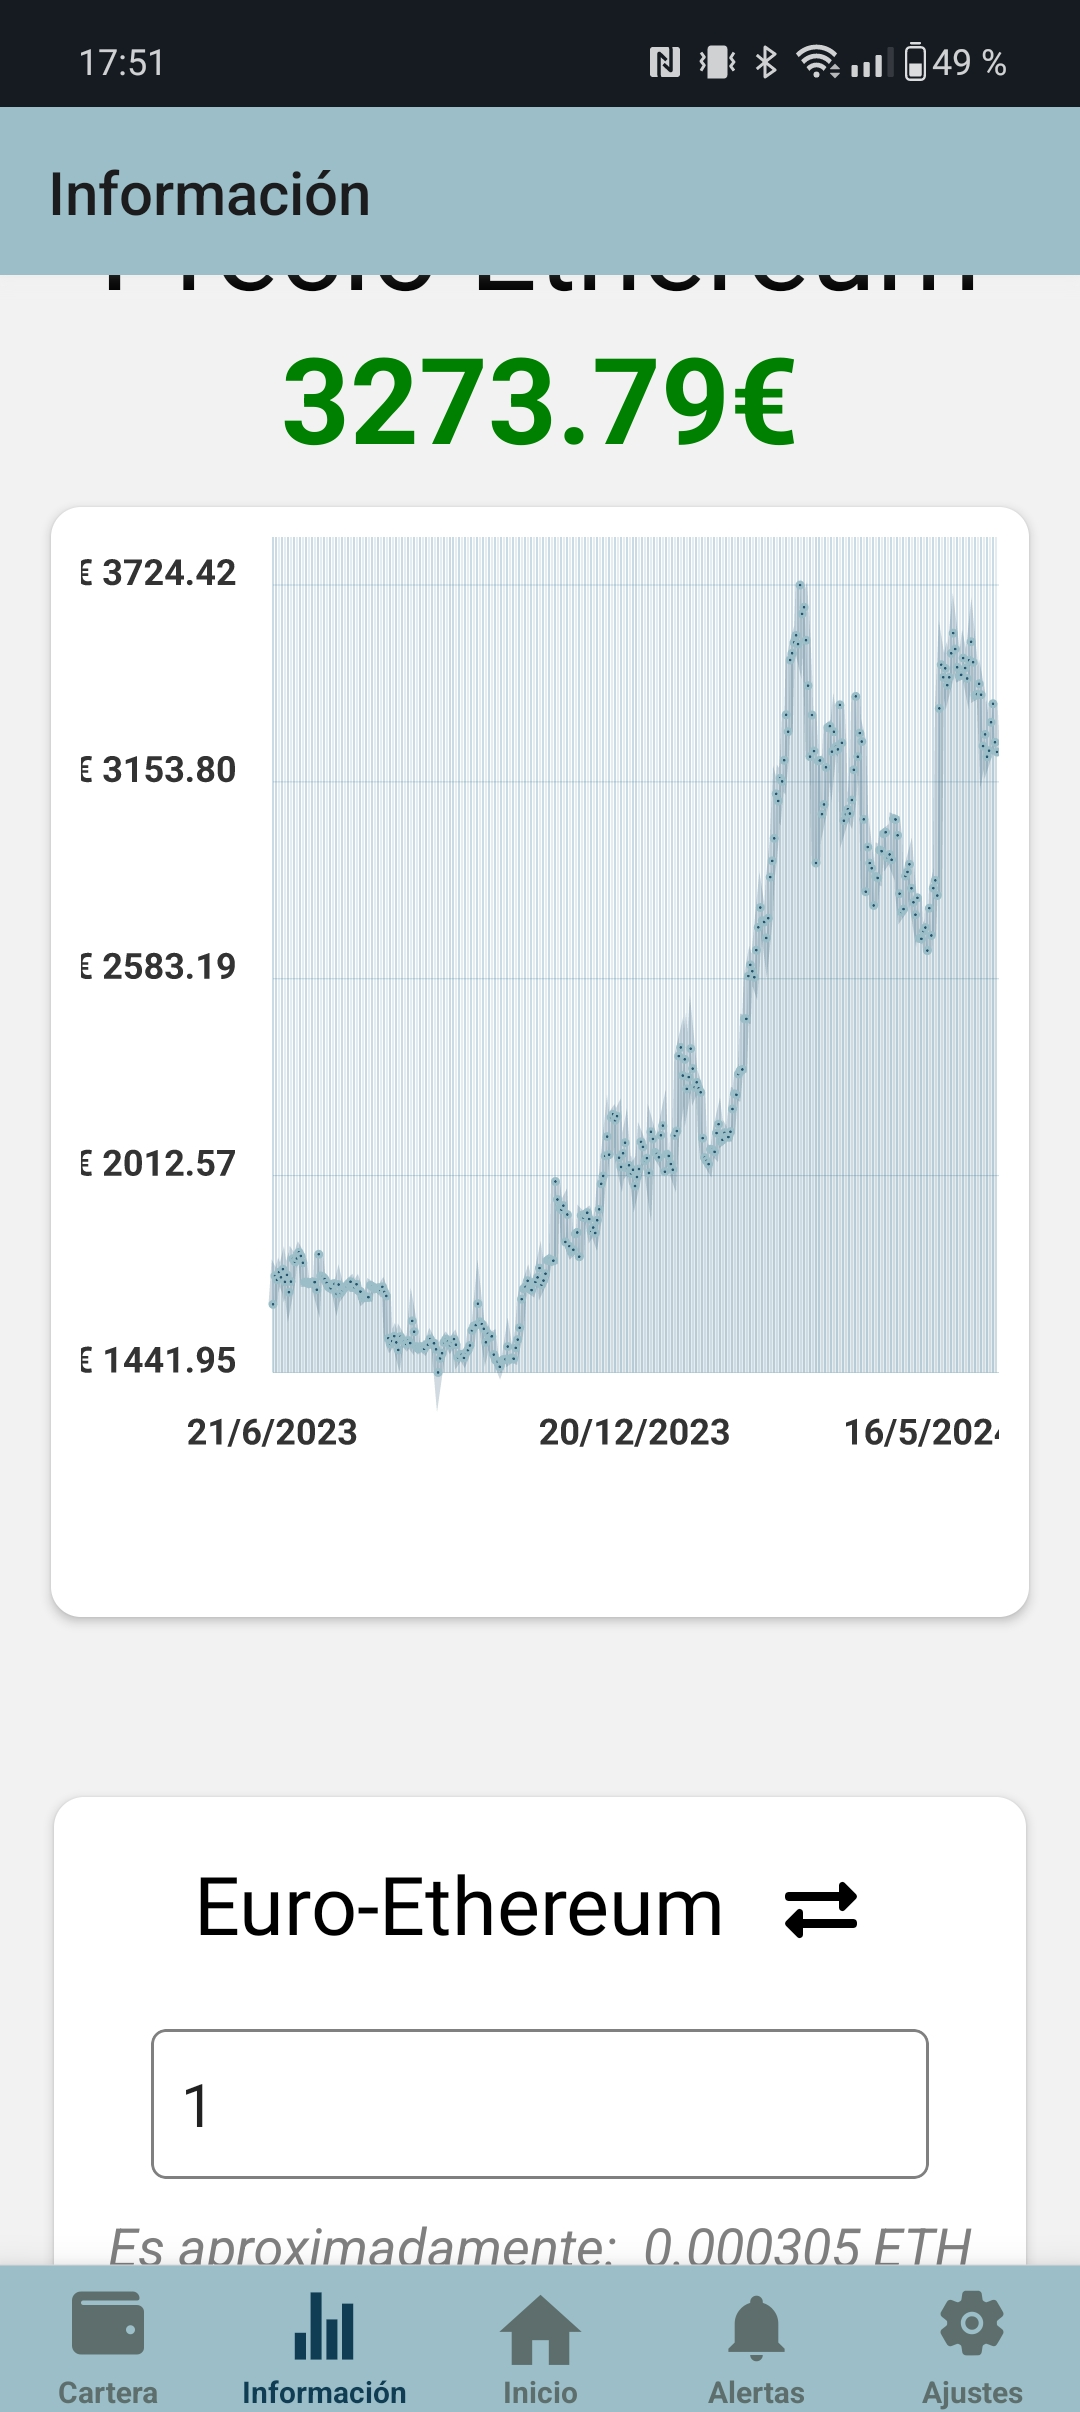
\includegraphics[width=0.40\textwidth]{infoHerramientas}
	\caption[Pantalla utilidades]{Pantallas de información y herramientas.}
	\label{fig:infoHerramientas}
\end{figure}


\subsection{Perfil}

La primera pantalla mostrada en la imagen \ref{fig:perfilModificar}, ofrece al usuario una vista detallada de su perfil, ofreciendo detalles como:

\begin{itemize}
\item \textbf{Nombre}: El nombre completo del usuario.

\item \textbf{Email}: La dirección de correo electrónico asociada con la cuenta.

\item \textbf{DNI}: Número de identificación del usuario.

\item \textbf{Fecha de Nacimiento}: Presentada en el formato día/mes/año.

\item \textbf{Dirección}: Incluye la dirección completa, señalando la calle y ciudad.

\item \textbf{Teléfono}: Número de contacto del usuario.

\item \textbf{Ganache Address}: Dirección de la billetera del usuario.
\end{itemize}

En la parte inferior de la pantalla se encuentra el botón `cerrar sesión', este botón permite al usuario cerrar su sesión activa, garantizando la seguridad de la cuenta. Si el usuario no cierra sesión, su cuenta permanecerá abierta para un acceso rápido en futuras visitas.

Por otro lado, el botón `Modificar perfil' redirige al usuario la pantalla de modificación del perfil (imagen \ref{fig:perfilModificar}).
Esta pantalla ofrece al usuario la posibilidad de mantener su perfil actualizado, pudiendo mediante un desplegable el país y la ciudad, su dirección o su teléfono.
El proceso de actualización concluye con el botón `Guardar perfil' que al ser presionado, guarda todos los cambios efectuados, asegurando que la información del perfil se mantenga actualizada.


\begin{figure}[h]
	\centering
	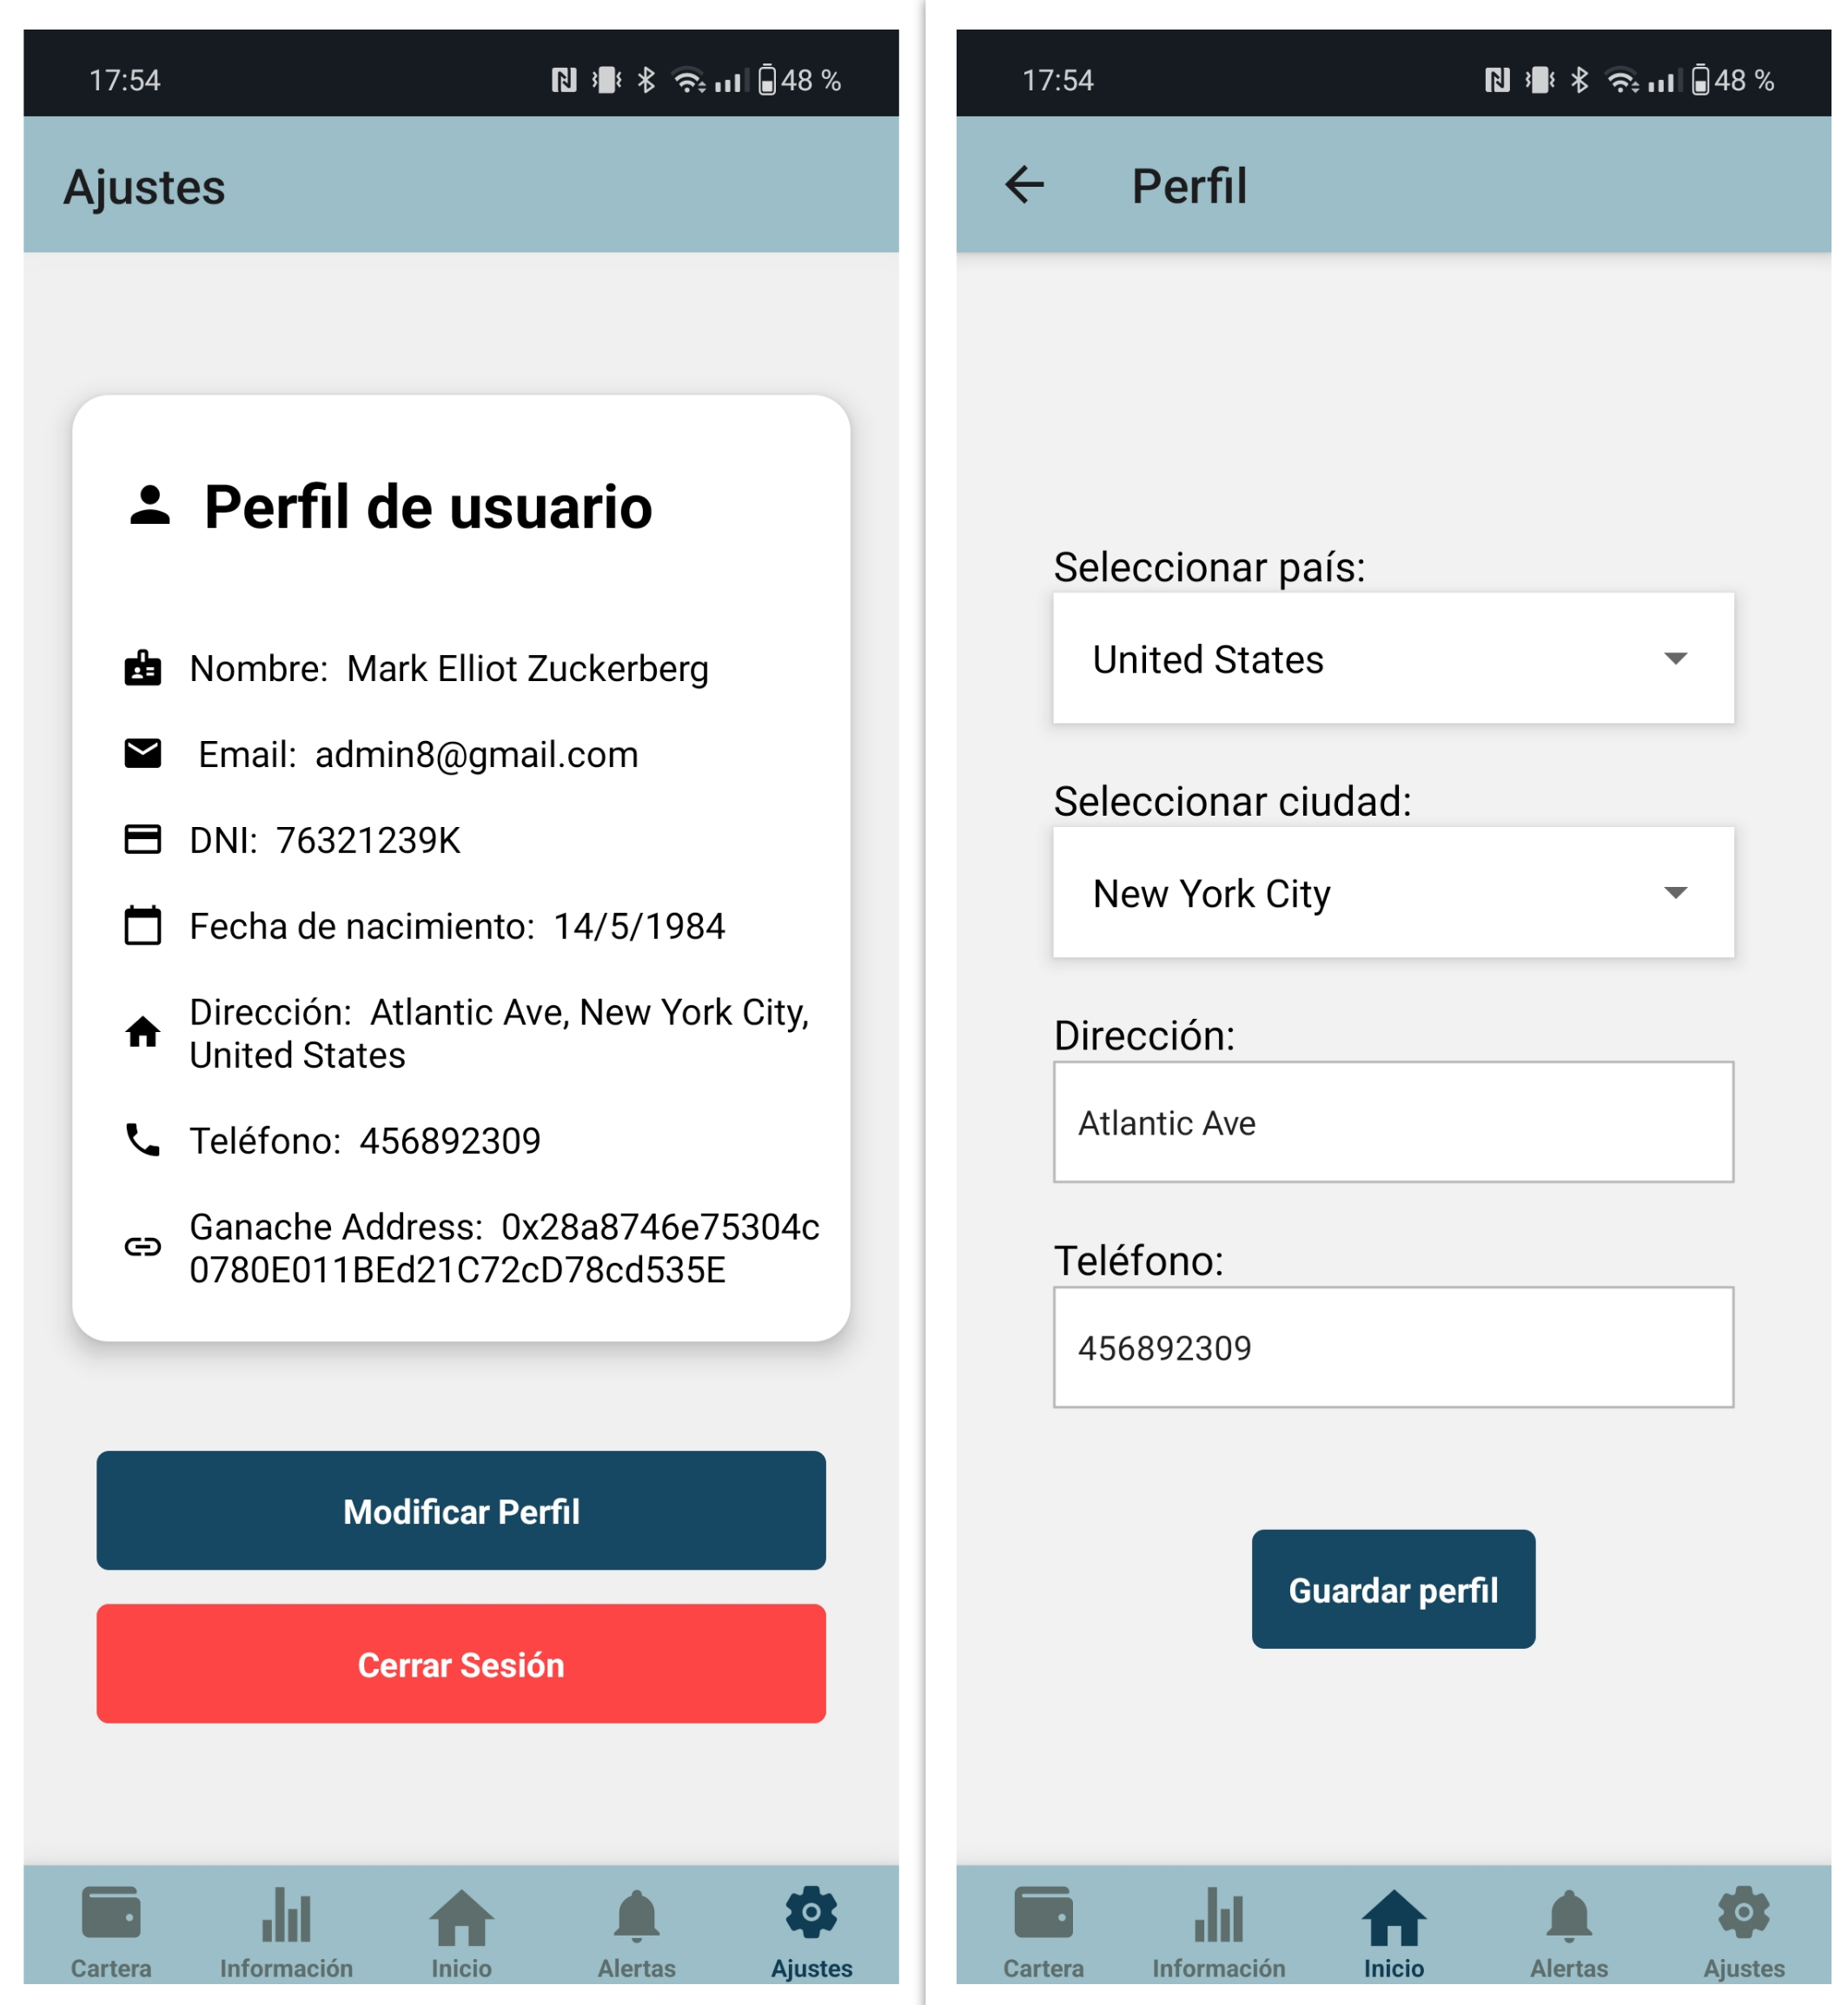
\includegraphics[width=0.90\textwidth]{perfilModificar}
	\caption[Pantallas perfil y modificación perfil]{Pantallas de visualización y modificación de perfil.}
	\label{fig:perfilModificar}
\end{figure}




\apendice{Anexo de sostenibilización curricular}

\section{Introducción}

La transformación digital está remodelando diversos sectores económicos. Sin embargo, algunos sectores como la agricultura, los servicios domésticos y el trabajo freelance enfrentan desafíos significativos en el proceso de contratación y verificación de identidad.
En esta sección, se propone una solución alineada con las directrices de sostenibilidad en el curriculum universitario aprobadas por la CRUE.


\subsection{Sostenibilidad social y económico}

la sostenibilidad social implica la creación de un entorno laboral justo y equitativo.
La utilización de blockchain y contratos inteligentes asegura la transparencia y seguridad en los contratos laborales, garantizando que los términos acordados se cumplan automáticamente y sin intervención manual. 
Este enfoque combate con la informalidad laboral y protege al trabajador, asegurando que se cumplan unas condiciones laborales dignas, en línea con el principio ético de las directrices de sostenibilidad. 

Desde una perspectiva económica, fomentar técnicas legales y justas que aseguren la reducción de la economía sumergida, fortalece la economía formal y aumenta la recaudación fiscal.
Al implementar contratos inteligentes, la aplicación provee un registro inmutable de todas las transacciones, facilitando la fiscalización y el cumplimiento de las normativas.
Esto incrementa la confianza en el sistema laboral y fomenta un desarrollo económico sostenible.


\subsection{Formación para la sostenibilidad}

En el proyecto también se reconoce y se valora la importancia de la educación en sostenibilidad. La formación de los usuarios en el uso de la blockchain y contratos inteligentes refuerza la capacidad de tomar decisiones informadas y responsable, fomentando la cultura de transparencia y equidad en el mercado laboral perseguida con el desarrollo de dicho proyecto.
Esta formación es clave para desarrollar competencias transversales en sostenibilidad.


\subsection{Accesibilidad}

La accesibilidad es crucial en el desarrollo de nuestro proyecto, especialmente enfocado para los trabajadores de sectores marginados, permitiendo el acceso a unas condiciones laborales justas y transparentes.
La aplicación está diseñada para ser simple y accesible desde dispositivos móviles, capaz de ejecutarse en
incluso en dispositivos con muy pocos recursos.
La integración de tecnologías de autenticación biométrica proporciona una capa adicional de seguridad, garantizando la privacidad y protección de la identidad de los trabajadores. 


\subsection{Impacto Medioambiental}

Aunque el foco principal del proyecto se encuentra en la sostenibilidad social y económica, también se considera el impacto medioambiental de la solución. 
La digitalización de procesos laborales reduce la dependencia del papel y disminuye la necesidad de
desplazamientos físicos, contribuyendo a la reducción de la huella de carbono. La eficiencia y automatización proporcionadas por las tecnologías empleadas optimizan el uso de recursos, minimizando el desperdicio y promoviendo prácticas más sostenibles.

\section{Conclusión}

La integración de sostenibilidad en el proyecto presentado aborda de manera integral los desafíos de la economía sumergida y promueve prácticas laborales justas y transparentes. Al adoptar tecnologías disruptivas como blockchain y contratos inteligentes, garantizamos la formalización del empleo, la protección de los derechos de los trabajadores y el desarrollo económico sostenible. 
Este enfoque holístico y transversal busca que no solo mejore la eficiencia operativa sino que también tenga un impacto positivo duradero en la sociedad. Al integrar principios de sostenibilidad en el diseño, promovemos un entorno laboral más justo, seguro y equitativo, alineado con los objetivos de desarrollo sostenible.


\bibliographystyle{plain}
\bibliography{bibliografiaAnexos}

\end{document}
